\documentclass[11pt, a4paper]{article}


\usepackage{wrapfig}
\usepackage{graphicx}
\usepackage[T1]{fontenc}
\usepackage[polish]{babel}
\usepackage[utf8]{inputenc}
\usepackage[font=footnotesize, labelfont=bf]{caption}
\usepackage{csquotes}
\usepackage{placeins}
\usepackage{booktabs}
\usepackage{siunitx}
\usepackage{amsmath}
\usepackage[margin=1in]{geometry}
\usepackage{hyperref}
\usepackage{tabularx}
\hypersetup{
  colorlinks,
  citecolor=black,
  filecolor=black,
  linkcolor=black,
  urlcolor=black
}
\usepackage[backend=biber, sorting=none]{biblatex}
\addbibresource{draft.bib}

\newcommand{\code}[1]{\texttt{#1}}
\linespread{1.3}

\tolerance=1
\emergencystretch=\maxdimen
\hyphenpenalty=10000
\hbadness=10000

\title{Bibliography
management:
\texttt{biblatex}
package}


\author{Krzytsztof
Wiśniewski}
\date{
}


\begin{document}
  \begin{titlepage}
    \centering


    \Large \textbf{UNIWERSYTET GDAŃSKI}\\ \textbf{WYDZIAŁ MATEMATYKI, FIZYKI I
    INFORMATYKI}

    \vspace{2.5cm}


    \large \textbf{Krzysztof Wiśniewski}\\ \textbf{numer albumu: 274276}

    \vspace{1.5cm}
    \raggedright \small Kierunek studiów: Bioinformatyka\\ Specjalność: Ogólna

    \vspace{1.5cm}


    \centering
    \Large \textbf{Optymalizacja oprogramowania do detekcji splątania kwantowego}

    \vfill


    \raggedleft \normalsize Praca licencjacka\\ wykonana\\ pod kierunkiem\\ dr hab. Marcin
    Wieśniak, prof. UG\\

    \vfill


    \centering
    \large Gdańsk 2023
  \end{titlepage}
  \newpage


  \tableofcontents
  \newpage


  \begin{sloppypar}
    \section{Wstęp}
    Closest Separable State Finder (CSSFinder) jest programem pozwalającym na detekcję splątania
    kwantowego układu oraz określenie jak silnie owe splątanie jest. Bazuje on na
    dostosowanym algorytmie Elmera G. Gilberta\cite{Lindemann_Gilbert}, pozwalającym na wyliczenie
    przybliżonej wartości odległości Hilberta-Schmidta (ang. Hilberta-Schmidta distance,
    HSD) pomiędzy stanem a zbiorem stanów separowanych. W literaturze algorytm ten
    pojawia się pod nazwą `kwantowy algorytm Gilberta'(ang. quantum Gilbert algorithm,
    QGA)\cite{MW_Variational_approach}. Działanie tego algorytmu zostało opisane w pracy
    `Hilbert-Schmidt distance and entanglement witnessing' której autorami byli Palash Pandya,
    Omer Sakarya i Marcin Wieśniak\cite{MW_Hilbert_Schmidt_distance}.

    Dr hab. Marcin Wieśniak, prof. UG, utworzył implementację algorytmu QGA w języku Python,
    wykorzystując bibliotekę NumPy do przeprowadzania koniecznych obliczeń macierzowych.
    Wybór ten był podyktowany możliwościami oferowanymi przez taki zestaw narzędzi.
    Pozwalały one w szybki sposób stworzyć prosty kod, zdolny by relatywnie wydajnie przeprowadzać
    obliczenia na wszystkich najpopularniejszych systemach dla komputerów stacjonarnych.

    Zalety języka Python są powszechnie dostrzegane zarówno przez środowiska akademickie,
    jak i komercyjne, co wyraźnie widać w zestawieniach takich jak wydane przez GitHub,
    Inc. `The top programming languages' (2022)\cite{GitHub_Top_languages}. Język Python
    plasuje się w nim na drugim miejscu.

    Alternatywy w postaci języków C, C++ czy Fortran wymagałyby większej ilości bardziej
    skompilowanego kodu, jednocześnie zmuszając do ręcznego skompletowania systemu budowania,
    bibliotek oraz zastosowania dedykowanych rozwiązań dla każdego systemu operacyjnego,
    a przeprowadzanie obliczeń byłoby utrudnione.

    \subsection{Działanie programu}
    Oryginalny program i jego re-implementacja posiadają praktycznie identyczną zasadę działania
    i tylko szczegóły dotyczące sposobu interakcji z nim zmieniły się. Z tego względu w
    dalszej części tekstu sposób działania programu będzie opisywany bez rozgraniczenia
    na wersję oryginalną i re-implementację.

    Program jako dane wejściowe przyjmuje macierz gęstości opisującą pewien stan
    $\rho_{0}$ układu kwantowego. Następnie program w określonych wypadkach jest w stanie
    wydedukować wymiary podukładów i ich liczbę lub można je podać jawnie. Następnie
    dobierany jest stan separowalny $\rho_{1}$. Następnie program postępuje zgodnie z następującymi
    krokami:

    \begin{enumerate}
      \item Zwiększ licznik prób $c_{t}$ o 1. Wylosuj czysty stan produktowy $\rho_{2}$,
        zwany dalej stanem próbnym.

      \item Uruchom preselekcję dla stanu próbnego poprzez sprawdzenie funkcji liniowej.
        Jeśli się nie powiedzie, wróć do punktu 1.

      \item W przypadku udanej preselekcji symetryzujemy $\rho_{1}$ względem wszystkich symetrii
        przez $\rho_{0}$, które respektują separowalność.

      \item Znaleźć minimum $Tr(\rho_{0}- p\rho_{1}- (1 - p)\rho_{2})^{2}$ względem p.

      \item Jeśli minimum występuje dla $0 \le p \le 1$, zaktualizuj
        $\rho_{1}\leftarrow p\rho_{1}- (1 - p)\rho_{2}$, dodać nową wartość $D^{2}(\rho_{0}
        , \rho_{1})$ do listy listy i zwiększyć wartość licznika sukcesu $c_{s}$ o 1.

      \item Przejdź do kroku 1, aż spełnione zostanie wybrane kryterium zatrzymania.
    \end{enumerate}

    Jako dane wyjściowe program zapisuje do plików historię poprawek i stan $\rho_{1}$. Dostępnymi
    kryteriami zatrzymania jest maksymalna ilość korelacji do uzyskania oraz maksymalna ilość
    iteracji do wykonania - ta z tych wartości która zostanie osiągnięta jako pierwsza decyduje
    o zatrzymaniu programu. Jeśli wyznaczona przez program odległość HSD jest
    odpowiednio niewielka (tj. mniejsza niż $1 \cdot 10^{-4}$) stan jest praktycznie separowalny
    w przeciwnym wypadku może być uważany za splątany.

    \subsection{Cele pracy}
    Celami tej pracy sa:

    \begin{itemize}
      \item eksploracja dostępnych metod maksymalizacji wydajności algorytmu QGA,

      \item implementacja algorytmu QGA wybranymi z metod,

      \item weryfikacja poszczególnych z tych rozwiązań pod kątem zmian w czasie pracy programu,

      \item dostosowane postaci i sposób dystrybucji programu do standardów ekosystemu języka
        Python.
    \end{itemize}

    \subsection{Przyczyny przystąpienia do optymalizacji}
    Na ogół rozpatruje się wiele stanów kwantowych, aby zapoznać się z wybranymi obszarami
    przestrzeni stanów kwantowych. Wymaga to więc wielokrotnego wywoływania programu
    CSSFinder na wielu różnych macierzach wejściowych. W naturalny sposób preferowanym jest
    więc aby obliczenia dla jednego stanu trwały jak najkrócej, im mniej czasu zajmą tym
    więcej stanów zostanie zbadanych w tym samym czasie.

    Niestety, język Python wykorzystany do stworzenia oryginalnej implementacji jest powszechnie
    znany z problemów z wydajnością\cite{srinath2017python}. Są one pokłosiem faktu że jest
    to interpretowany język programowania, a więc konieczne jest by specjalny program (tak
    zwany interpreter) wykonywał instrukcje zawarte w kodzie programu. Dodatkowo jest to
    język dynamicznie typowany z bardzo rozbudowanymi możliwościami introspekcji,
    uniemożliwia to zastosowanie wielu z optymalizacji powszechnie wykorzystywanych w
    innych językach programowania. Cechy te są jednocześnie jednymi z największych zalet
    Pythona, obok czytelnej składni i rozbudowanego ekosystemu.

    Aby zwiększyć wydajność, koniecznym jest więc poczynić pewne kompromisy i zrezygnować
    z rozwiązań wygodnych na rzecz rozwiązań bardziej optymalnych dla wydajności.
    Jednocześnie niekorzystnym byłoby od razu sięgać po język asemblera, ponieważ posiada
    on najmniejsze dodatkowe obciążenie i oferuje największą kontrolę nad urządzeniem na
    którym program jest wykonywany. Chociażby ze względu na fakt że program ten będzie:

    \begin{enumerate}
      \item nie przenośny pomiędzy architekturami,

      \item czasochłonny do napisania,

      \item istnieje bardzo niewielka szansa że będzie wydajniejszy,

      \item wielokrotnie bardziej objętościowy.
    \end{enumerate}

    Z tego względu w pracy tej rozważę kilka rozwiązań, czynią mniej radykalne
    kompromisy i wymagając różnej ilości dodatkowego wysiłku aby uzyskać sprawny program.
    Jednocześnie pokażę też, że nie jest konieczne pisanie kodu asemblera własnoręcznie,
    by uzyskać wysoką wydajność.

    \section{Narzędzia}
    \subsection{Kompilacja AOT}
    Kompilacja AOT (Ahead Of Time) to proces tłumaczenia jednej reprezentacji programu (na
    przykład w języku programowania wysokiego poziomu) na inną (na przykład kod
    maszynowy) przed rozpoczęciem pracy kompilowanego programu.

    Obecnie najpowszechniej używana implementacja języka Python, CPython, posiada możliwość
    korzystania z bibliotek współdzielonych (.so - Linux, .dll/.pyd - Windows) które powstały
    w skutek kompilacji kodu wysokiego poziomu. Dostęp do funkcji zawartych w takich
    bibliotekach można uzyskać na kilka sposobów:

    \begin{enumerate}
      \item Przy pomocy API modułu ctypes\cite{Python_ctypes}. Pozwala ono opisać interfejs
        funkcji obcej (tj. takiej która została napisana w języku niższego poziomu i skompilowana
        do kodu maszynowego) i wywołać tak opisaną funkcję.

      \item Poprzez zawarcie w bibliotece odpowiednio nazwanych symboli, automatycznie
        rozpoznawanych przez interpreter języka Python. Takie biblioteki określa się mianem
        modułów rozszerzeń \cite{Extending_Python_With_C_Cpp}. W tym przypadku warto
        dodać, że pomimo, że oficjalna dokumentacja wspomina tylko o językach C i C++, natomiast
        powstały biblioteki które pozwalają wykorzystać w łatwy sposób wiele innych języków
        programowania, takich jak Rust przy pomocy Py03\cite{PyO3} lub GO z użyciem biblioteki
        gopy\cite{gopy}.

      \item Wykorzystując bibliotekę Cython\cite{Cython_Org}\cite{Cython_The_Best_Of_Both}.
        Oferuje ona dedykowany język, o tej samej nazwie, który jest nadzbiorem języka
        Python, który rozszerza jego składnię o możliwość statycznego typowania.
        Biblioteka zawiera transpilator, zdolny przetłumaczyć dedykowany język na C/C++,
        a następnie, wykorzystując osobno zainstalowany kompilator, skompilować do kodu
        maszynowego.

      \item Kompilując kod pythona z użyciem biblioteki mypyc\cite{mypyc}. Ta, podobnie
        do biblioteki Cython, również zawiera transpilator, natomiast zamiast korzystać
        z dedykowanego języka, opiera się on na dodanych w Pythonie 3.5\cite{Python_3_5}
        (PEP 484\cite{PEP_484} i PEP 483\cite{PEP_483}), adnotacjach typów. Jest on
        rozwijany obok projektu mypy - pakietu do statycznej analizy typów dla języka
        Python, również opartej na adnotacjach typów\cite{mypy}.
    \end{enumerate}

    Ponieważ w każdym z wymienionych przypadków, kod niższego poziomu jest kompilowany
    przed dostarczeniem do użytkownika, pozwala to na wykorzystanie zaawansowanych możliwości
    automatycznej optymalizacji dostarczanych przez współczesne kompilatory, na przykład
    LLVM, które jest sercem implementacji clang (język C++) oraz rustc (język Rust).

    \subsection{Kompilacja JIT}
    Kompilacja JIT to proces tłumaczenia jednej reprezentacji programu (na przykład w
    języku programowania wysokiego poziomu) na inną (na przykład kod maszynowy) po rozpoczęciu
    pracy programu. Zazwyczaj wymaga to aby program rozpoczynał pracę w trybie
    interpretowanym, a następne kompilował sam siebie i przechodził w tryb wykonywania skompilowanego
    kodu.

    W momencie pisania tej pracy istnieją dwa szeroko dostępne i aktywnie utrzymywane narzędzia
    oferujące kompilację JIT dla języka Python.

    Pierwszym z nich jest pełna alternatywna implementacja języka Python - PyPy\cite{PyPy_Home_Page}.
    Wykonywana przez nią kompilacja JIT działa on na podobnej zasadzie do uprzednio wymienionych
    - śledzi cały kod który wykonuje i automatycznie decyduje które fragmenty skompilować
    do kodu maszynowego\cite{PyPy_JIT}.

    % ROZWIĄZANIE ODRZUCONE
    % Niestety, posiada ona zasadniczą
    % wadę - jej interfejs binarny\footnote{ang. ABI - Application Binary Interface} oraz
    % programistyczny\footnote{ang. API - Application Programming Interface.} różni się od
    % CPythona, a większość pakietów które normalnie wykorzystują moduły rozszerzeń nie oferuje
    % pre-kompilowanych pakietów dla PyPy. Powoduje to że instalacje takich pakietów są
    % bardzo czasochłonne i obecności kompilatora na urządzeniu docelowym. Dodatkowo, pre-kompilowany
    % kod nie czerpie żadnych korzyści z kompilatora JIT zawartego w PyPy. Problemy te powodują,
    % że PyPy nadaje się głównie do wykonywania aplikacji napisanych w czystym języku
    % Python.

    Drugim narzędziem jest biblioteka Numba\cite{Numba_Article}\cite{Numba_Doc}. Ona, w przeciwieństwie
    do PyPy, wymaga aby fragmenty kodu, które mają być skompilowane, miały postać
    funkcji oznaczonych dedykowanymi dekoratorami.

    % Została ona również zaprojektowana aby dobrze współgrać
    % z biblioteką NumPy. Jej zastosowanie z założenia ma generować wzrost wydajności nawet
    % w sytuacjach gdy kod programu bardzo mocno eksploatuje możliwości biblioteki NumPy.

    % Z uprzednio wymienionych względów dotyczących preferowanych zastosowań powyższych rozwiązań
    % w dalszej części będę próbował wykorzystać bibliotekę Numba, natomiast pominę
    % możliwość skorzystania z PyPy.

    \subsection{Selekcja narzędzi}
    \FloatBarrier
    \begin{table}[ht]
      \centering
      \begin{tabularx}{\textwidth}{c|c|l}
  \hline \textbf{Język programowania} & \textbf{Biblioteki}      & \textbf{Nazwa podprojektu} \\ \hline
   Python                             & NumPy                    & cssfinder\_backend\_numpy \\
   Python                             & NumPy, Cython            & cssfinder\_backend\_numpy \\
   Python                             & NumPy, Numba             & cssfinder\_backend\_numpy \\
   Rust                               & Ndarray                  & cssfinder\_backend\_rust \\
   Rust                               & Ndarray, OpenBLAS        & cssfinder\_backend\_rust \\ \hline
\end{tabularx}
      \caption{Wybrane narzędzia.}
      \label{selected-tool}
    \end{table}
    \FloatBarrier

    Tabela \ref{selected-tool} zawiera zestawienie języków programowania i zastosowanych
    bibliotek użytych do wykonania re-implementacji algorytmu QGA.

    \subsubsection{Python i NumPy}
    Pierwsza wykonana przeze mnie re-implementacja algorytmu, została napisana w języku
    Python, a do realizowania obliczeń na macierzach liczb zespolonych wykorzystywała bibliotekę
    NumPy. Był to dokładnie taki same zestaw, jak wykorzystany do oryginalnej implementacji.
    Podczas przepisywania podjąłem jednak dodatkowe wysiłki aby zastępować kod Pythona
    wywołaniami do funkcji zawartych w bibliotece NumPy. Ponieważ kluczowe dla wydajności
    fragmenty kodu tego pakietu są zaimplementowane w języku niższego poziomu, a
    następnie skompilowane kompilatorem optymalizującym, oferują znacznie wyższą wydajność
    niż analogiczny kod napisany w języku Python. Proces ten pozwolił mi również
    zapoznać się lepiej z charakterystyką programu i udoskonalić interfejs służący do
    komunikacji pomiędzy częścią główną, a samą implementacją (backend'em).

    \subsubsection{Python i NumPy z AOT}
    Następnym wykonanym przeze mnie krokiem było skompilowanie mojej implementacji korzystającej
    z NumPy do kodu maszynowego przy pomocy biblioteki Cython. Kod przeznaczony do
    takiej kompilacji nie musi być adnotowany dedykowanymi informacjami o typach. Zostanie
    on w tedy przetłumaczony na odpowiednie operacje w języku C/C++, a potem
    skompilowany do kodu maszynowego. Brak adnotacji powoduje niestety, że program
    zachowuje swoją dynamiczną naturę, charakterystyczną dla języka Python. Kompilacja
    pozwala jednak usunąć dodatkowy narzut na procesor ze strony interpretera. W takim scenariuszu
    spodziewać należy się, że zyski z kompilacji będą niewielkie, ale mogą wystąpić.

    \subsubsection{Python i NumPy z JIT}
    Ostatnia stworzona przeze mnie re-implementacja w języku Python bazująca na bibliotece
    NumPy dodatkowo korzysta z kompilacji JIT. Pakiet Numba, który został wykorzystany do
    zrealizowania kompilacji JIT, posiada dwa tryby pracy. Pierwszy wykonuje kompilację na
    podstawie specjalnie dostarczonych przez programistę deklaracji typów dla funkcji podlegających
    kompilacji i jest wykonywany zaraz po rozpoczęciu pracy programu\footnote{ang. eager
    (compilation) - niecierpliwa (kompilacja).}. Drugi polega na śledzeniu typów
    wejściowych i wyjściowych funkcji i automatycznie kompiluje funkcję dla tych typów
    danych które są odpowiednio często używane używane\footnote{ang. lazy (compilation)
    - leniwa (kompilacja).}.

    Ponadto, Numba posiada dodatkowe parametry kompilacji, które można przekazać do
    funkcji \code{numba.jit}. Jednym z nich, posiadającym szczególnie duży wpływ na wydajność,
    flaga \code{nopython}. Tryb \code{nopython=True} oferuje znacznie większe możliwości
    optymalizacji i potencjalnie lepszą wydajność. Niestety nie wszystkie funkcje
    dostępne w bibliotece NumPy są akceptowane przez kompilator JIT pakietu Numba w
    trybie \code{nopython=True}. Do niekompatybilnych należy między innymi funkcja
    tensordot która implementuje mnożenie tensorowe. Wspomniana funkcja może zostać skompilowana
    tylko w trybie obiektowym (\code{nopython=False}), który po kompilacji zachowuje dynamiczną
    naturę Pythona. Niestety, brak możliwości skompilowania funkcji używającej tensordot
    powoduje również brak możliwości skompilowania funkcji wyżej w drzewie wywołań. W
    efekcie znacząca część implementacji używającej JIT musi używać trybu obiektowego.

    \subsubsection{Rust i Ndarray}
    Aby uczynić to porównanie jak najpełniejszym, podjąłem również wysiłek zaimplementowania
    części obliczeniowej programu w języku Rust.

    Język ten wybrałem z kilku względów. Przede wszystkim posiada on gotową, rozbudowaną
    infrastrukturę narzędzi pomocniczych. Do tych narzędzi zaliczyć należy menadżera
    pakietów cargo, który zarówno pozwala w łatwy sposób kompilować bardziej rozbudowane
    projekty i tworzyć z nich łatwe do obsługi pakiety, ale również daje możliwość
    korzystania z pakietów udostępnionych przez innych programistów.

    Pozwoliło to w łatwy i szybki sposób skompletować zestaw bibliotek umożliwiających
    wydajne i wygodne tworzenie kodu implementacji algorytmu QGA. Ponadto istnienie biblioteki
    PyO3 znacząco uprościło proces tworzenia interfejsu pozwalającemu interpreterowi języka
    Python na interakcję z tą implementacją.

    Jednocześnie język Rust jest językiem:
    \begin{enumerate}
      \item kompilowanym,

      \item wykorzystującym zestaw narzędzi kompilatora LLVM,

      \item statycznie typowanym,

      \item posiadającym automatyczny system zarządzania pamięcią oparty na koncepcji posiadania
        (ang. ownership), który usuwa konieczność manualnego zarządzania pamięcią,
        zarazem bez konieczności wprowadzania mechanizmu liczenia referencji i
        dedykowanego automatycznego `odśmiecacza' (ang. garbage collector).
    \end{enumerate}

    Cechy te pozwalają oczekiwać, że skompilowany kod będzie osiągał wydajność zbliżoną
    do kodu C/C++, skompilowanych przy pomocy kompilatora clang, który również
    wykorzystuje LLVM do optymalizacji kodu.

    Cały proces wstępnej konfiguracji sprowadził się do około godziny, co stanowi wyśmienity
    wynik, a cały proces implementacji zajął niewiele więcej czasu niż implementacja w
    języku Python. Jednocześnie język Rust posiada system typów który jest w stanie pomieścić
    bardzo dużo informacji o zamiarach programisty. W efekcie kompilator ma możliwość
    wychwycić wiele błędów, których nie może zauważyć kompilator języka C++.

    \subsubsection{Rust i Ndarray z OpenBLAS}
    Biblioteka Ndarray, która jest sercem implementacji w języku Rust, posiada przełącznik
    funkcjonalności\footnote{ang. feature switch} który pozwala wykorzystać funkcje
    zawarte w bibliotece OpenBLAS jako implementację mnożenia macierzowego. Powoduje to niestety,
    że kompilacja programu zaczyna wymagać by biblioteka OpenBLAS była zainstalowana i
    dostępna podczas kompilacji, co jest trudne do uzyskania w środowisku które wykorzystuję
    do kompilacji. W efekcie kompilacja dla wszystkich platform które ma wspierać
    CSSFinder (Windows, Linux i MacOS) jest poza moim zasięgiem, natomiast byłem w
    stanie przeprowadzić ją na komputerze który wykorzystuję do testów wydajności, więc została
    ona wzięta pod uwagę w zestawieniu.

    \section{Metody}
    % Wiele bibliotek korzysta z mieszanek wymienionych powyżej metod, w tym cieszące się dużą
    % popularnością NumPy, CuPy, Tensorflow, czy PyTorch. Dwie ostatnie biblioteki koncentrują
    % się w głównej mierze na uczeniu maszynowym i głównie pod tym kontem są optymalizowane.
    % Ich interfejsy są bardzo zbliżone do NumPy i CuPy, ale brakuje w nich niektórych narzędzi,
    % które nie znajdują zastosowania w dziedzinie sztucznej inteligencji. W dalszej części
    % pracy intensywnie wykorzystywana będzie biblioteka NumPy. Niestety, ze względu na ograniczenia
    % czasowe oraz wstępne przewidywania dotyczące wydajności biblioteka CuPy nie wzięta pod
    % uwagę\footnote{CuPy jest odpowiednikiem NumPy który wykorzystuje do obliczeń GPU. Z tego
    % względu radzi sobie wyśmienicie z operacjami na dużych macierzach, natomiast
    % najprawdopodobniej macierze tutaj rozważane są zbyt małe aby uzyskać wzrost
    % wydajności\cite{CPU_VS_GPU}. Jednocześnie pomimo podobieństwa do NumPy, biblioteka ta
    % różni się i posiada problematyczne zależności (CUDA) co czyni adaptację kodu czasochłonną.}.

    \subsection{Modularyzacja}
    Re-implementując program CSSFinder planowałem wypróbować liczne rozwiązania, które wymagały
    zasadniczych zmian w kodzie algorytmu, w tym przepisania go w innym języku
    programowania. Jednocześnie część programu odpowiadająca za interakcję z użytkownikiem
    i ładowanie zasobów miała pozostawać taka sama. Zdecydowałem więc że tworzony przeze
    mnie kod musi być modularny, aby uniknąć duplikacji wspólnych elementów. Tak też
    program został podzielony na dwie części: główną (`core'), z interfejsem
    użytkowników i narzędziami pomocniczymi oraz część implementującą algorytm (`backend').
    Korpus jest w całości napisany w języku Python i wykorzystuje wbudowany w ten język mechanizm
    importowania bibliotek w celu wykrywania i ładowania dostępnych implementacji algorytmu
    (`backendów'). Dane macierzowe w obrębie korpusu przechowywane są jako obiekty
    ndarray z biblioteki NumPy, ze względu na uniwersalność w świecie bibliotek do obliczeń
    tensorowych (wiele bibliotek w innych językach programowania oferuje gotowe
    narzędzia do transformacji obiektów ndarray na reprezentacje charakterystyczne dla
    tych bibliotek).

    Pozwala to na proste podmiany implementacji o dowolnie różnym pochodzeniu, w tym
    implementacje w językach kompilowanych. Uprościło to znacznie proces weryfikacji zmian
    w zachowaniu programu i przyspieszyło proces tworzenia kolejnych implementacji, jako
    że kod interfejsu programistycznego jest mniej pracochłonny niż kod pozwalający na
    interakcję z użytkownikiem. W przyszłości może to również pozwolić na łatwiejszy rozwój
    nowych implementacji oraz dodawanie nowych funkcjonalności do programu, ponieważ
    będą one mogły być implementowane stopniowo w różnych implementacjach.

    \subsection{Dane testowe}
    Podczas pomiarów konsekwentnie wykorzystywałem ten sam zestaw macierzy gęstości, aby
    móc wygodnie porównywać wyniki wydajności poszczególnych implementacji. W dalszej
    części pracy będę wielokrotnie odnosił się do tych macierzy posługując się symbolem
    $\rho$ z liczbą w indeksie dolnym. Liczba ta będzie wskazywać na konkretną z wymienionych
    poniżej macierzy.

    \FloatBarrier
    \begin{figure}[ht]
      \centering
      \setcounter{MaxMatrixCols}{33}
      
\[
\rho_{0}= \left[
\begin{smallmatrix}
    0.25  & 0 & 0.25  & 0 & 0 & 0 & 0 & 0 & 0 & 0 & 0 & 0 & 0 & 0 & 0 & 0 & 0 & 0 & 0 & 0 & 0 & 0 & 0 & 0 & 0.25  & 0 & 0 & 0 & 0 & 0 & 0 & -0.25 \\
    0     & 0 & 0     & 0 & 0 & 0 & 0 & 0 & 0 & 0 & 0 & 0 & 0 & 0 & 0 & 0 & 0 & 0 & 0 & 0 & 0 & 0 & 0 & 0 & 0     & 0 & 0 & 0 & 0 & 0 & 0 & 0     \\
    0.25  & 0 & 0.25  & 0 & 0 & 0 & 0 & 0 & 0 & 0 & 0 & 0 & 0 & 0 & 0 & 0 & 0 & 0 & 0 & 0 & 0 & 0 & 0 & 0 & 0.25  & 0 & 0 & 0 & 0 & 0 & 0 & -0.25 \\
    0     & 0 & 0     & 0 & 0 & 0 & 0 & 0 & 0 & 0 & 0 & 0 & 0 & 0 & 0 & 0 & 0 & 0 & 0 & 0 & 0 & 0 & 0 & 0 & 0     & 0 & 0 & 0 & 0 & 0 & 0 & 0     \\
    0     & 0 & 0     & 0 & 0 & 0 & 0 & 0 & 0 & 0 & 0 & 0 & 0 & 0 & 0 & 0 & 0 & 0 & 0 & 0 & 0 & 0 & 0 & 0 & 0     & 0 & 0 & 0 & 0 & 0 & 0 & 0     \\
    0     & 0 & 0     & 0 & 0 & 0 & 0 & 0 & 0 & 0 & 0 & 0 & 0 & 0 & 0 & 0 & 0 & 0 & 0 & 0 & 0 & 0 & 0 & 0 & 0     & 0 & 0 & 0 & 0 & 0 & 0 & 0     \\
    0     & 0 & 0     & 0 & 0 & 0 & 0 & 0 & 0 & 0 & 0 & 0 & 0 & 0 & 0 & 0 & 0 & 0 & 0 & 0 & 0 & 0 & 0 & 0 & 0     & 0 & 0 & 0 & 0 & 0 & 0 & 0     \\
    0     & 0 & 0     & 0 & 0 & 0 & 0 & 0 & 0 & 0 & 0 & 0 & 0 & 0 & 0 & 0 & 0 & 0 & 0 & 0 & 0 & 0 & 0 & 0 & 0     & 0 & 0 & 0 & 0 & 0 & 0 & 0     \\
    0     & 0 & 0     & 0 & 0 & 0 & 0 & 0 & 0 & 0 & 0 & 0 & 0 & 0 & 0 & 0 & 0 & 0 & 0 & 0 & 0 & 0 & 0 & 0 & 0     & 0 & 0 & 0 & 0 & 0 & 0 & 0     \\
    0     & 0 & 0     & 0 & 0 & 0 & 0 & 0 & 0 & 0 & 0 & 0 & 0 & 0 & 0 & 0 & 0 & 0 & 0 & 0 & 0 & 0 & 0 & 0 & 0     & 0 & 0 & 0 & 0 & 0 & 0 & 0     \\
    0     & 0 & 0     & 0 & 0 & 0 & 0 & 0 & 0 & 0 & 0 & 0 & 0 & 0 & 0 & 0 & 0 & 0 & 0 & 0 & 0 & 0 & 0 & 0 & 0     & 0 & 0 & 0 & 0 & 0 & 0 & 0     \\
    0     & 0 & 0     & 0 & 0 & 0 & 0 & 0 & 0 & 0 & 0 & 0 & 0 & 0 & 0 & 0 & 0 & 0 & 0 & 0 & 0 & 0 & 0 & 0 & 0     & 0 & 0 & 0 & 0 & 0 & 0 & 0     \\
    0     & 0 & 0     & 0 & 0 & 0 & 0 & 0 & 0 & 0 & 0 & 0 & 0 & 0 & 0 & 0 & 0 & 0 & 0 & 0 & 0 & 0 & 0 & 0 & 0     & 0 & 0 & 0 & 0 & 0 & 0 & 0     \\
    0     & 0 & 0     & 0 & 0 & 0 & 0 & 0 & 0 & 0 & 0 & 0 & 0 & 0 & 0 & 0 & 0 & 0 & 0 & 0 & 0 & 0 & 0 & 0 & 0     & 0 & 0 & 0 & 0 & 0 & 0 & 0     \\
    0     & 0 & 0     & 0 & 0 & 0 & 0 & 0 & 0 & 0 & 0 & 0 & 0 & 0 & 0 & 0 & 0 & 0 & 0 & 0 & 0 & 0 & 0 & 0 & 0     & 0 & 0 & 0 & 0 & 0 & 0 & 0     \\
    0     & 0 & 0     & 0 & 0 & 0 & 0 & 0 & 0 & 0 & 0 & 0 & 0 & 0 & 0 & 0 & 0 & 0 & 0 & 0 & 0 & 0 & 0 & 0 & 0     & 0 & 0 & 0 & 0 & 0 & 0 & 0     \\
    0     & 0 & 0     & 0 & 0 & 0 & 0 & 0 & 0 & 0 & 0 & 0 & 0 & 0 & 0 & 0 & 0 & 0 & 0 & 0 & 0 & 0 & 0 & 0 & 0     & 0 & 0 & 0 & 0 & 0 & 0 & 0     \\
    0     & 0 & 0     & 0 & 0 & 0 & 0 & 0 & 0 & 0 & 0 & 0 & 0 & 0 & 0 & 0 & 0 & 0 & 0 & 0 & 0 & 0 & 0 & 0 & 0     & 0 & 0 & 0 & 0 & 0 & 0 & 0     \\
    0     & 0 & 0     & 0 & 0 & 0 & 0 & 0 & 0 & 0 & 0 & 0 & 0 & 0 & 0 & 0 & 0 & 0 & 0 & 0 & 0 & 0 & 0 & 0 & 0     & 0 & 0 & 0 & 0 & 0 & 0 & 0     \\
    0     & 0 & 0     & 0 & 0 & 0 & 0 & 0 & 0 & 0 & 0 & 0 & 0 & 0 & 0 & 0 & 0 & 0 & 0 & 0 & 0 & 0 & 0 & 0 & 0     & 0 & 0 & 0 & 0 & 0 & 0 & 0     \\
    0     & 0 & 0     & 0 & 0 & 0 & 0 & 0 & 0 & 0 & 0 & 0 & 0 & 0 & 0 & 0 & 0 & 0 & 0 & 0 & 0 & 0 & 0 & 0 & 0     & 0 & 0 & 0 & 0 & 0 & 0 & 0     \\
    0     & 0 & 0     & 0 & 0 & 0 & 0 & 0 & 0 & 0 & 0 & 0 & 0 & 0 & 0 & 0 & 0 & 0 & 0 & 0 & 0 & 0 & 0 & 0 & 0     & 0 & 0 & 0 & 0 & 0 & 0 & 0     \\
    0     & 0 & 0     & 0 & 0 & 0 & 0 & 0 & 0 & 0 & 0 & 0 & 0 & 0 & 0 & 0 & 0 & 0 & 0 & 0 & 0 & 0 & 0 & 0 & 0     & 0 & 0 & 0 & 0 & 0 & 0 & 0     \\
    0     & 0 & 0     & 0 & 0 & 0 & 0 & 0 & 0 & 0 & 0 & 0 & 0 & 0 & 0 & 0 & 0 & 0 & 0 & 0 & 0 & 0 & 0 & 0 & 0     & 0 & 0 & 0 & 0 & 0 & 0 & 0     \\
    0.25  & 0 & 0.25  & 0 & 0 & 0 & 0 & 0 & 0 & 0 & 0 & 0 & 0 & 0 & 0 & 0 & 0 & 0 & 0 & 0 & 0 & 0 & 0 & 0 & 0.25  & 0 & 0 & 0 & 0 & 0 & 0 & -0.25 \\
    0     & 0 & 0     & 0 & 0 & 0 & 0 & 0 & 0 & 0 & 0 & 0 & 0 & 0 & 0 & 0 & 0 & 0 & 0 & 0 & 0 & 0 & 0 & 0 & 0     & 0 & 0 & 0 & 0 & 0 & 0 & 0     \\
    0     & 0 & 0     & 0 & 0 & 0 & 0 & 0 & 0 & 0 & 0 & 0 & 0 & 0 & 0 & 0 & 0 & 0 & 0 & 0 & 0 & 0 & 0 & 0 & 0     & 0 & 0 & 0 & 0 & 0 & 0 & 0     \\
    0     & 0 & 0     & 0 & 0 & 0 & 0 & 0 & 0 & 0 & 0 & 0 & 0 & 0 & 0 & 0 & 0 & 0 & 0 & 0 & 0 & 0 & 0 & 0 & 0     & 0 & 0 & 0 & 0 & 0 & 0 & 0     \\
    0     & 0 & 0     & 0 & 0 & 0 & 0 & 0 & 0 & 0 & 0 & 0 & 0 & 0 & 0 & 0 & 0 & 0 & 0 & 0 & 0 & 0 & 0 & 0 & 0     & 0 & 0 & 0 & 0 & 0 & 0 & 0     \\
    0     & 0 & 0     & 0 & 0 & 0 & 0 & 0 & 0 & 0 & 0 & 0 & 0 & 0 & 0 & 0 & 0 & 0 & 0 & 0 & 0 & 0 & 0 & 0 & 0     & 0 & 0 & 0 & 0 & 0 & 0 & 0     \\
    0     & 0 & 0     & 0 & 0 & 0 & 0 & 0 & 0 & 0 & 0 & 0 & 0 & 0 & 0 & 0 & 0 & 0 & 0 & 0 & 0 & 0 & 0 & 0 & 0     & 0 & 0 & 0 & 0 & 0 & 0 & 0     \\
    -0.25 & 0 & -0.25 & 0 & 0 & 0 & 0 & 0 & 0 & 0 & 0 & 0 & 0 & 0 & 0 & 0 & 0 & 0 & 0 & 0 & 0 & 0 & 0 & 0 & -0.25 & 0 & 0 & 0 & 0 & 0 & 0 & 0.25  \\
\end{smallmatrix}
\right]
\]
      \caption{Macierz $\rho_{1}$.}
      \label{rho-1}
    \end{figure}

    \FloatBarrier

    Pierwsza wymieniana macierz opisuje układ 5 kubitów i posiada wymiary $32\times32$.
    Pomimo że nie zawiera ona wartości, podczas analizy zawsze będzie reprezentowana przez
    macierze zawierające liczby zespolone, ponieważ szczególnie kosztowne obliczeniowo
    części algorytmu wymagają aby części urojone były obecne, co znaczy że usuwanie ich w
    wybranych miejscach nie niesie wymiernych zysków wydajnościowych.

    Następnie w zbiorze macierzy wykorzystywanych jako dane wejściowe znajduje się pięć macierzy
    reprezentujących układy od 2 do 6 kubitów, które przyjmują rozmiary od $4\times 4$
    do $64\times64$. Są one wypełnione zerami poza pierwszym i ostatnim elementem w pierwszej
    i ostatniej kolumnie - te przyjmują wartość $0.5$.

    \FloatBarrier
    \begin{figure}[ht]
      \centering
      \setcounter{MaxMatrixCols}{33}
      \[
        \rho_{n}=
        \begin{bmatrix}
          0.5    & 0      & \hdots & 0      & 0.5    \\
          0      & 0      & \hdots & 0      & 0      \\
          \vdots & \vdots &        & \vdots & \vdots \\
          0      & 0      & \hdots & 0      & 0      \\
          0.5    & 0      & \hdots & 0      & 0.5    \\
        \end{bmatrix}_{(2^{n}\times2^{n})}
      \]
      \caption{Ogólna postać macierzy $\rho_{2}- \rho_{6}$.}
      \label{rho-2-6}
    \end{figure}

    \FloatBarrier

    W tekście macierze te będą oznaczane jako $\rho_{2}$ do $\rho_{6}$, w zależności od
    reprezentowanej liczby kubitów\footnote{Tak więc macierz $\rho_{2}$ ma wymiary $4\times
    4$ i reprezentuje 2 kubity, macierz $\rho_{3}$ ma wymiary $8\times8$ i reprezentuje
    3 kubity, macierz $\rho_{4}$ ma wymiary $16\times16$ i reprezentuje 4 kubity, itd. aż
    do $\rho_{6}$, $64\times64$ .}. Macierze te stanowią wygodny zestaw danych do
    weryfikacji ogólnej charakterystyki zachowania alternatywnych implementacji
    algorytmu, pomimo, że wyniki przy ich pomocy uzyskiwane tak bardzo odbiegają od tych
    uzyskiwanych przy pomocy $\rho_{0}$.

    \subsection{Środowisko testowe}
    Podczas pomiarów wydajności wykorzystywałem każdorazowo to samo środowisko testowe. Do
    chłodzenia CPU wykorzystywane było chłodzenie wodne typu AIO, temperatura w pokoju
    oscylowała w okolicy 25°C, procesor podczas testów wydajności nie doświadczał temperatur
    powyżej 80°C.

    \FloatBarrier
    \begin{table}[ht]
      \centering
      \begin{tabular}{llllll}
    \midrule\midrule
    OS              & Ubuntu 22.04.2 LTS 64-bit         \\
    Kernel          & 5.19.0-42-generic                 \\
    Python          & 3.10.6 64-bit                     \\
    NumPy           & 1.23.5                            \\
    Numba           & 0.56.4                            \\
    Cython          & 3.0.0b1                           \\
    GCC             & 11.3.0 64-bit                     \\
    Rust            & 1.68.2 64-bit                     \\\midrule
    CPU             & AMD Ryzen 9 7950X                 \\
    RAM             & 64GB DDR5 5600MHz CL40            \\
    DRIVE           & 512GB SSD GOODRAM CX400 (SATA)    \\\midrule
  \end{tabular}
      \caption{Konfiguracja środowiska testowego.}
      \label{pc-configuration}
    \end{table}
    \FloatBarrier

    \subsection{Profilowanie}
    Podczas prac nad optymalizacją czasu pracy programu kluczowym było stałe zbieranie
    informacji na temat tego które fragmenty kodu pochłaniają najwięcej czasu. Standardowo
    proces zbierania takich danych określa się mianem profilowania i technologie po które
    sięgałem podczas re-implementacji algorytmu posiadają gotowe narzędzia pozwalające na
    skuteczne pozyskiwanie takich danych oraz ich wizualizację.

    Dla kodu w języku Python, implementacja CPython tego języka posiada w bibliotece
    standardowej dwa dedykowane moduły oferujące funkcjonalność profilowania: `profile' i
    `cProfile'. Pierwszy jest zaimplementowany w języku Python, drugi w C. Ponieważ
    drugi z nich posiada mniejszy dodatkowy narzut na procesor, zdecydowałem żeby to na nim
    oprzeć moje analizy. W celu wizualizacji uzyskanych wyników posłużyłem się
    otwartoźródłowym programem Snakeviz\cite{Snakeviz_PyPI}.

    Do zbierania informacji na temat charakterystyki pracy kodu napisanego w języku Rust
    wykorzystałem narzędzie perf pochodzące z pakiety linux-tools-5.19.0-42-generic
    pobranego przy pomocy menadżera pakietów apt-get. Do wizualizacji uzyskanych wyników
    wykorzystałem jedno z otwartoźródłowych narzędzi funkcjonujące pod nazwą hotspot\cite{HOTSPOT}.

    \subsection{Precyzja obliczeń}
    Oryginalny program, jak i pierwsze stworzone przezemnie re-implementacje posługiwały
    się liczbami zespolonymi na bazie liczb zmiennoprzecinkowych podwójnej precyzji.
    Jedna taka liczba zajmuje 64 bity. Jednak w wielu przypadkach taka precyzja obliczeń
    nie jest konieczna do uzyskania poprawnych wyników. Podstawową zaletą wykorzystania
    liczb zmiennoprzecinkowych pojedynczej precyzji, czyli 32 bitowych, jest
    zmniejszenie rozmiaru macierzy. Pozwala na umieszczenie większej części macierzy w pamięci
    podręcznej procesora. Dodatkowo zwiększa to przepustowość obliczeń wykorzystujących
    instrukcje SIMD, ponieważ wykorzystują one rejestry o stałych rozmiarach (128, 256,
    512 bitów) które mogą na ogół pomieścić dwukrotnie więcej liczb 32 bitowych niż 64 bitowych.
    Pozwala to oczekiwać że obliczenia wykorzystujące liczby zmiennoprzecinkowe
    pojedynczej precyzji będą trwały krócej.

    Tworzony przeze mnie kod od początku powstawał z zamysłem umożliwienia wykorzystania
    liczb zmiennoprzecinkowych o różnych precyzjach, dlatego transformacja ta była dość prosta.
    W języku Python, wykorzystując bibliotekę NumPy przejście na liczby pojedynczej precyzji
    wymagało prawie każdorazowego deklarowania że wynik operacji ma posiadać typ complex64
    (cały czas mówimy o liczbach zespolonych które składają się z dwóch wartości
    zmiennoprzecinkowych). Nie wszystkie operacje które przyjmują parametr określający
    typ wejściowy są akceptowane przez kompilator JIT biblioteki Numba gdy jest on
    przekazywany. To ograniczenie można obejść wykonując zmianę typu jako osobną operację
    przy pomocy metody \code{astype()}.

    Warto tutaj zaznaczyć że wszystkie implementacje w języku Python powstają ze
    wspólnego szablony który był ewaluowany przez bibliotekę Jinja2 do różnych wariantów
    kodu, w zależności od tego jakie parametry były do niego przekazywane. Pozwoliło to
    uniknąć wielokrotnego pisania wspólnych fragmentów kodu, a elementy unikalne są dodawane
    warunkowo. Zastosowanie introspekcji do konstruowania odpowiedniego kodu w trakcie
    wykonywania programu mogłoby w znaczący sposób obniżyć wydajność, dlatego zdecydowałem
    się sięgnąć po system bardziej statyczny, który na pewno nie wpływał na czas pracy
    programu.

    W przypadku języka Rust, posiada on dedykowany konstrukt składniowy pozwalający na deklarowanie
    funkcji w oparciu o symbole zastępcze wobec których stawia się zbiór wymagań dotyczących
    wspieranych interfejsów. W efekcie funkcja może zostać wyspecjalizowana żeby
    akceptować zarówno liczby zespolone skonstruowane z liczb zmiennoprzecinkowych
    pojedynczej jak i podwójnej precyzji. Pozwoliło to uniknąć sięgania po zewnętrzne mechanizmy
    do tworzenia szablonów, tak jak było to konieczne w języku Python.

    \subsection{Wykresy}
    Wszystkie wykresy zamieszczone w tej pracy zostały utworzone przy pomocy skryptów w
    języku Python z wykorzystaniem biblioteki matplotlib\cite{Hunter:2007}.

    \section{Wyniki}
    \subsection{Wstępne profilowanie}
    Prace nad optymalizacją kodu rozpocząłem od wstępnego profilowania pracy programu w trybie
    1 (ang. full separability of an n-quDit state) przekazując do obliczeń układ 5
    kubitów opisany macierzą $\rho_{1}$ (Rysunek \ref{rho-1}).

    Program wykonywał proces analizy stanu aż do uzyskania 1000 korekcji. Przekazany limit
    liczby iteracji wynosił 2.000.000 i nie został osiągnięty. Podczas pomiarów, program
    wykorzystywał domyślny globalny generator liczb losowych biblioteki NumPy (PCG64\cite{NumpyDefaultGenerator})
    z ziarnem ustawionym na wartość 0.

    \FloatBarrier
    \begin{figure}[ht]
      \centering
      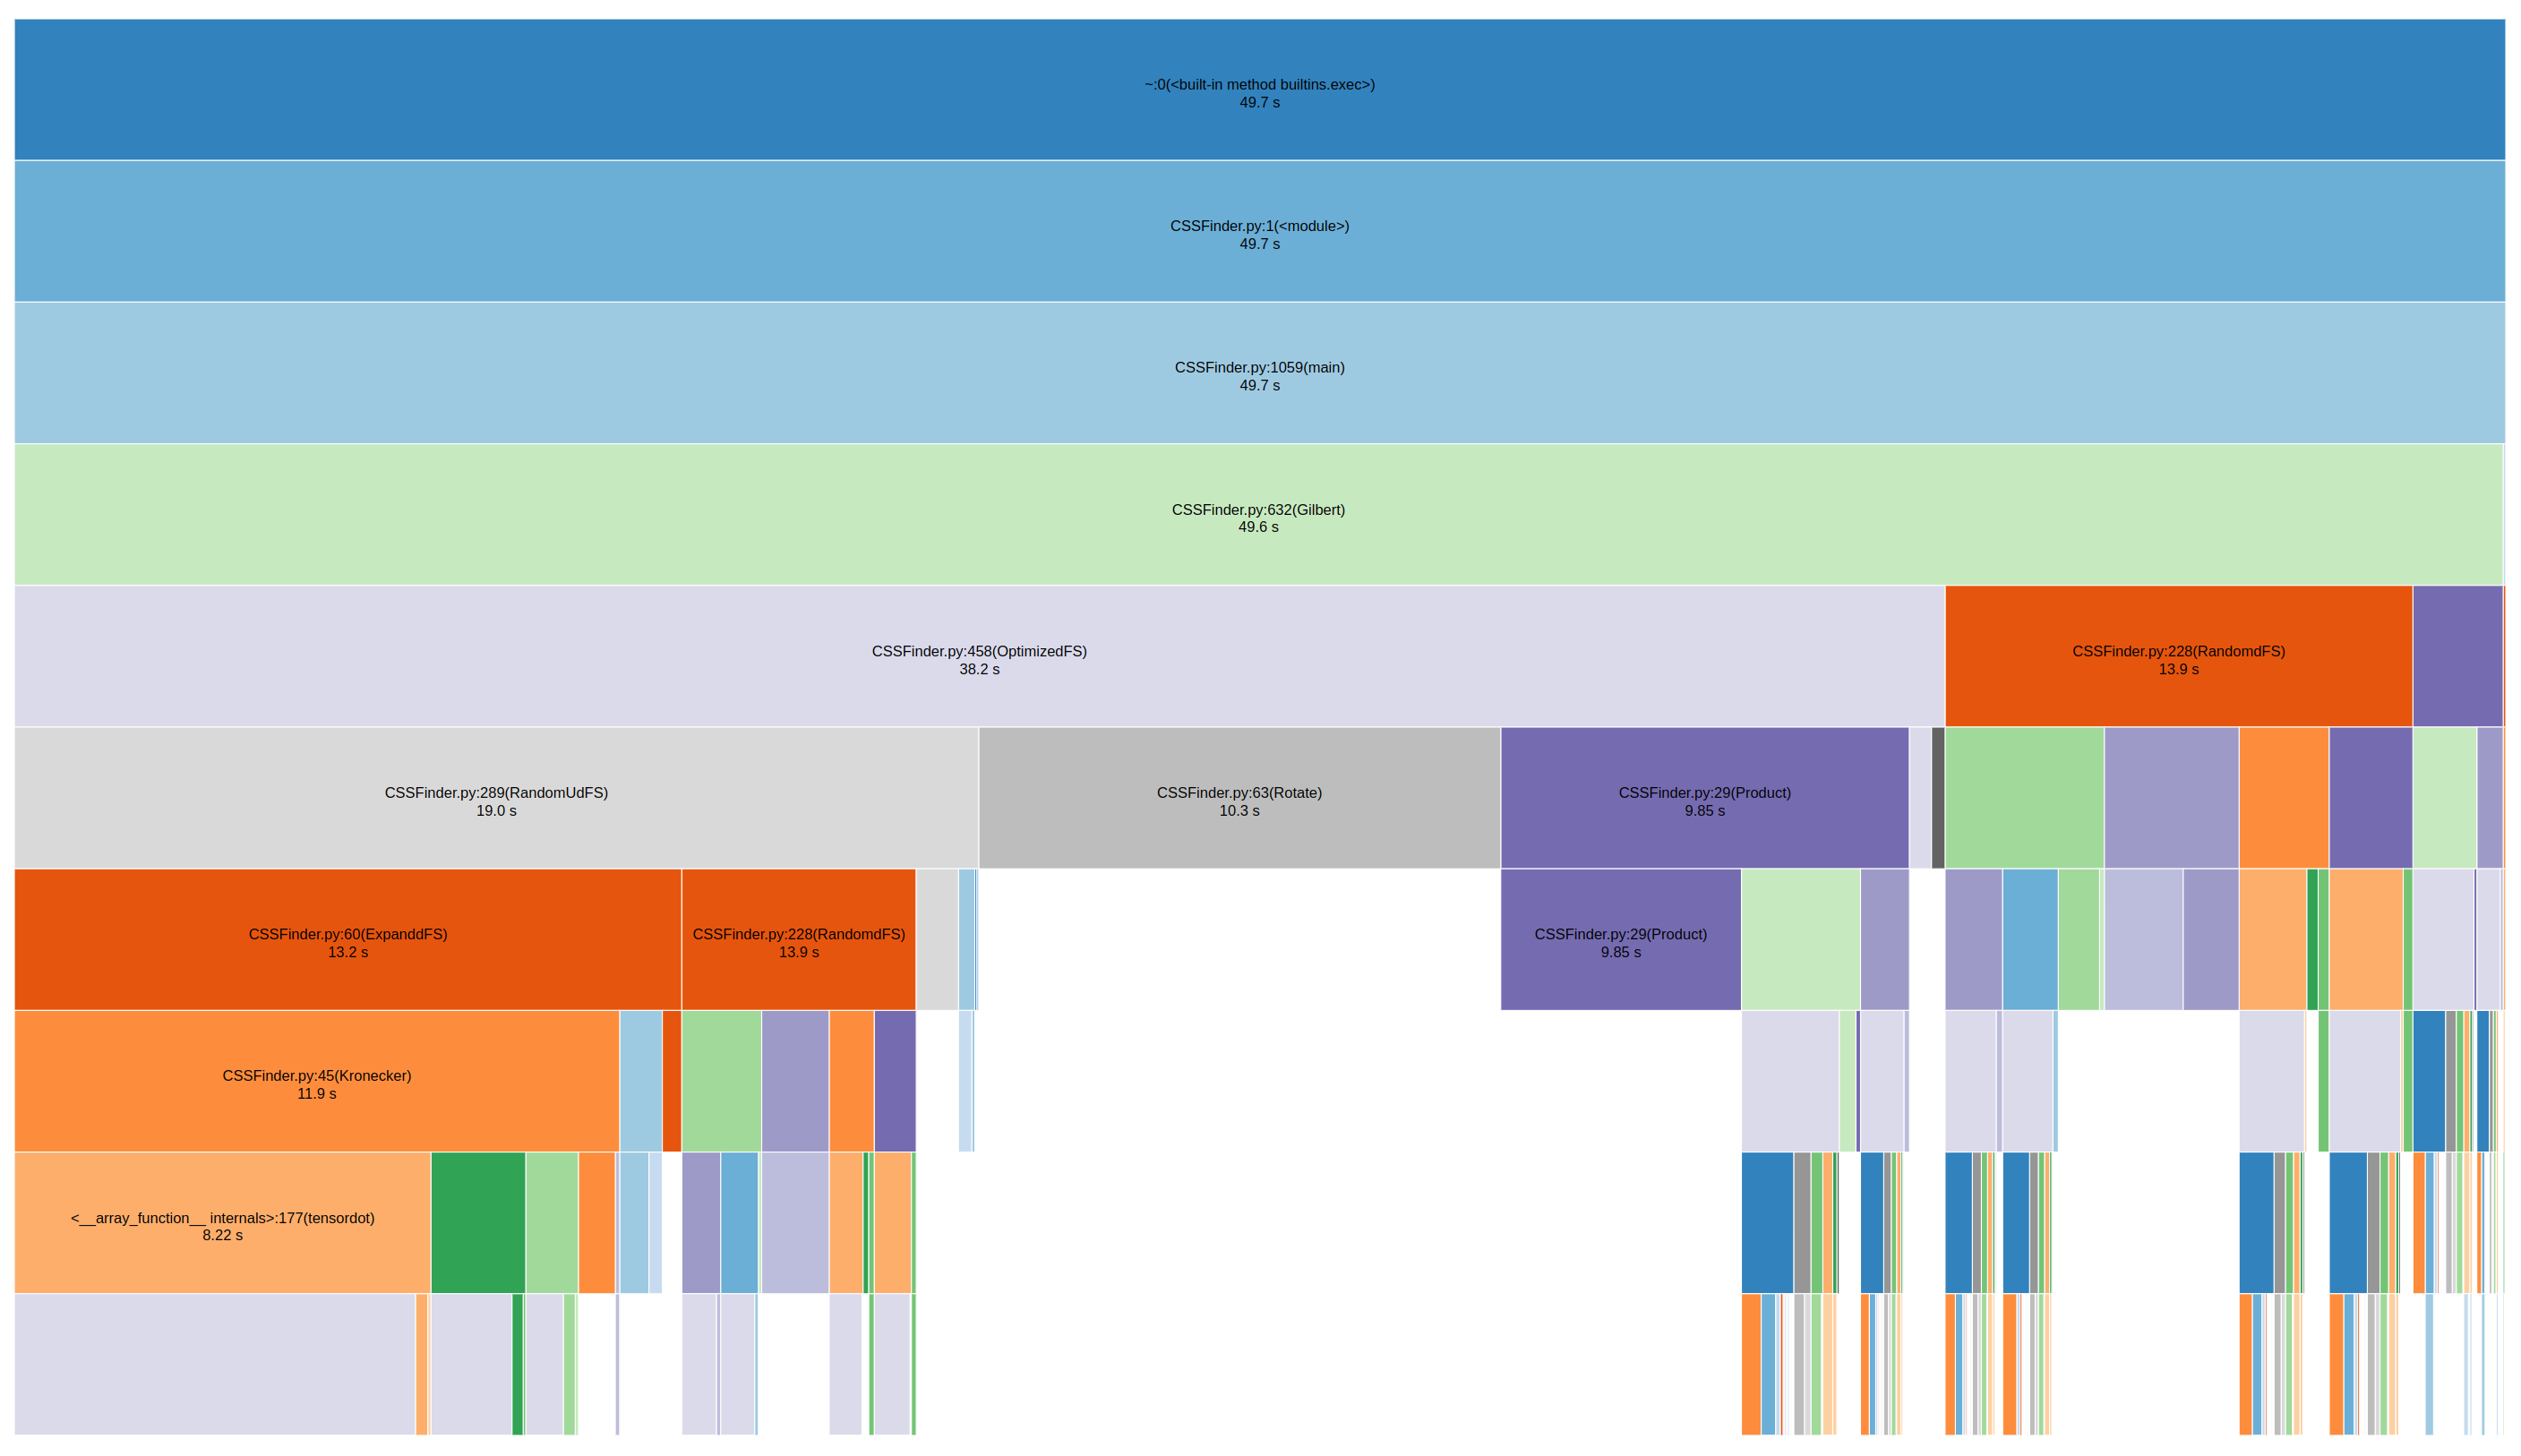
\includegraphics[width=1.0\textwidth]{"resources/profiling_1/graph.png"}
      \caption{Diagram podsumowujący pracę programu wygenerowany przez program Snakeviz.}
      \label{pre-prof-perf}
    \end{figure}
    \FloatBarrier

    Pozwoliło mi to wstępnie przyjrzeć się charakterystyce pracy programu i ocenić czy powszechnie
    dostępne narzędzia mogą zostać wykorzystane w tym wypadku. Rysunek
    \ref{pre-prof-perf} przedstawia diagram, typu Icicle, obrazujący udział czasu, pochłoniętego
    przez wykonywanie poszczególnych funkcji, w całkowitym czasie pracy programu. Pierwszy
    blok od góry (\code{~:0(<built-in method builtins.exec>)}) to wywołanie funkcji
    wykonującej kod programu. Następne bloki, których opisy zaczynają się od `CSSFinder.py'
    to wywołania w kodzie programu. Bloki umieszczone najniżej, w większości pozbawione
    opisów, to wywołania do funkcji bibliotek, głównie NumPy, ale również modułów wbudowanych
    Pythona. Snakeviz automatycznie podejmuje decyzję o nie adnotowaniu bloku gdy opis
    nie ma szansy zmieścić się w obrębie bloku. Aby usunąć z diagramu zbędny szum informacyjny,
    funkcje których wykonywanie zajęło mniej niż 1\% czasu programu były pomijane.

    \FloatBarrier
    \begin{table}[ht]
      \tiny
      \centering
      \begin{tabular}{llllll}
  ncalls  & tottime   & percall   & cumtime   & percall   & filename:lineno(function)         \\
  \midrule\midrule
  1       & 1.431e-05 & 1.431e-05 & 49.72     & 49.72     & CSSFinder.py:1(\&lt;module\&gt;)  \\
  1       & 7.526e-05 & 7.526e-05 & 49.68     & 49.68     & CSSFinder.py:1059(main)           \\
  1       & 0.3098    & 0.3098    & 49.63     & 49.63     & CSSFinder.py:632(Gilbert)         \\
  1028    & 0.5381    & 0.0005234 & 38.2      & 0.03716   & CSSFinder.py:458(OptimizedFS)     \\\midrule
  411200  & 0.8332    & 2.026e-06 & 19.03     & 4.627e-05 & CSSFinder.py:289(RandomUdFS)      \\
  595516  & 0.67      & 1.125e-06 & 13.88     & 2.331e-05 & CSSFinder.py:228(RandomdFS)       \\
  411200  & 0.384     & 9.338e-07 & 13.17     & 3.203e-05 & CSSFinder.py:60(ExpanddFS)        \\
  822400  & 0.7256    & 8.823e-07 & 11.94     & 1.452e-05 & CSSFinder.py:45(Kronecker)        \\\midrule
  849257  & 10.3      & 1.213e-05 & 10.3      & 1.213e-05 & CSSFinder.py:63(Rotate)           \\
  1068026 & 6.535     & 6.118e-06 & 9.85      & 9.223e-06 & CSSFinder.py:29(Product)          \\
  1332780 & 2.17      & 1.628e-06 & 4.502     & 3.378e-06 & CSSFinder.py:21(Normalize)        \\
  1332780 & 2.247     & 1.686e-06 & 3.802     & 2.853e-06 & CSSFinder.py:33(Generate)         \\\midrule
  737264  & 0.4225    & 5.73e-07  & 2.548     & 3.456e-06 & CSSFinder.py:18(Outer)            \\
  595516  & 0.4642    & 7.794e-07 & 2.361     & 3.964e-06 & CSSFinder.py:26(Project)          \\
  1233601 & 0.8998    & 7.294e-07 & 1.165     & 9.447e-07 & CSSFinder.py:39(IdMatrix)         \\
  1       & 3.046e-06 & 3.046e-06 & 0.05277   & 0.05277   & CSSFinder.py:96(readmtx)          \\\midrule
  1       & 1.752e-06 & 1.752e-06 & 0.05277   & 0.05277   & CSSFinder.py:552(Initrho0)        \\
  1       & 4.597e-06 & 4.597e-06 & 0.002477  & 0.002477  & CSSFinder.py:1049(DisplayLogo)    \\
  1       & 5.189e-06 & 5.189e-06 & 0.0004394 & 0.0004394 & CSSFinder.py:954(DetectDim0)      \\
  1       & 1.628e-05 & 1.628e-05 & 2.526e-05 & 2.526e-05 & CSSFinder.py:556(Initrho1)        \\\midrule
  1       & 1.903e-06 & 1.903e-06 & 5.671e-06 & 5.671e-06 & CSSFinder.py:599(DefineSym)       \\
  40      & 3.038e-06 & 7.595e-08 & 3.038e-06 & 7.595e-08 & CSSFinder.py:192(writemtx)        \\
  1       & 1.102e-06 & 1.102e-06 & 2.846e-06 & 2.846e-06 & CSSFinder.py:624(DefineProj)      \\
  2       & 2.3e-07   & 1.15e-07  & 2.3e-07   & 1.15e-07  & CSSFinder.py:845(makeshortreport) \\\midrule
\end{tabular}
      \caption{Dane dotyczące pracy oryginalnej implementacji programu CSSFinder uzyskane przy pomocy programy cProfile. Tabela posiada oryginalne nazwy kolumn, nadane przez program Snakeviz. Znaczenia kolumn, kolejno od lewej: \code{ncalls} - ilość wywołań funkcji. \code{tottime} - całkowity czas spędzony w ciele funkcji bez czasu spędzonego w wywołaniach do podfunkcji. \code{percall} - \code{totime} dzielone przez \code{ncalls}. \code{cumtime} - całkowity czas spędzony w wewnątrz funkcji i w wywołaniach podfunkcji. \code{percall} - \code{cumtime} dzielone przez \code{ncalls}. \code{filename:lineno(function)} - Plik, linia i nazwa funkcji.}
    \end{table}
    \FloatBarrier

    Z uzyskanych danych wynika że znakomitą większość (77\%\footnote{Wartość 77\% jak i
    wartości procentowe dalszej części tego akapitu zostały zaokrąglone do jedności, ze względu
    na małe znaczenie rzeczowe części ułamkowych.}) czasu pracy programu zajmuje funkcja
    \code{OptimizedFS()}. W jej wnętrzu 38\% czasu pochłania proces generowania losowych
    macierzy unitarnych, który w dużej mierze wykorzystuje mnożenia tensorowe (26\%).
    Poza funkcją \code{OptimizedFS()}, znaczący wpływ na czas wykonywania ma też funkcja
    `rotate()`, która pochłania około 21\% czasu działania programu. Kolejne 20\% czasu
    zajmuje funkcja \code{product()}, obliczająca odległość Hilberta-Schmidta pomiędzy
    dwoma stanami. Pozostałe wywołania mają stosunkowo marginalny wpływ na czas pracy i ich
    analiza na tym etapie nie niesie za sobą znaczących korzyści.

    Takie wyniki wskazują jednoznacznie że kluczowa dla czasu pracy programu jest tu maksymalizacja
    wydajności pętli optymalizacyjnej, w tym zawartych w niej operacji macierzowych. Najprostszym
    sposobem na na uzyskanie takich efektów jest zastąpienie dynamicznego systemu typów i
    kodu bajtowego algorytmu wykonywanego przez interpreter pythona na statyczny system typów
    i kod maszynowy. Dodatkowo, niezastąpione są biblioteki zawierające wyspecjalizowane
    implementacje operacji macierzowych, takie jak OpenBLAS. Profilowanie pozwoliło również
    wykluczyć problemy z operacjami zapisu/odczytu plików oraz inne niespodziewane zjawiska.

    \subsection{Wstępne pomiary wydajności}
    Aby uzyskać dobrą bazę porównawczą, wykonałem serię pomiarów czasu pracy programu na
    macierzach $\rho_{1}$, $\rho_{2}$ - $\rho_{6}$, przedstawionych na rysunkach
    \ref{rho-1} i \ref{rho-2-6}.

    Dane przekazywałem kolejno do programu z poleceniem działania w trybie 1 (full separability
    of an n-quDit state) do osiągnięcia 1000 korekcji lub do 2.000.000 iteracji algorytmu,
    w zależności od tego co nastąpi szybciej. Dla wszystkich macierzy algorytm uzyskał 1000
    korekcji i w żadnym przypadku nie osiągnął maksymalnej liczby iteracji. Dla każdej
    macierzy pomiar był powtarzany pięciokrotnie, a wyniki z pomiarów zostały uśrednione.
    Podczas obliczeń ziarno globalnego generatora liczb losowych biblioteki NumPy było
    ustawione na 0. Pomiary czasu pracy dotyczyły wyłącznie samego algorytmu\footnote{tj.
    funkcji `Gilbert()', nie biorą więc pod uwagę czasu pochłoniętego przez importowanie
    modułów, ładowanie danych itp. natomiast operacje pisania do plików które były wykonywane
    w obrębie tej funkcji są wliczane w czas pracy.}.

    \FloatBarrier
    \begin{figure}[ht]
      \centering
      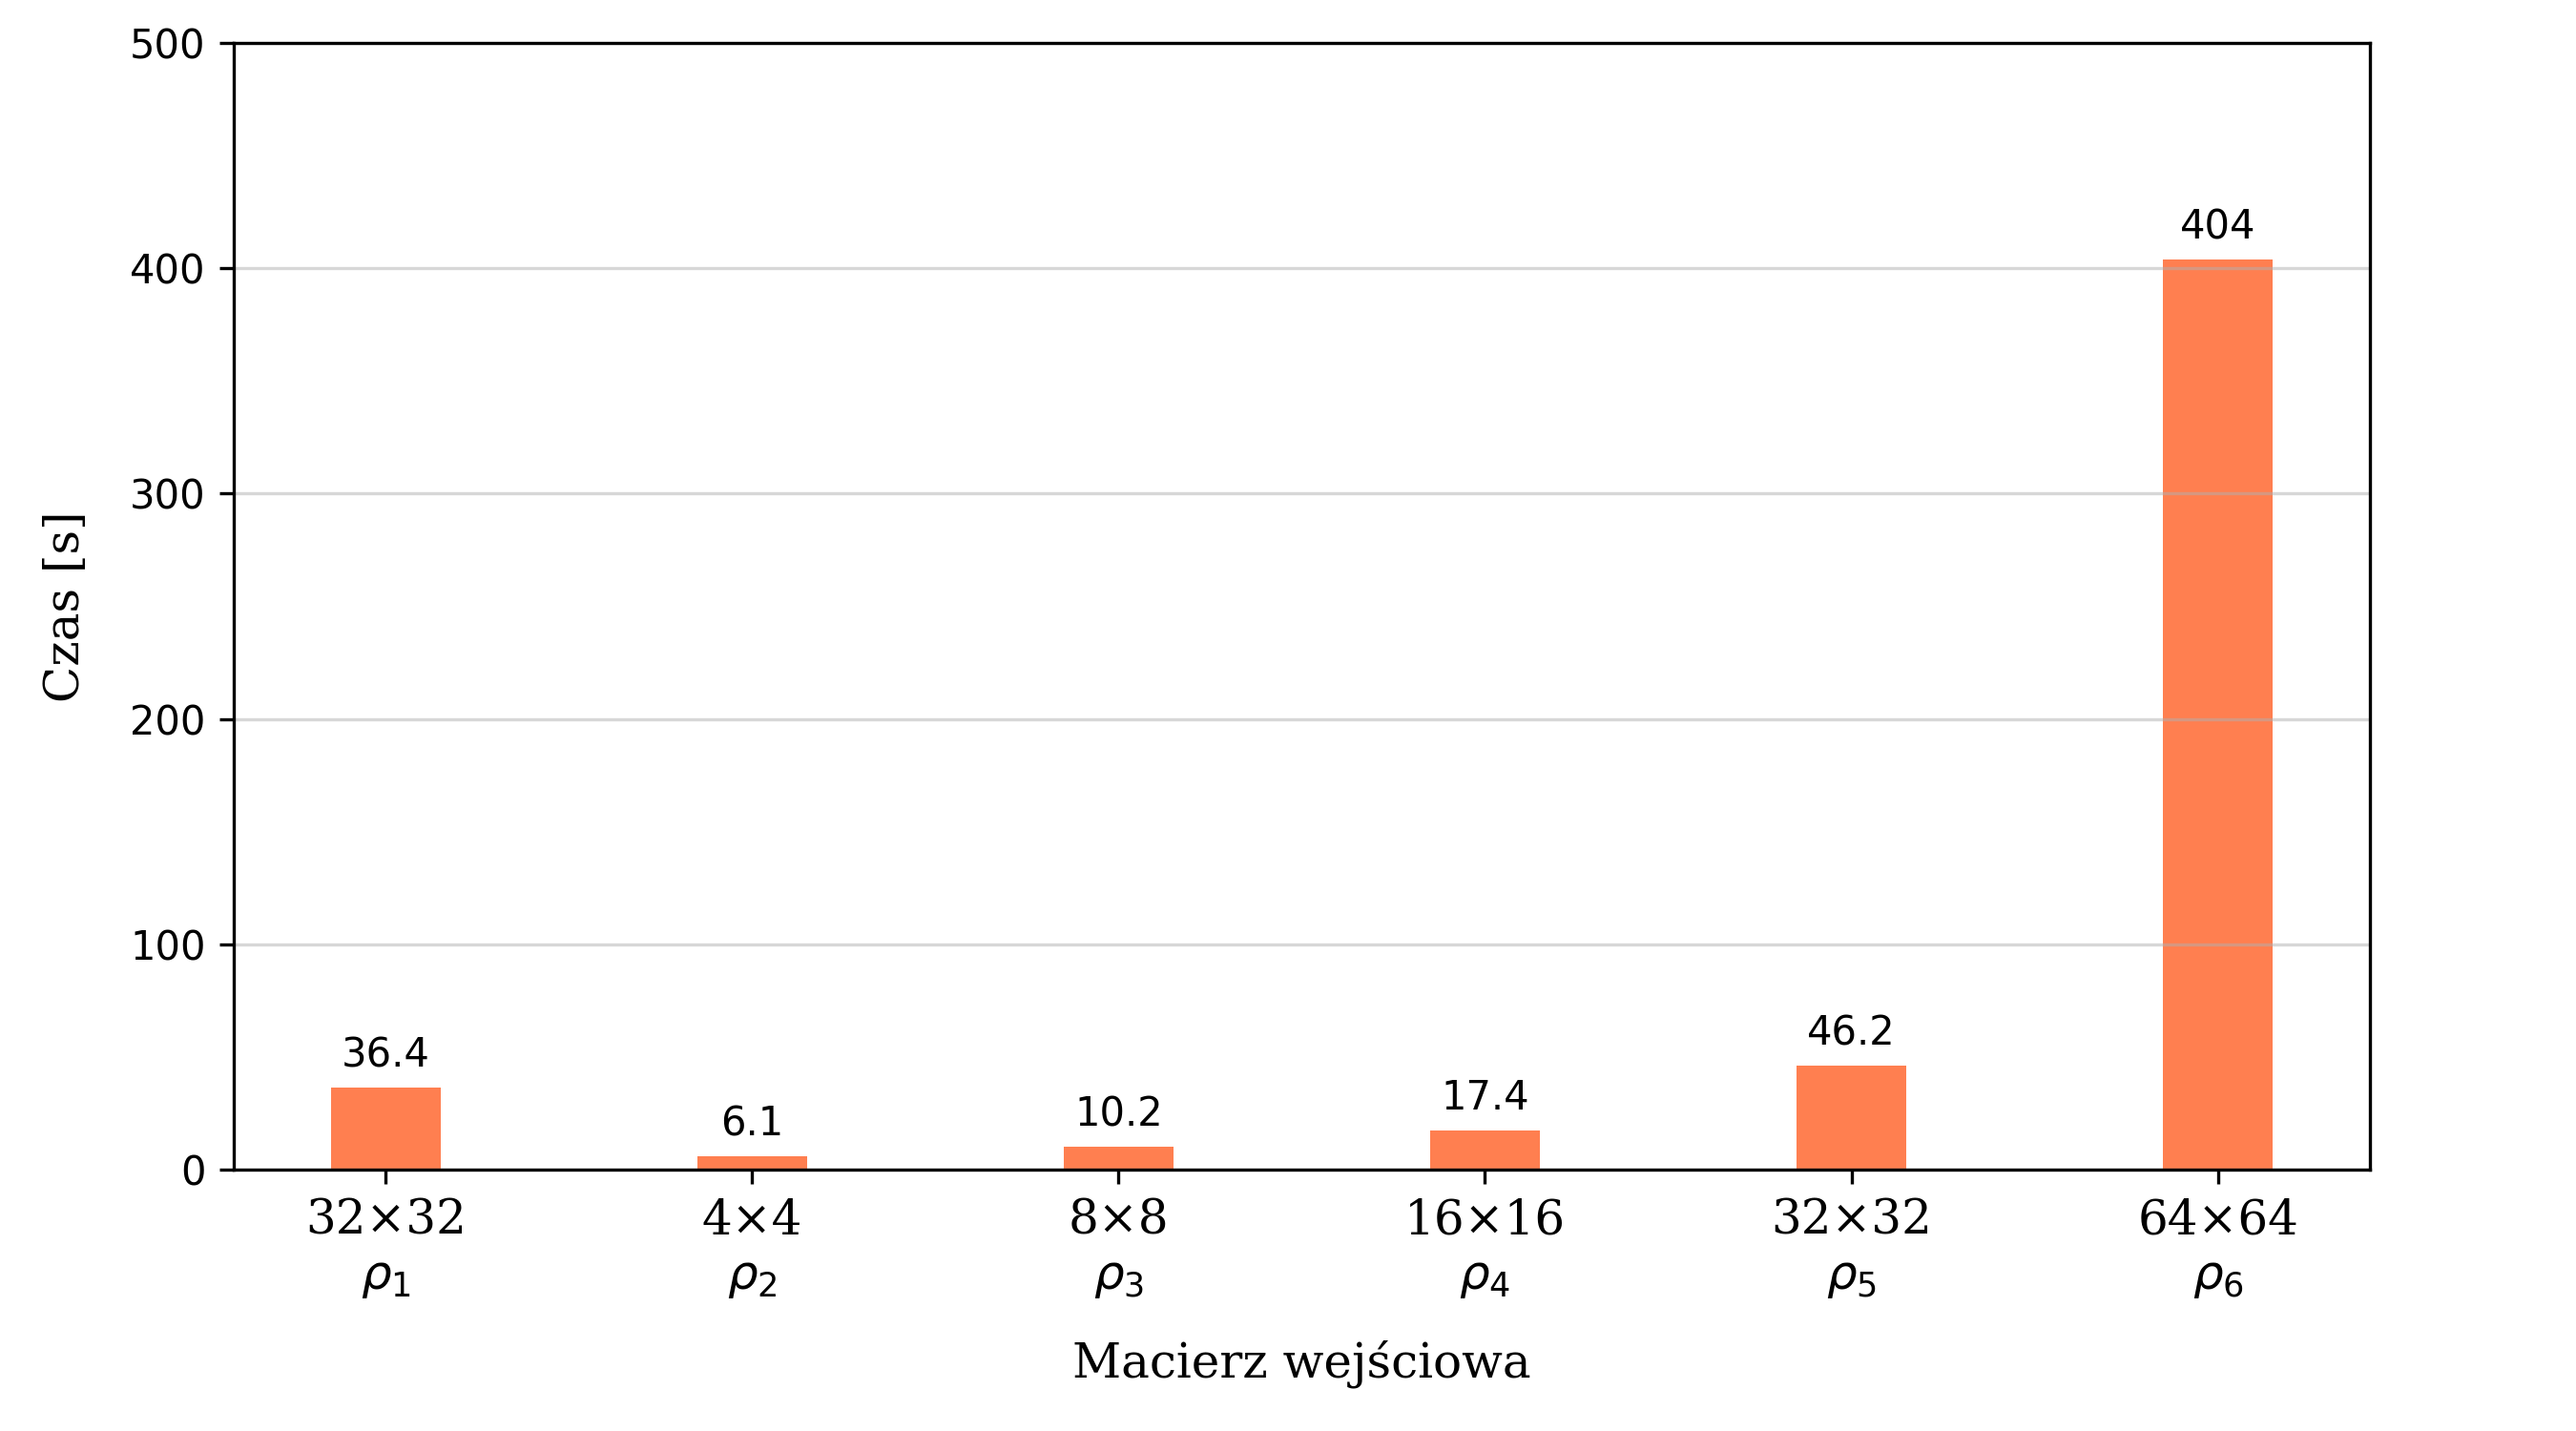
\includegraphics[width=1.0\textwidth]{"resources/original_performance_tests.png"}
      \caption{Wyniki wstępnych testów wydajności oryginalnego kodu dla macierzy $\rho_{1}$ - $\rho
      _{6}$.}
      \label{pre-perf}
    \end{figure}
    \FloatBarrier

    Podczas testów zaobserwowałem interesujące zjawisko dotyczące wydajności dla
    macierzy $64\times64$. W przypadku takich rozmiarów danych biblioteka NumPy automatycznie
    decyduje o wykorzystaniu wielowątkowej implementacji mnożenia macierzowego. Niestety,
    daje to efekt odwrotny do zamierzonego - obliczenia zamiast przyspieszać zwalniają.
    Na rysunku \ref{pre-perf} zostały przedstawione czasy obliczeń dla macierzy
    $\rho_{1}$ - $\rho_{6}$ z domyślnym zachowaniem biblioteki.

    \FloatBarrier
    \begin{figure}[ht]
      \centering
      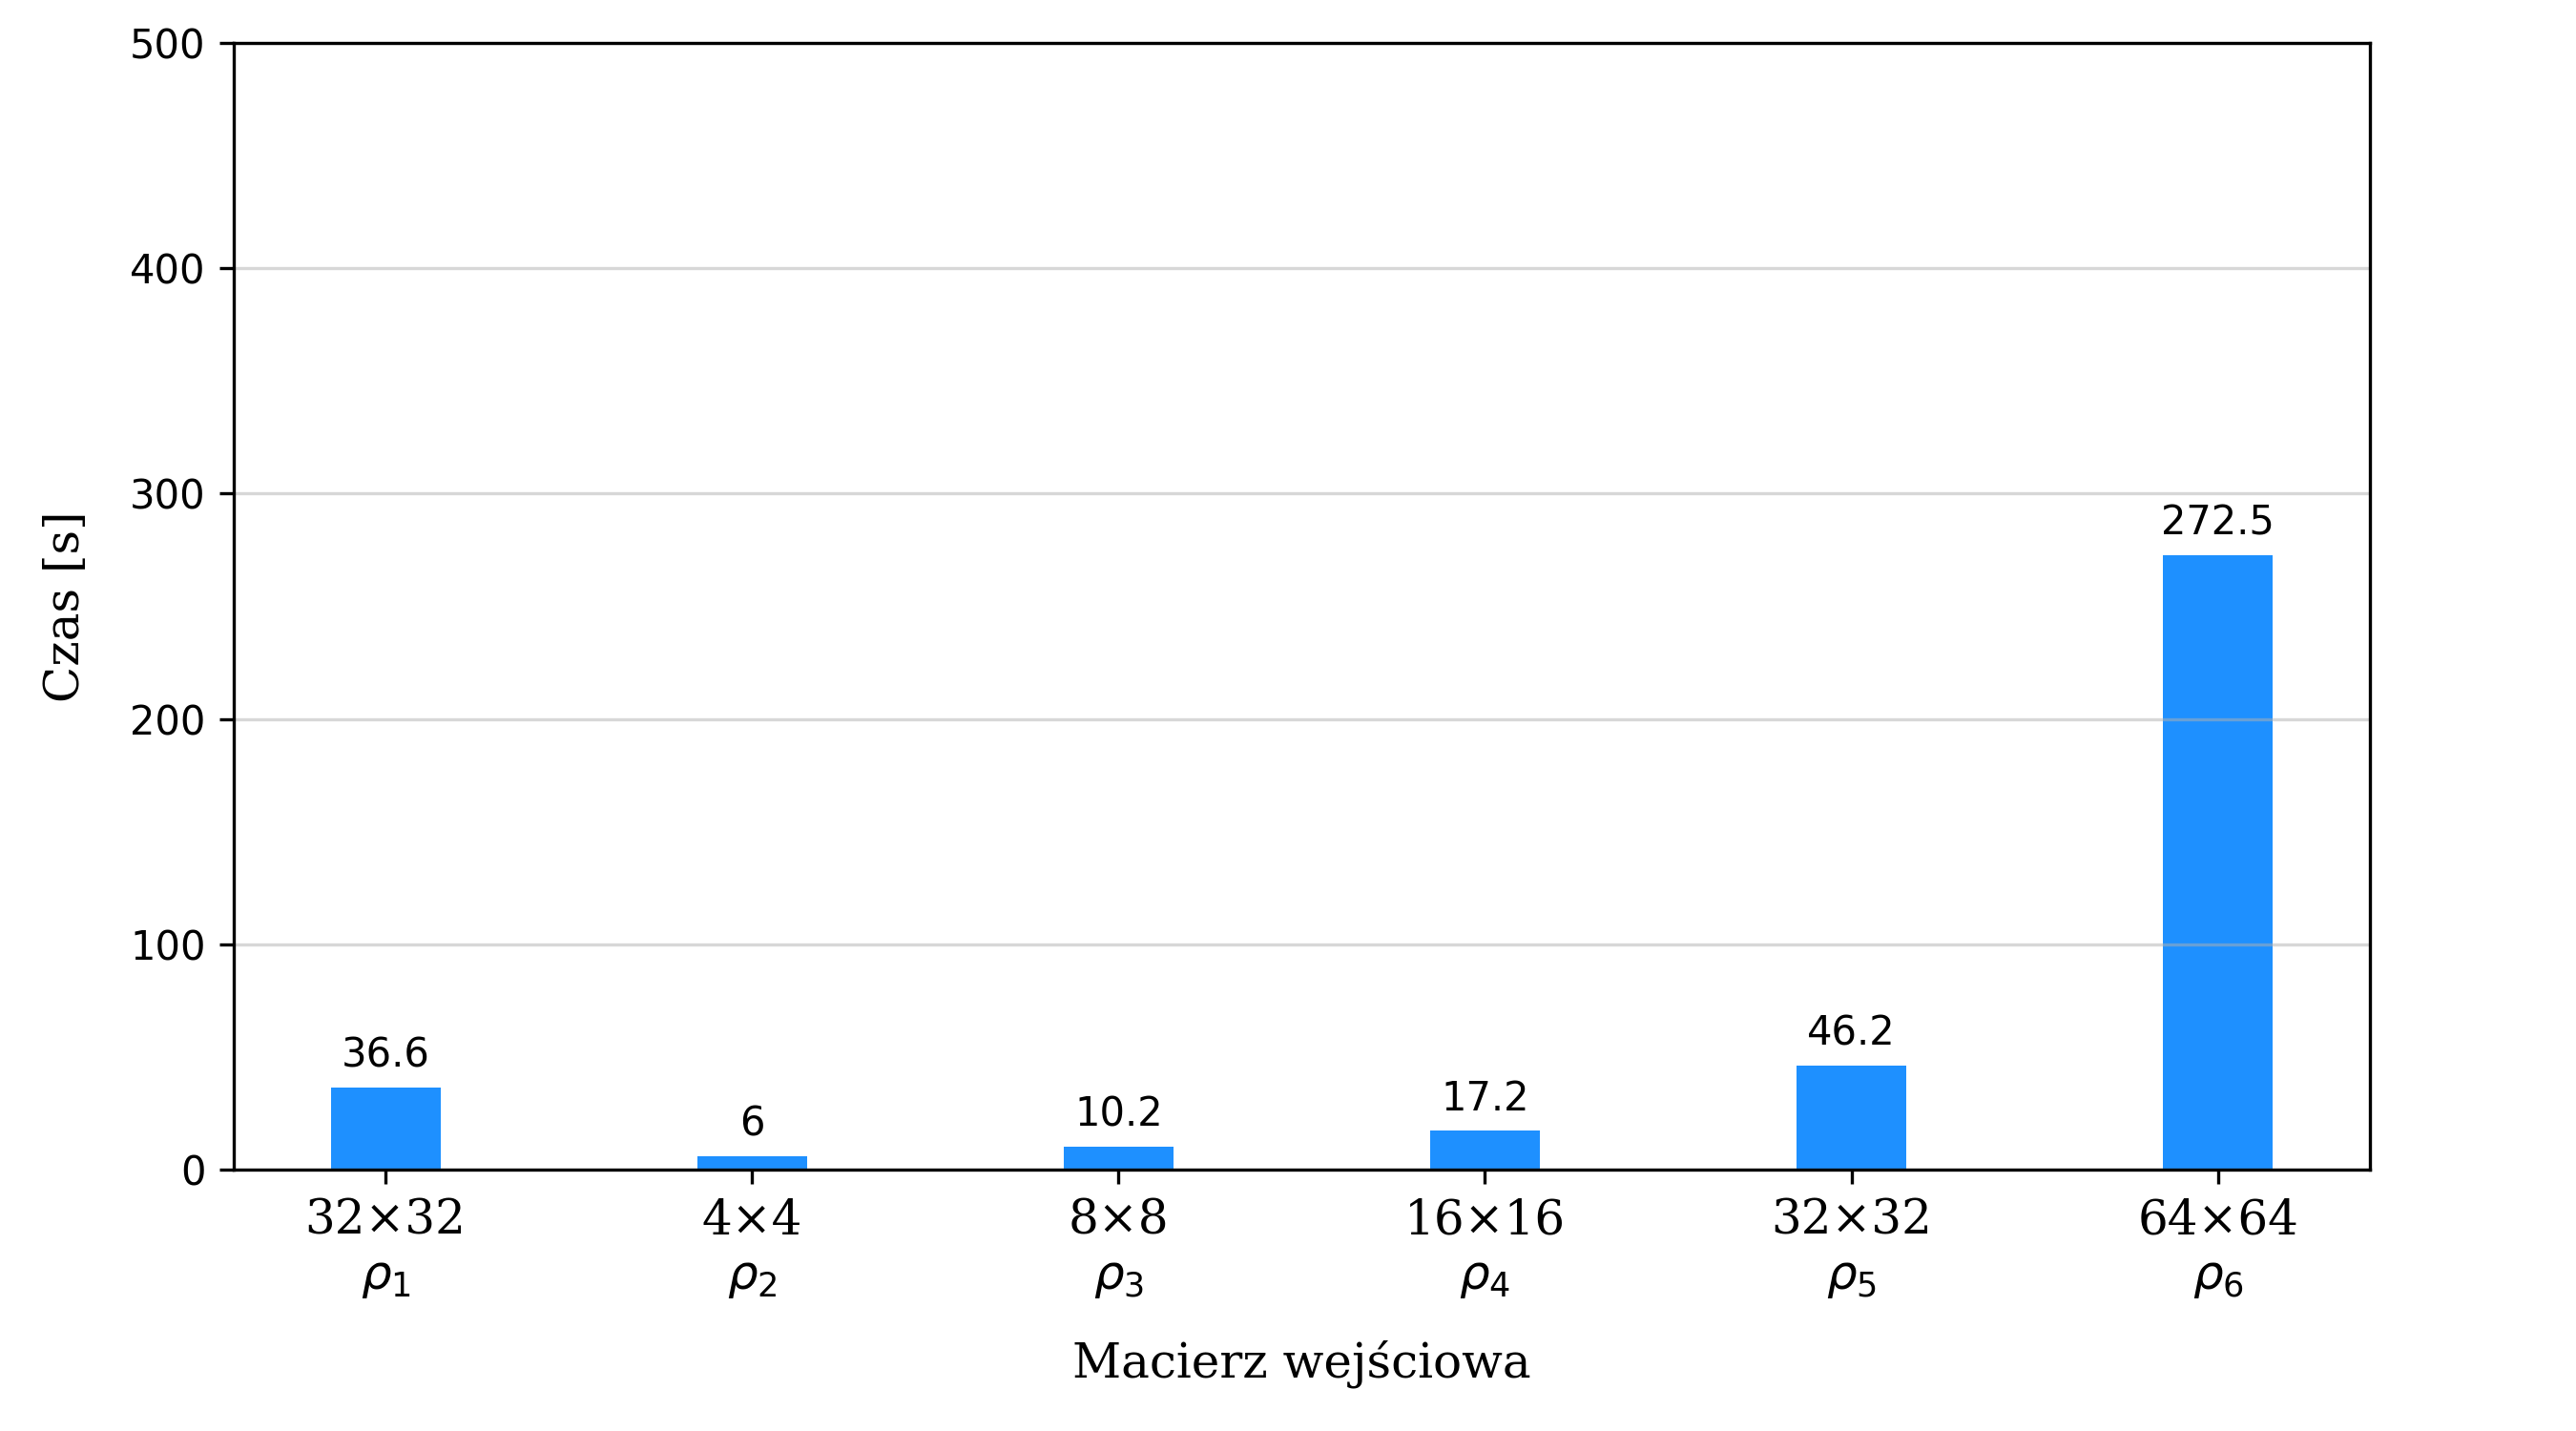
\includegraphics
      [width=1.0\textwidth]{"resources/original_performance_tests_locked.png"}
      \caption{Wyniki wstępnych testów wydajności oryginalnego kodu z zablokowaną liczbą wątków obliczeniowych dla macierzy $\rho
      _{1}$ - $\rho_{6}$.}
      \label{pre-perf-locked}
    \end{figure}
    \FloatBarrier

    Jeśli przy pomocy zmiennych środowiskowych ustawimy ilość wątków wykorzystywanych do
    obliczeń na 1 uzyskujemy znaczące skrócenie czasu obliczeń dla macierzy $64\times64$.
    Wyniki testów w takich warunkach zostały przedstawione na rysunku
    \ref{pre-perf-locked}. Dla macierzy w mniejszych rozmiarach nie odnotowałem różnicy w
    wydajności pomiędzy konfiguracją domyślną, a manualnie dostosowywaną. Warto dodać że
    ilość iteracji wykonywanych przez program nie zmienia się, różnica wynika wyłącznie
    z czasu trwania operacji arytmetycznych. Taki stan rzeczy najprawdopodobniej jest wynikiem
    dodatkowego obciążenia ze strony komunikacji i/lub synchronizacji między wątkami.

    Chciałbym uściślić, że w dalszej części pracy, mówiąc o wynikach oryginalnego kodu,
    będę miał na myśli wersję bez zablokowanej ilości wątków, a więc tę której wyniki umieszczone
    są na rysunku \ref{pre-perf}, jako że to była pierwotna postać kodu, natomiast zablokowanie
    ilości wątków wymagało już jego modyfikacji.

    \subsection{Pomiary z podwójną precyzją}
    W dalszej części pracy prezentuje wyniki pomiarów czasu pracy re-implementacji algorytmu
    QGA wykorzystujących liczby zmiennoprzecinkowe podwójnej precyzji.

    \subsubsection{ Python i NumPy }
    Pomiary czasu pracy były wykonywane przy użyciu macierzy $\rho_{1}$ - $\rho_{6}$.
    Dane przekazywałem kolejno do programu z poleceniem działania w trybie FSnQd\footnote{Tryb
    FSnQd jest odpowiednikiem trybu 1 (full separability of an n-quDit state) z oryginalnego
    kodu.} do osiągnięcia co najmniej 1000 korekcji lub do 2.000.000 iteracji algorytmu,
    w zależności od tego co nastąpi szybciej. Dla wszystkich macierzy algorytm uzyskał
    co najmniej 1000 korekcji i w żadnym przypadku nie osiągnął maksymalnej liczby
    iteracji. Dla każdej macierzy pomiar był powtarzany pięciokrotnie a wyniki zostały uśrednione.
    Podczas obliczeń ziarno domyślnego globalnego generatora liczb losowych biblioteki
    NumPy było ustawione na 0. Program działał z zablokowaną liczbą wątków
    obliczeniowych. Pomiary czasu pracy dotyczyły przede wszystkim samego algorytmu\footnote{Pomiary
    nie biorą więc pod uwagę czasu pochłoniętego przez importowanie modułów itp.,
    natomiast operacje wczytywania danych i pisania do plików są wliczane w czas pracy, ponieważ
    wbudowany w program mechanizm pomiaru czasu pracy rozpoczyna pomiar zanim dane zostaną
    załadowane.}.

    \begin{figure}[ht]
      \centering
      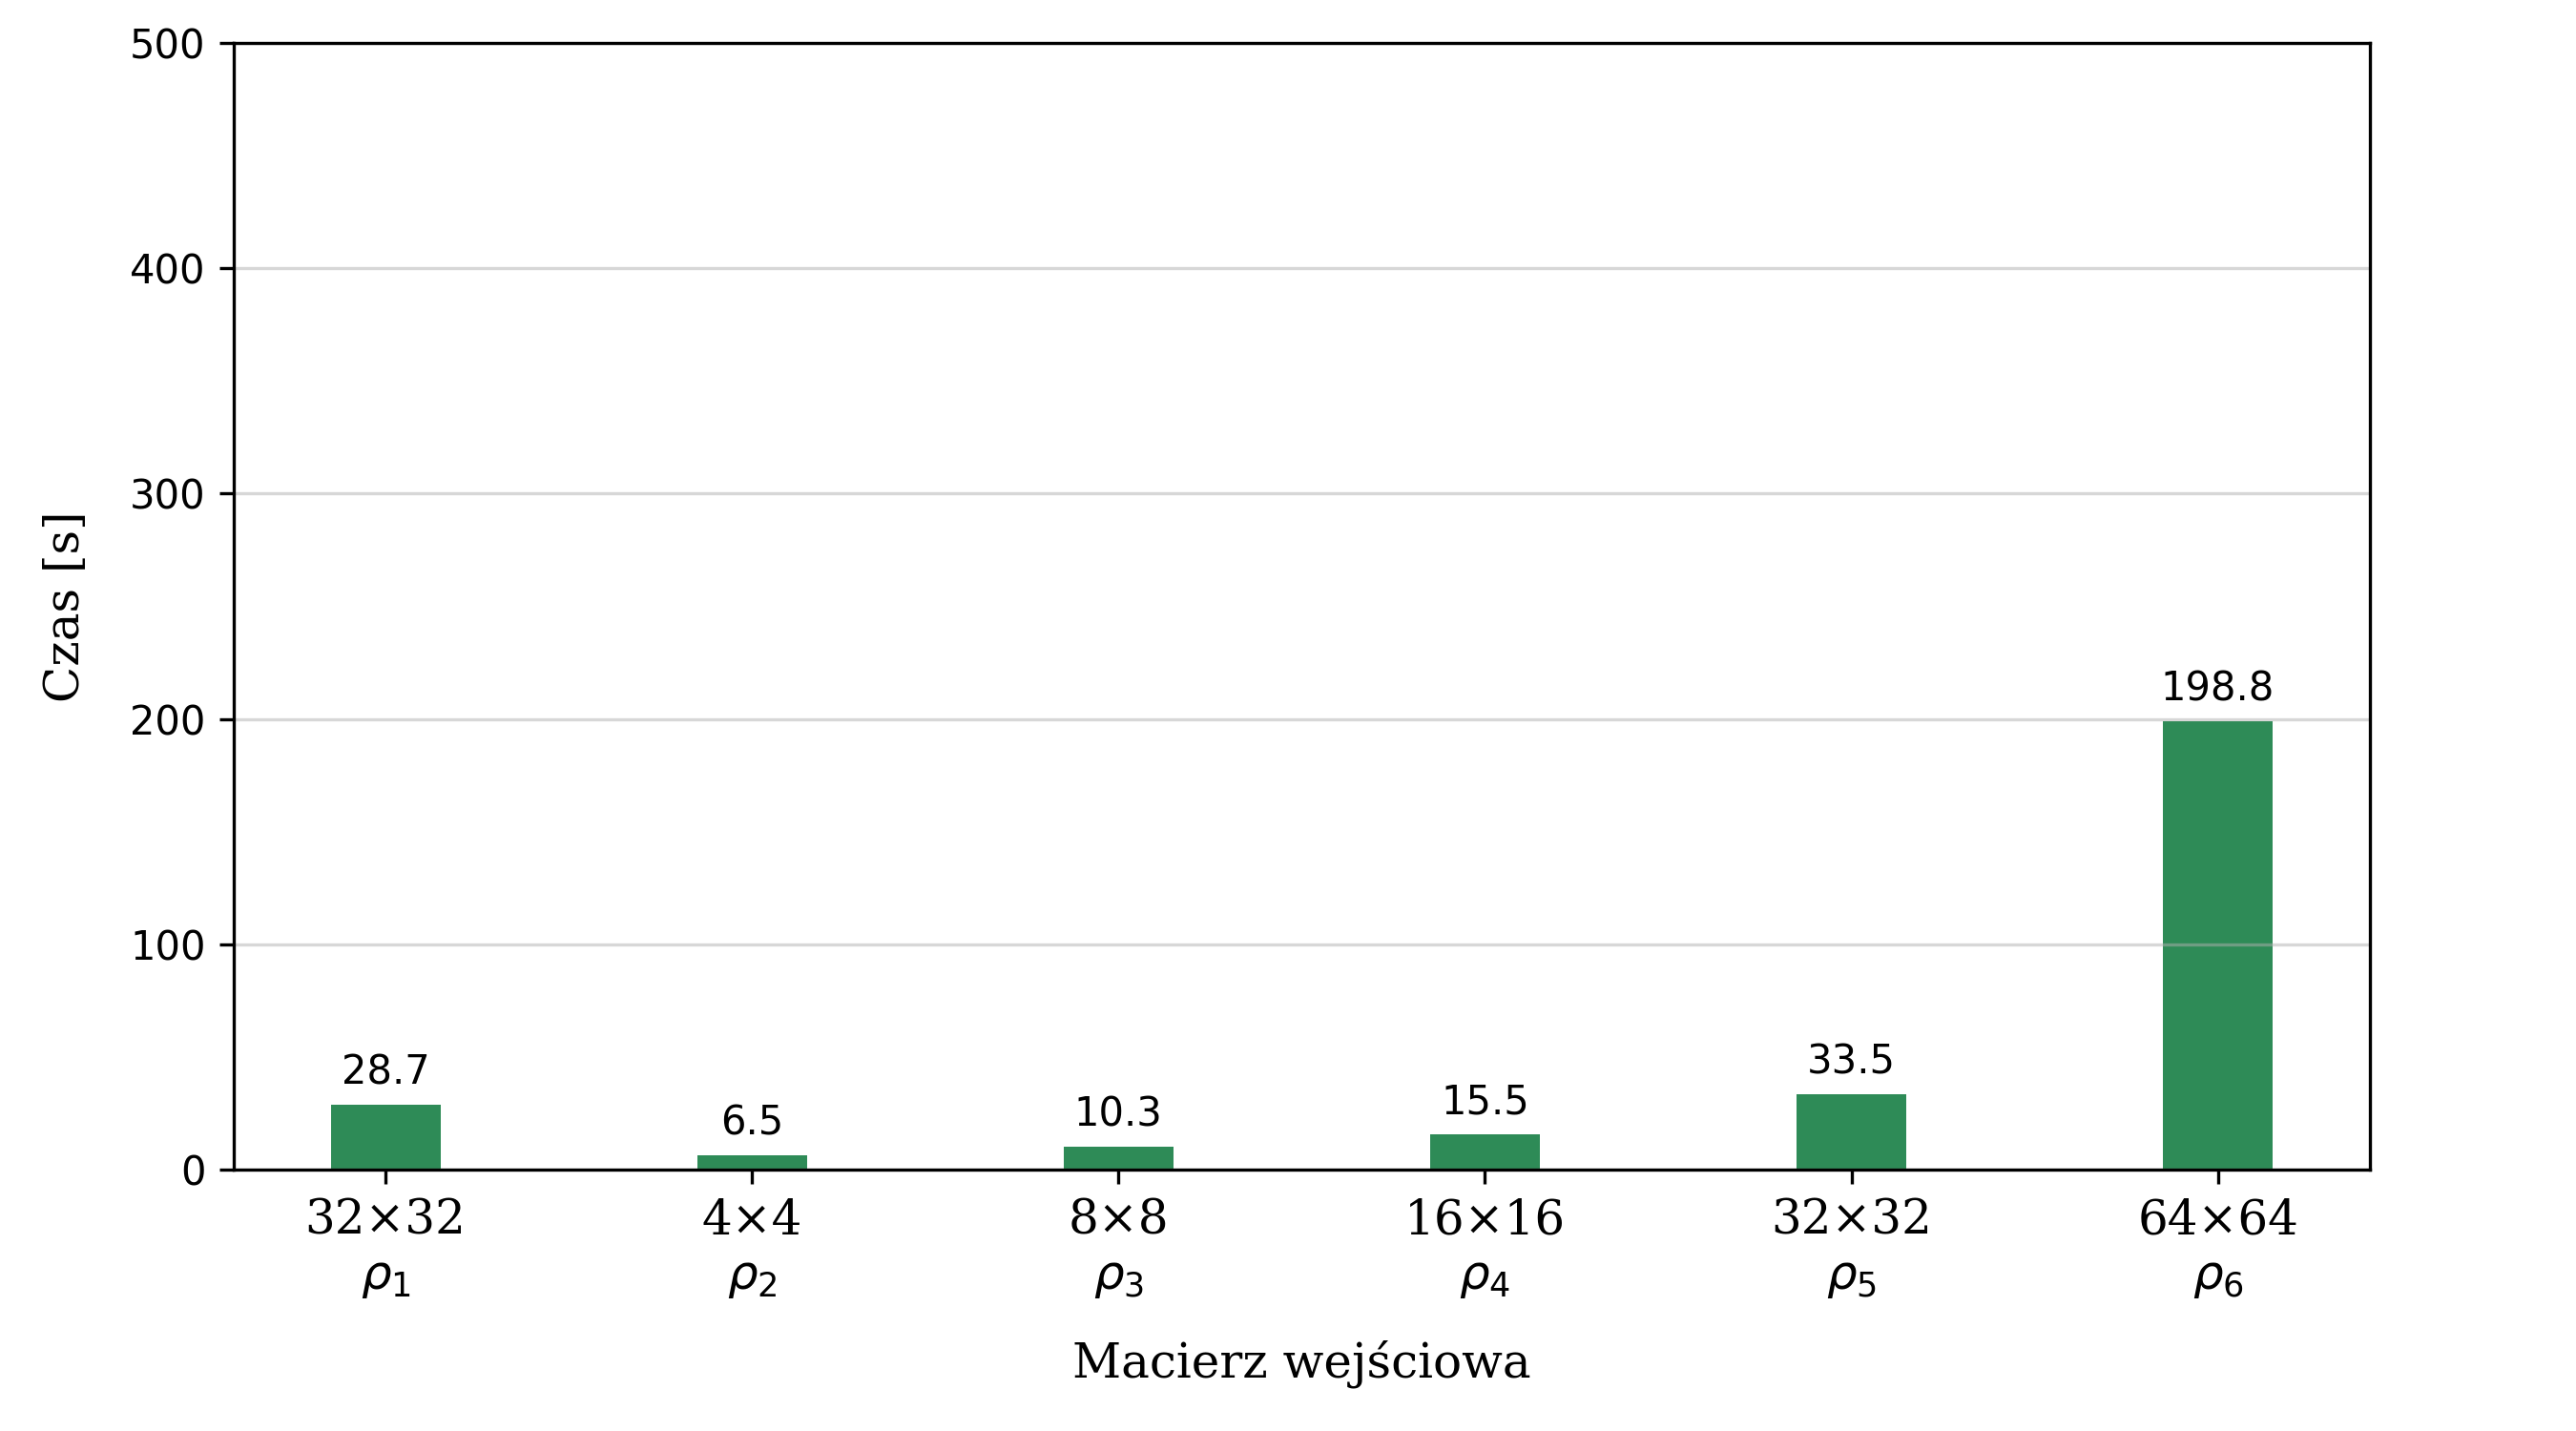
\includegraphics
      [width=1.0\textwidth]{"resources/python_and_numpy_performance_tests.png"}
      \caption{Wyniki testów wydajności alternatywnej implementacji Python z użyciem biblioteki NumPy dla macierzy $\rho
      _{1}$ - $\rho_{6}$.}
      \label{python-numpy-double-precision}
    \end{figure}

    Uzyskane wyniki zostały przedstawione na rysunku \ref{python-numpy-double-precision}.
    W przypadku małych macierzy wyniki są bardzo zbliżone, natomiast w przypadku
    macierzy $32\times32$ i $64\times64$ występuje znacząca poprawa wydajności, odpowiednio
    $7.9s$ ($\approx 21\%$) dla $\rho_{1}$, $12.7s$ ($\approx 27\%$) dla $\rho_{5}$ i
    $20 5.2s$ ($\approx 50\%$) dla $\rho_{6}$.

    \FloatBarrier

    \subsubsection{ Python i NumPy z AOT }
    Pomiary czasu pracy były wykonywane w taki sam sposób jak dla implementacji bez AOT.

    \begin{figure}[ht]
      \centering
      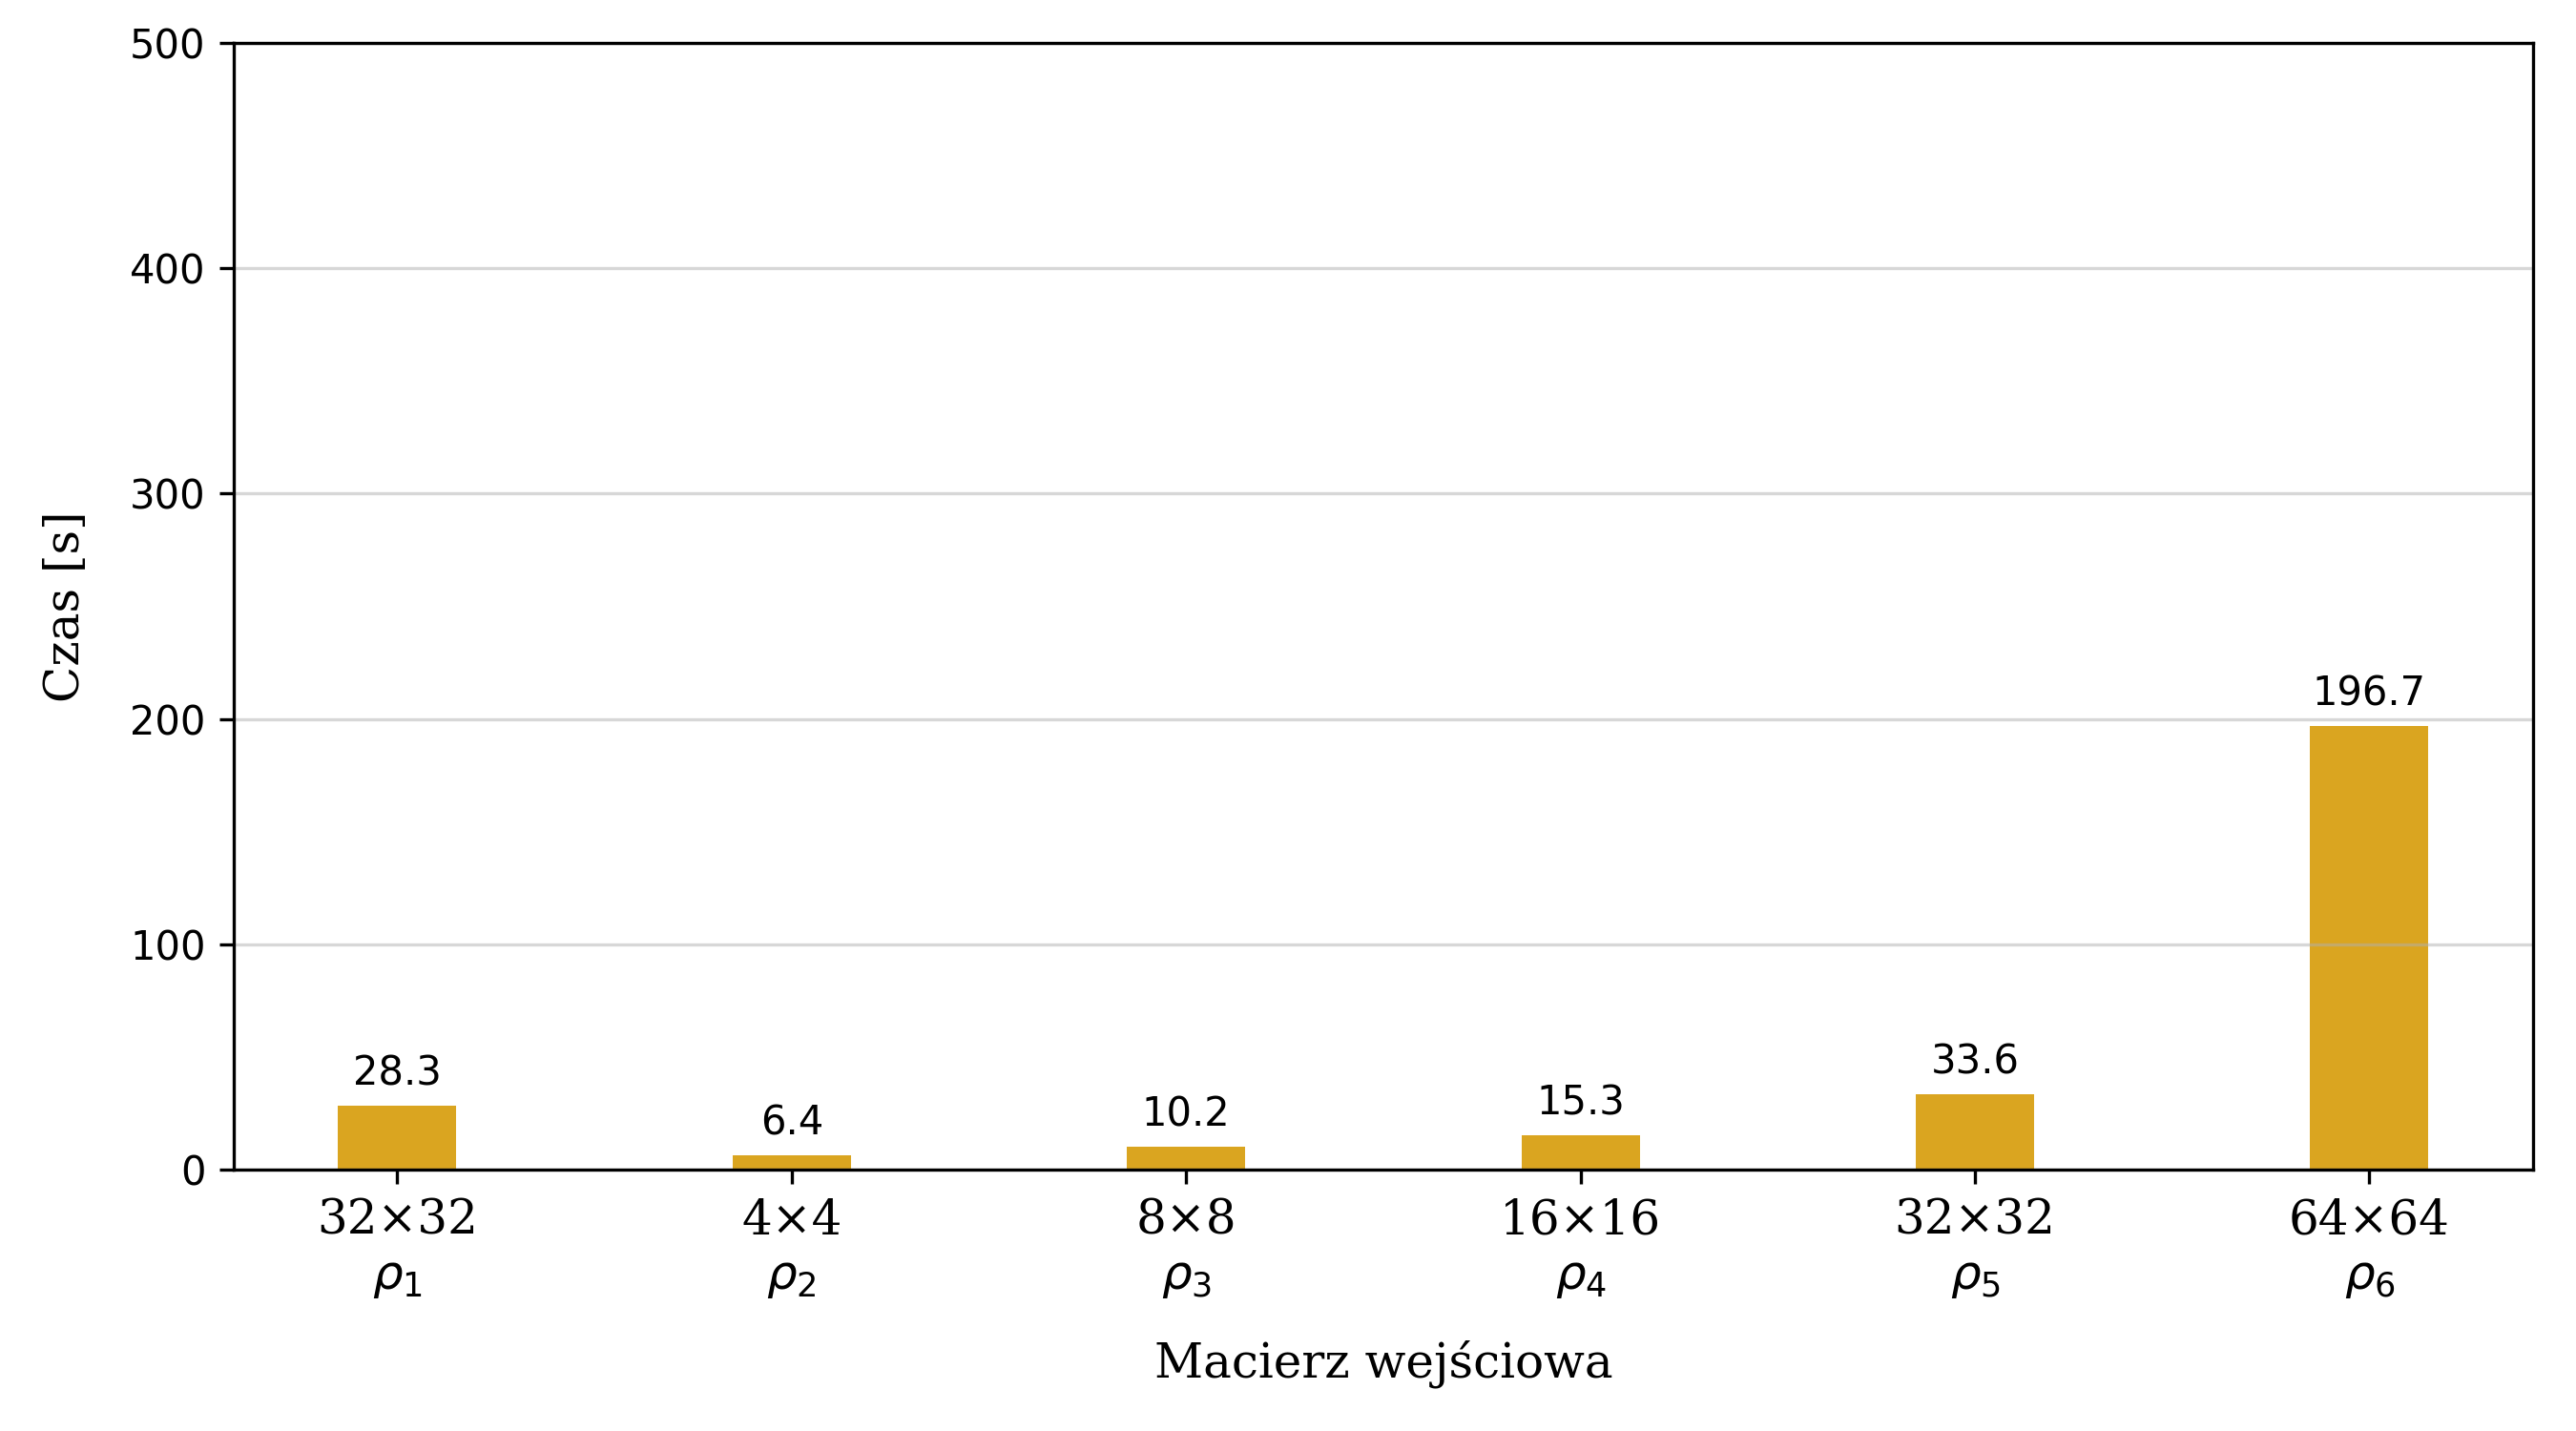
\includegraphics
      [width=1.0\textwidth]{"resources/python_and_numpy_and_aot_performance_tests.png"}
      \caption{Wyniki testów wydajności implementacji Python z użyciem biblioteki NumPy oraz pakietu Cython do kompilacji AOT dla macierzy $\rho
      _{1}$ - $\rho_{6}$.}
      \label{python-numpy-aot-double-precision}
    \end{figure}

    Na rysunku \ref{python-numpy-aot-double-precision} przedstawione zostały wyniki
    pomiarów czasu pracy skompilowanej wersji w języku Python bazującej na bibliotece
    NumPy wykorzystujące macierze $\rho_{1}$ - $\rho_{6}$. kompilacja nie poskutkowała istotnym
    skróceniem czasu pracy programu względem wariantu bez AOT, różnice wynoszą koło 1\%.
    Uzysk ten może być spowodowany usunięciem szczątkowego obciążenia ze strony
    interpretera, które nie jest mierzalne podczas krótszych testów z mniejszymi macierzami.
    Możliwe jest również że ta różnica wynika z korzystniejszych warunków losowo
    zapewnionych przez system operacyjny.

    \FloatBarrier

    \subsubsection{ Python i NumPy z JIT }
    Pomiary czasu pracy były wykonywane w taki sam sposób jak dla implementacji bez JIT.

    \begin{figure}[ht]
      \centering
      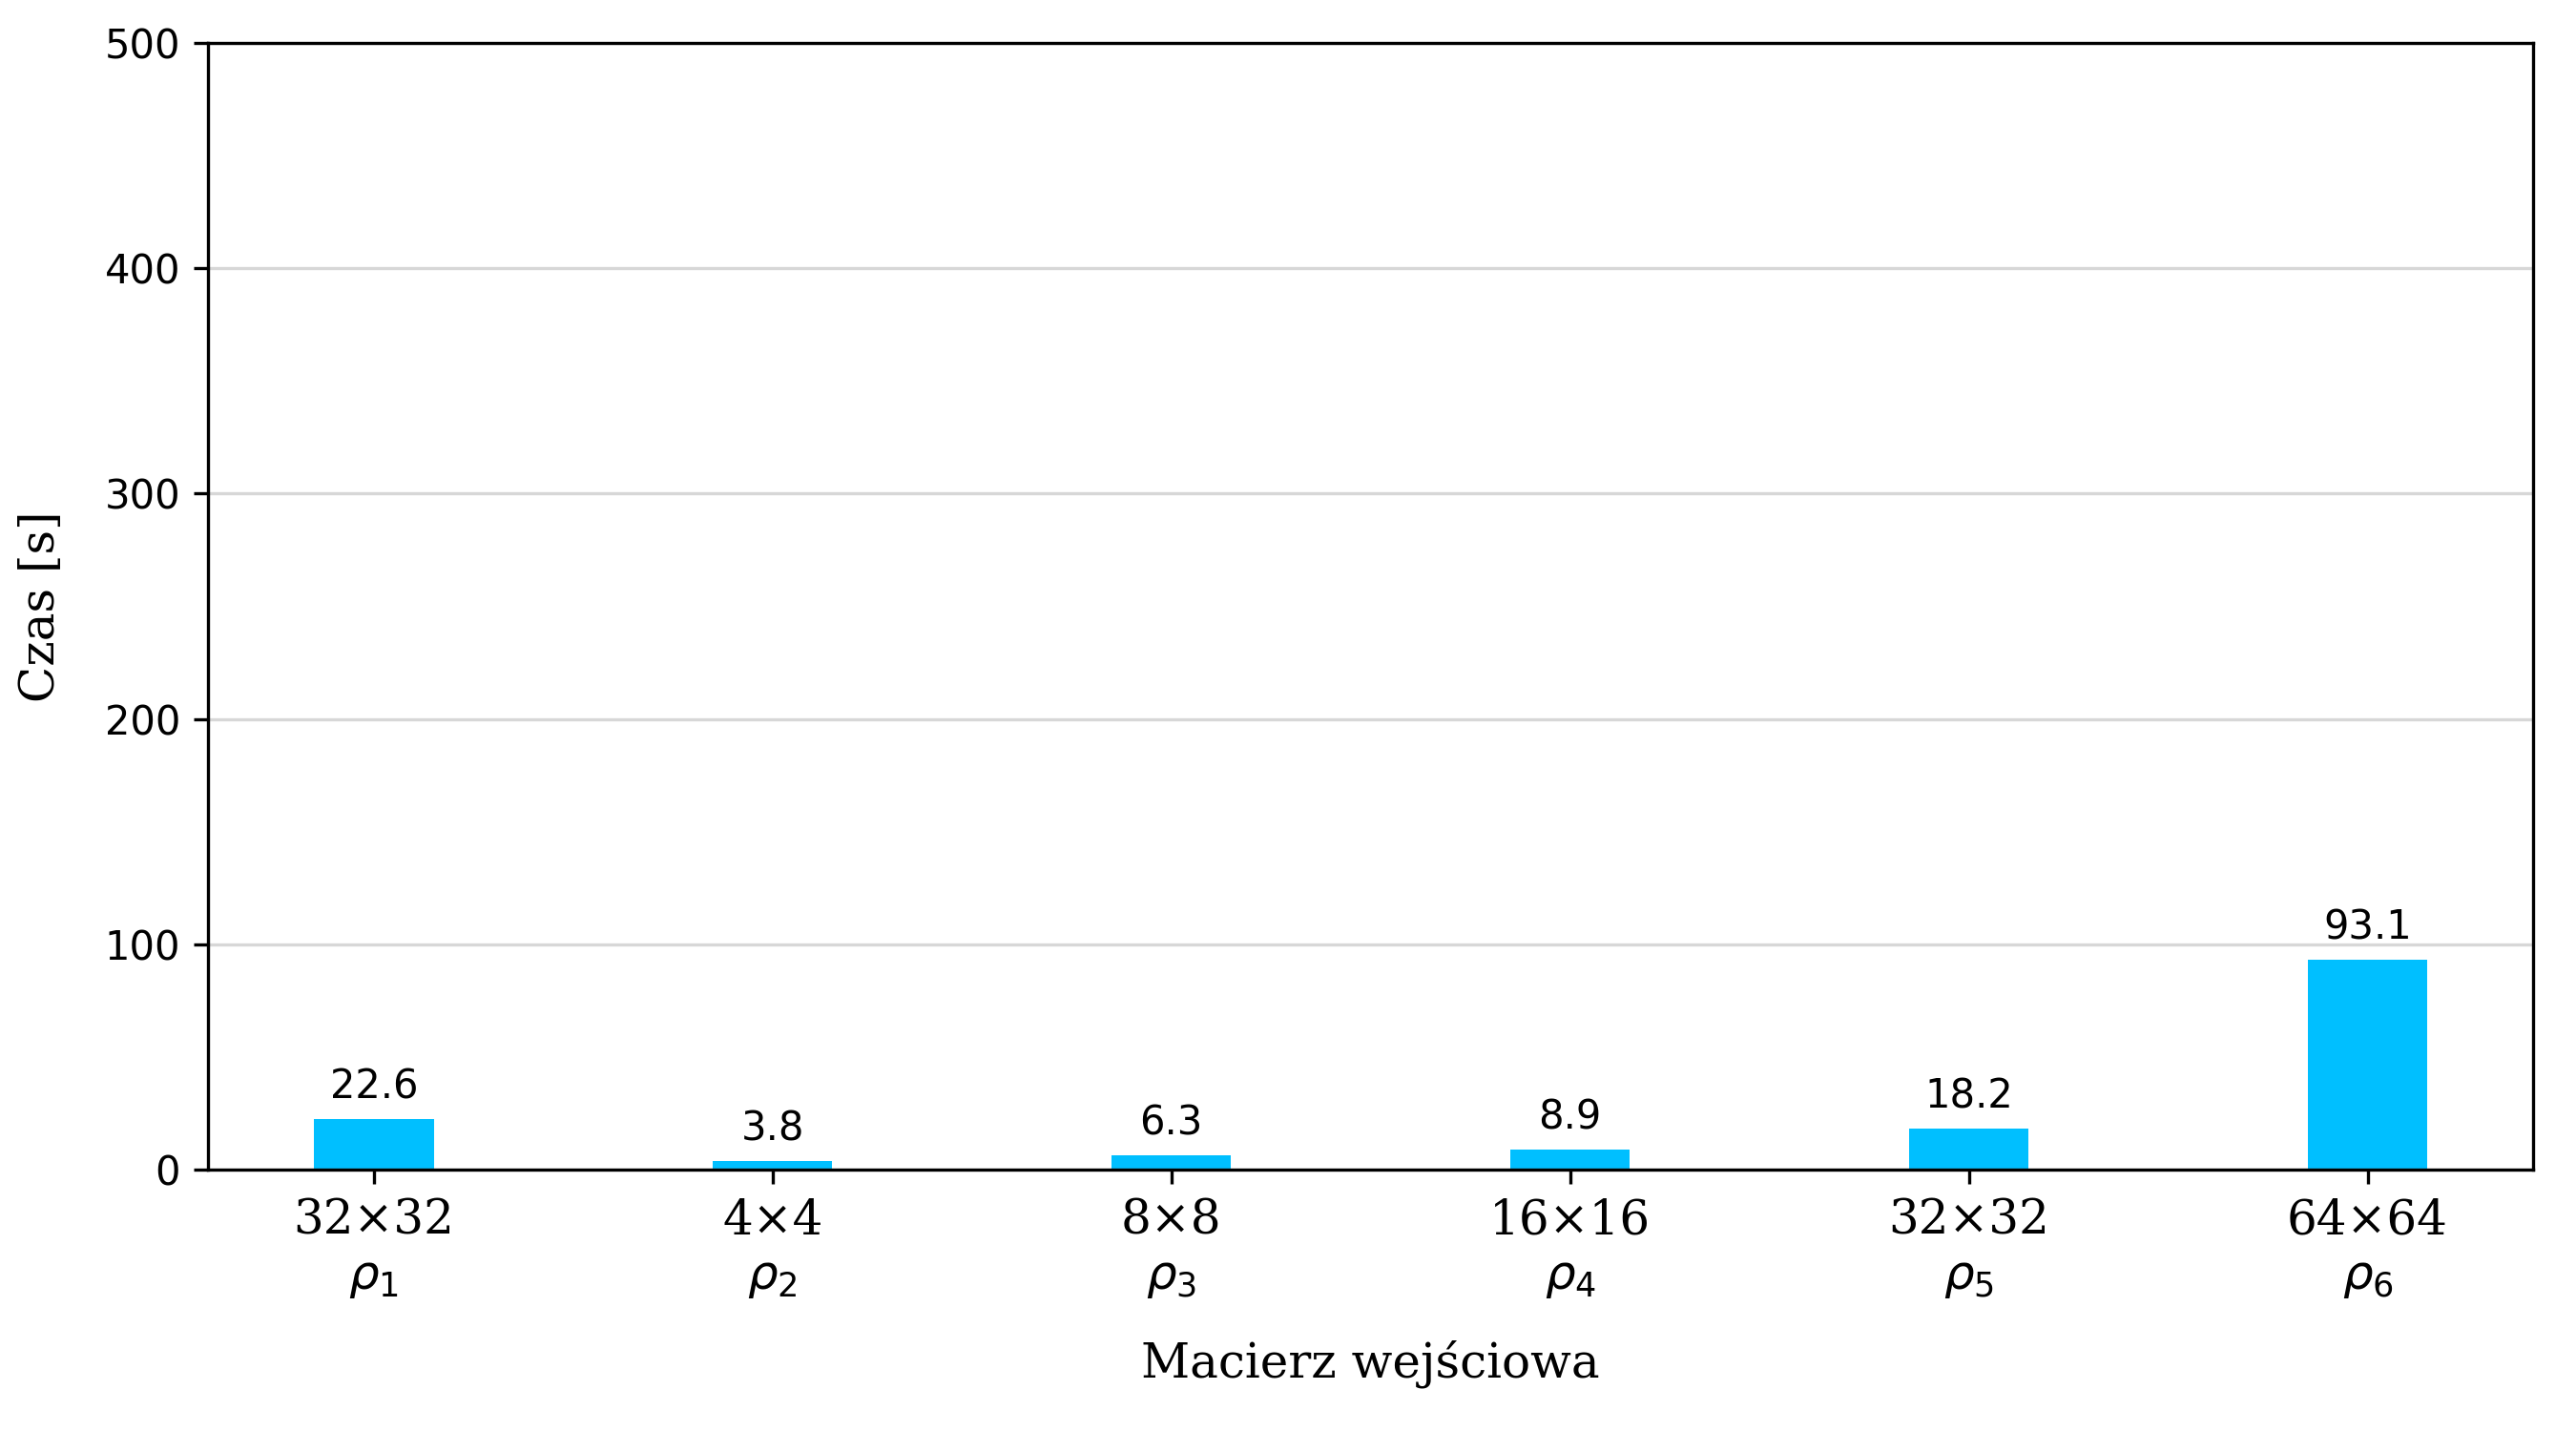
\includegraphics
      [width=1.0\textwidth]{"resources/python_and_numpy_and_jit_performance_tests.png"}
      \caption{Wyniki testów wydajności implementacji w języku Python z użyciem biblioteki NumPy i pakietu Numba do kompilacji JIT dla macierzy $\rho
      _{1}$ - $\rho_{6}$.}
      \label{python-numpy-jit-double-precision}
    \end{figure}

    Na rysunku \ref{python-numpy-jit-double-precision} przedstawione zostały wyniki
    uzyskane podczas pomiarów czasu pracy implementacji z kompilacją JIT wykonywaną przy
    pomocy biblioteki Numba, wykorzystując macierze $\rho_{1}$ - $\rho_{6}$.
    Implementacja ta oferowała podczas testów blisko dwukrotnie krótszy czas obliczeń, względem
    oryginału, w przypadku macierzy mniejszych niż $32\times32$. Dla macierzy większych uzysk
    wynosił odpowiednio $13.8s$ ($\approx 38\%$) dla $\rho_{1}$, $28s$ ($\approx 60\%$)
    dla $\rho_{5}$ i $310 .9s$ ($\approx 77\%$) dla $\rho_{6}$.

    Tak znaczącą poprawę implementacja zawdzięcza prawdopodobnie temu, że kompilator JIT
    całkowicie pozbywa się obciążenia ze strony dynamicznego systemu typów, generując
    wyspecjalizowany statycznie typowany kod maszynowy. Ponadto może on specjalizować kod
    dla dokładnie jednej platformy, korzystając z całego spektrum jej możliwości. Dotyczy
    to na przykład instrukcji SIMD, takich jak AVX2 i FMA, które są dostępne w procesorze
    użytym do testów, ale wiele wciąż popularnych procesorów ich nie posiada. Wymusza to,
    przy kompilacji AOT, zastąpienie tych instrukcji innymi szerzej dostępnymi, aby
    zmaksymalizować przenośność kodu. Dodatkowo kompilator może brać pod uwagę inne charakterystyczne
    cechy konkretnych architektur.

    \FloatBarrier

    \subsubsection{ Rust i Ndaray}


    Pomiary czasu pracy implementacji w języku Rust były wykonywane przy użyciu macierzy
    $\rho_{2}$ - $\rho_{6}$. Dane przekazywałem kolejno do programu z poleceniem działania
    w trybie FSnQd do osiągnięcia co najmniej 1000 korekcji lub do 2.000.000 iteracji
    algorytmu, w zależności od tego co nastąpi szybciej. Dla wszystkich macierzy
    algorytm uzyskał co najmniej 1000 korekcji i w żadnym przypadku nie osiągnął
    maksymalnej liczby iteracji. Dla każdej macierzy pomiar był powtarzany pięciokrotnie
    a wyniki zostały uśrednione. Pomiary czasu pracy dotyczyły przede wszystkim samego
    algorytmu\footnote{Nie biorą więc pod uwagę czasu pochłoniętego przez importowanie modułów
    itp., natomiast operacje wczytywania danych i pisania do plików są wliczane w czas pracy.}.

    \begin{figure}[ht]
      \centering
      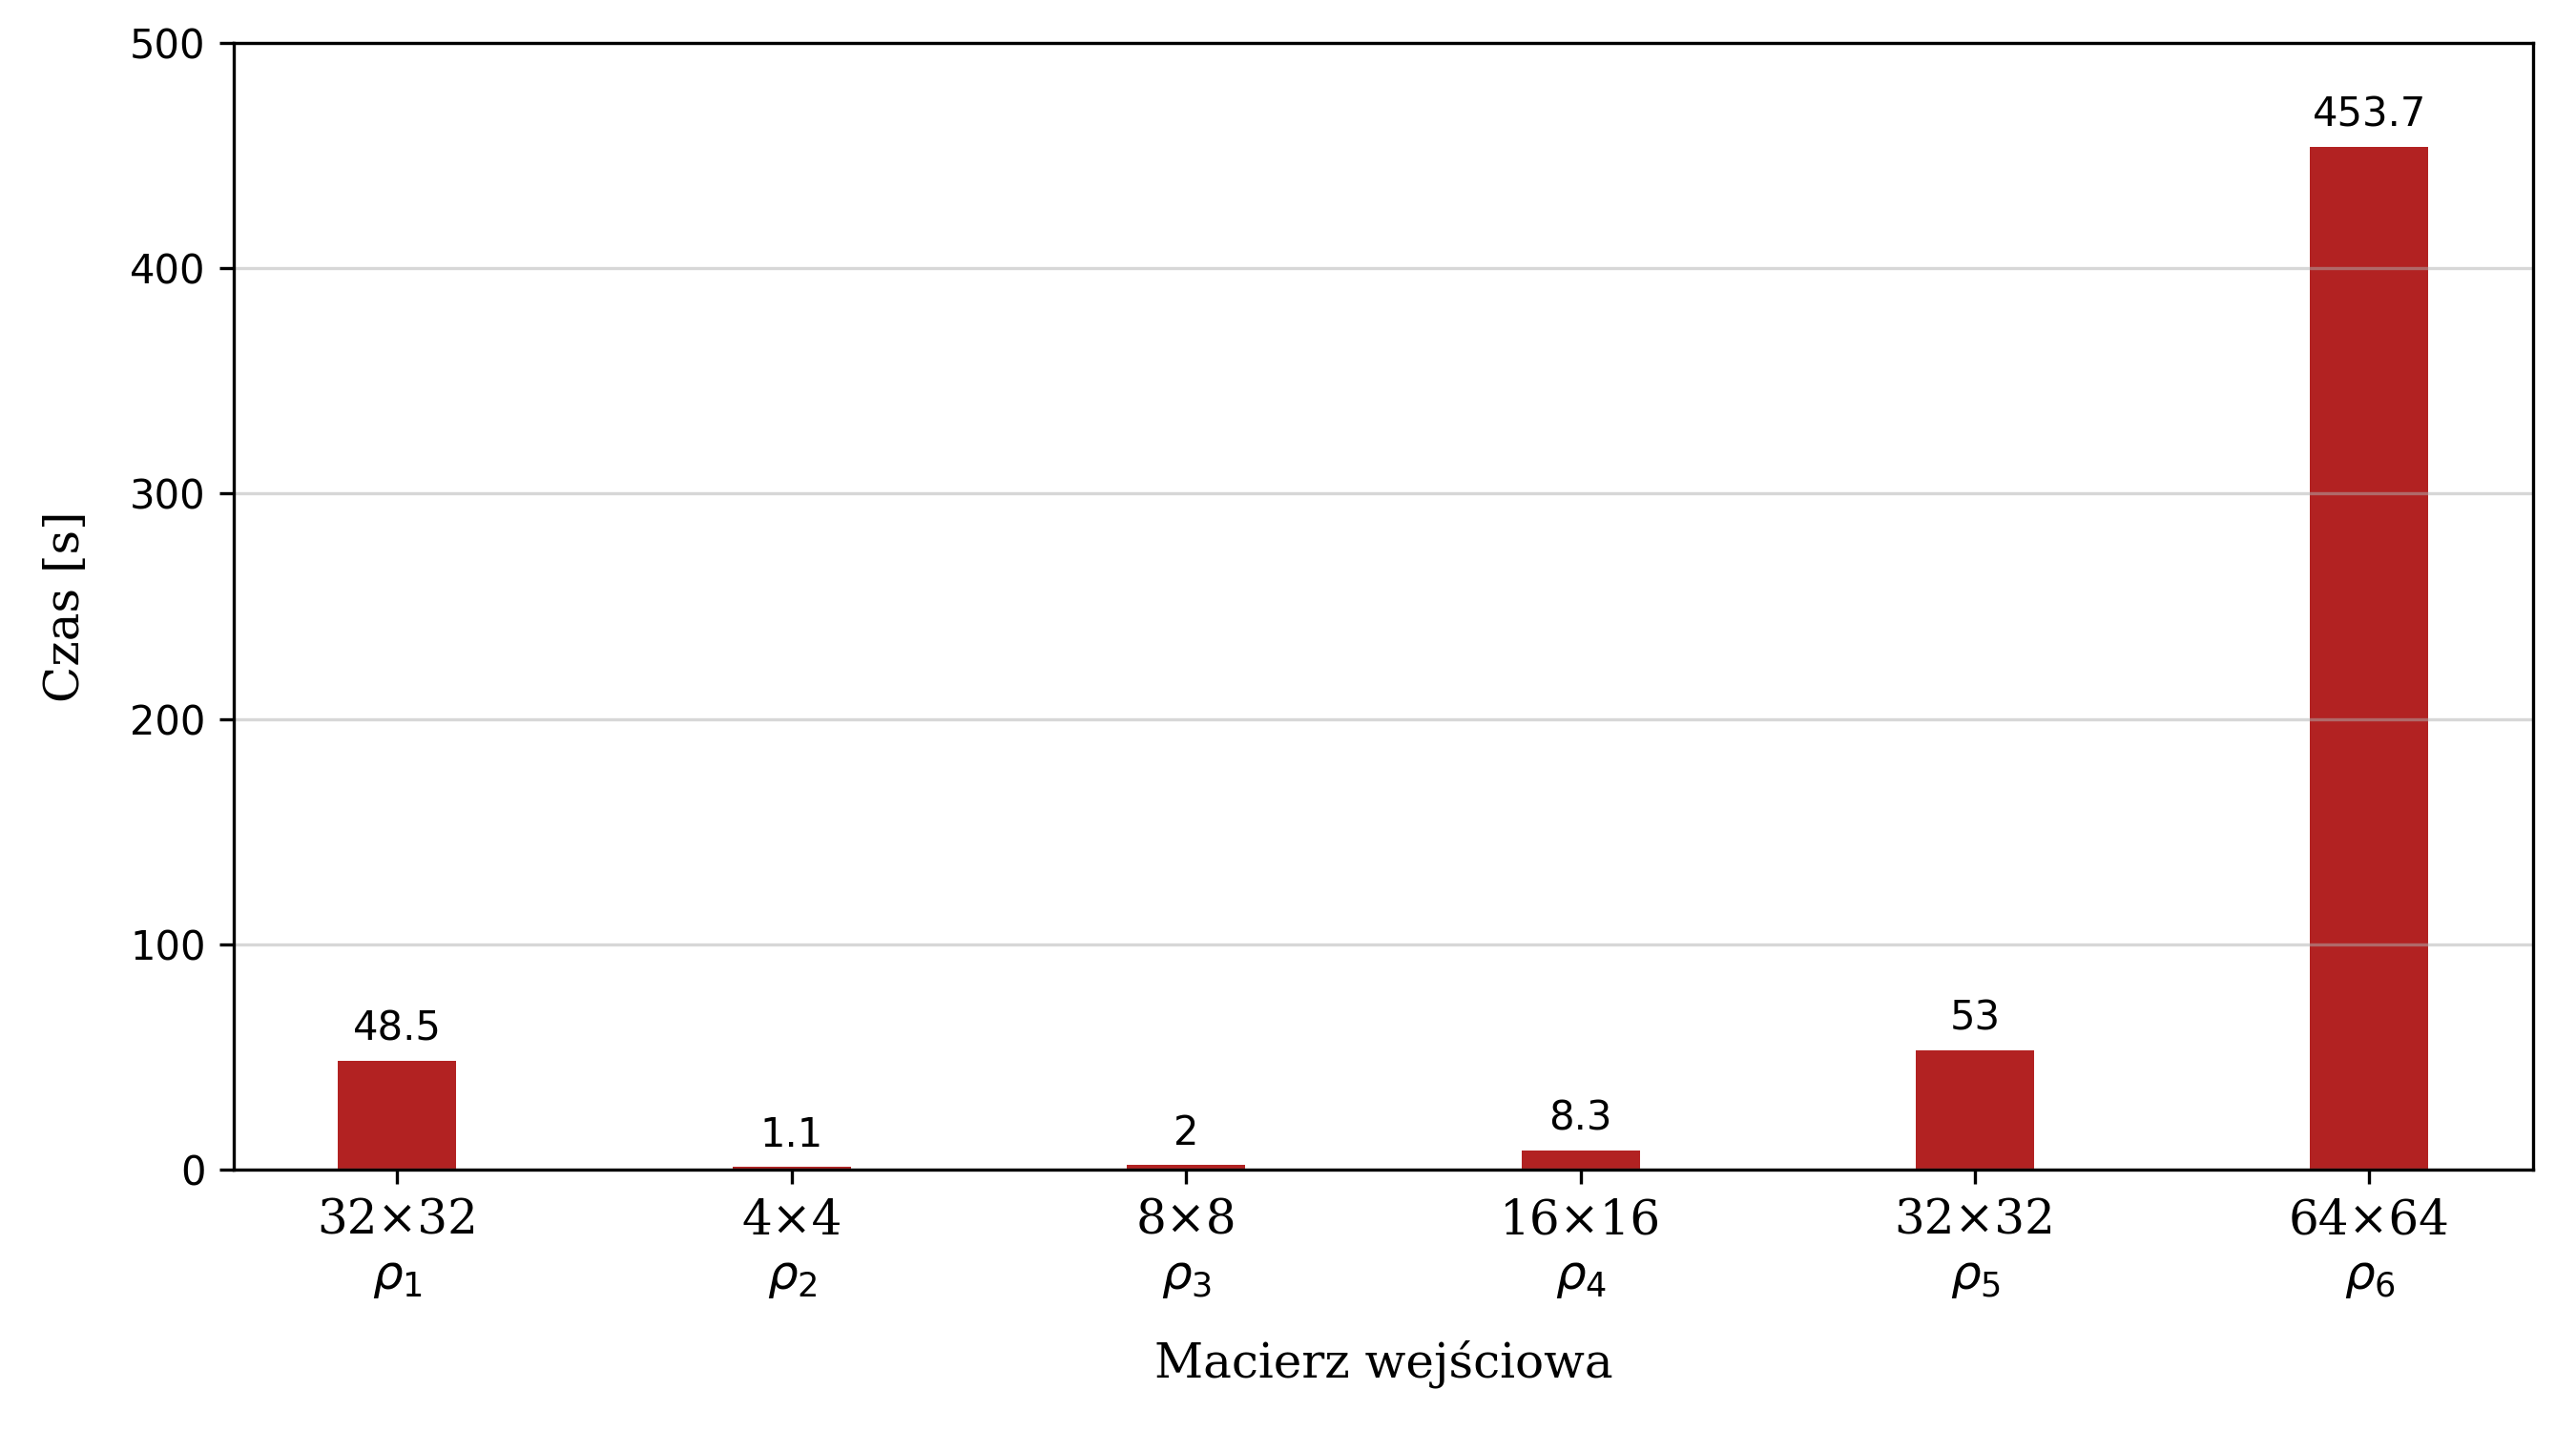
\includegraphics[width=1.0\textwidth]{"resources/rust_performance_tests.png"}
      \caption{Wyniki testów wydajności implementacji w języku Rust dla macierzy $\rho_{1}$ - $\rho
      _{6}$.}
      \label{rust-double-precision}
    \end{figure}

    Na rysunku \ref{rust-double-precision} zaprezentowane zostały wyniki pomiarów czasu
    pracy implementacja w języku Rust. Względem oryginału czas pracy dla małych macierzy
    skrócił się około pięciokrotnie, dotyczy to rozmiarów $4\times4$ i $8\times8$. W przypadku
    macierzy $16\times16$ uzysk jest już tylko dwukrotny, natomiast dla większych
    macierzy uzyskuje ona wyniki gorsze niż oryginał.

    Jest to prawdopodobnie spowodowane tym, że sama implementacja mnożenia macierzowego korzysta
    z ograniczonego zasobu instrukcji SIMD, aby zachować jak najszerszą kompatybilność w
    przeciwieństwie do biblioteki NumPy, która wewnętrznie wykorzystuje bibliotekę OpenBLAS\cite{NumPy_Doc}.

    \FloatBarrier

    \subsubsection{ Rust i Ndaray z OpenBLAS }
    Pomiary czasu pracy implementacji w języku Rust wykorzystującej OpenBLAS do wykonywania
    mnożenia macierzowego były wykonywane w taki sam sposób jak dla implementacji która nie
    korzystała z tej biblioteki.

    \begin{figure}[ht]
      \centering
      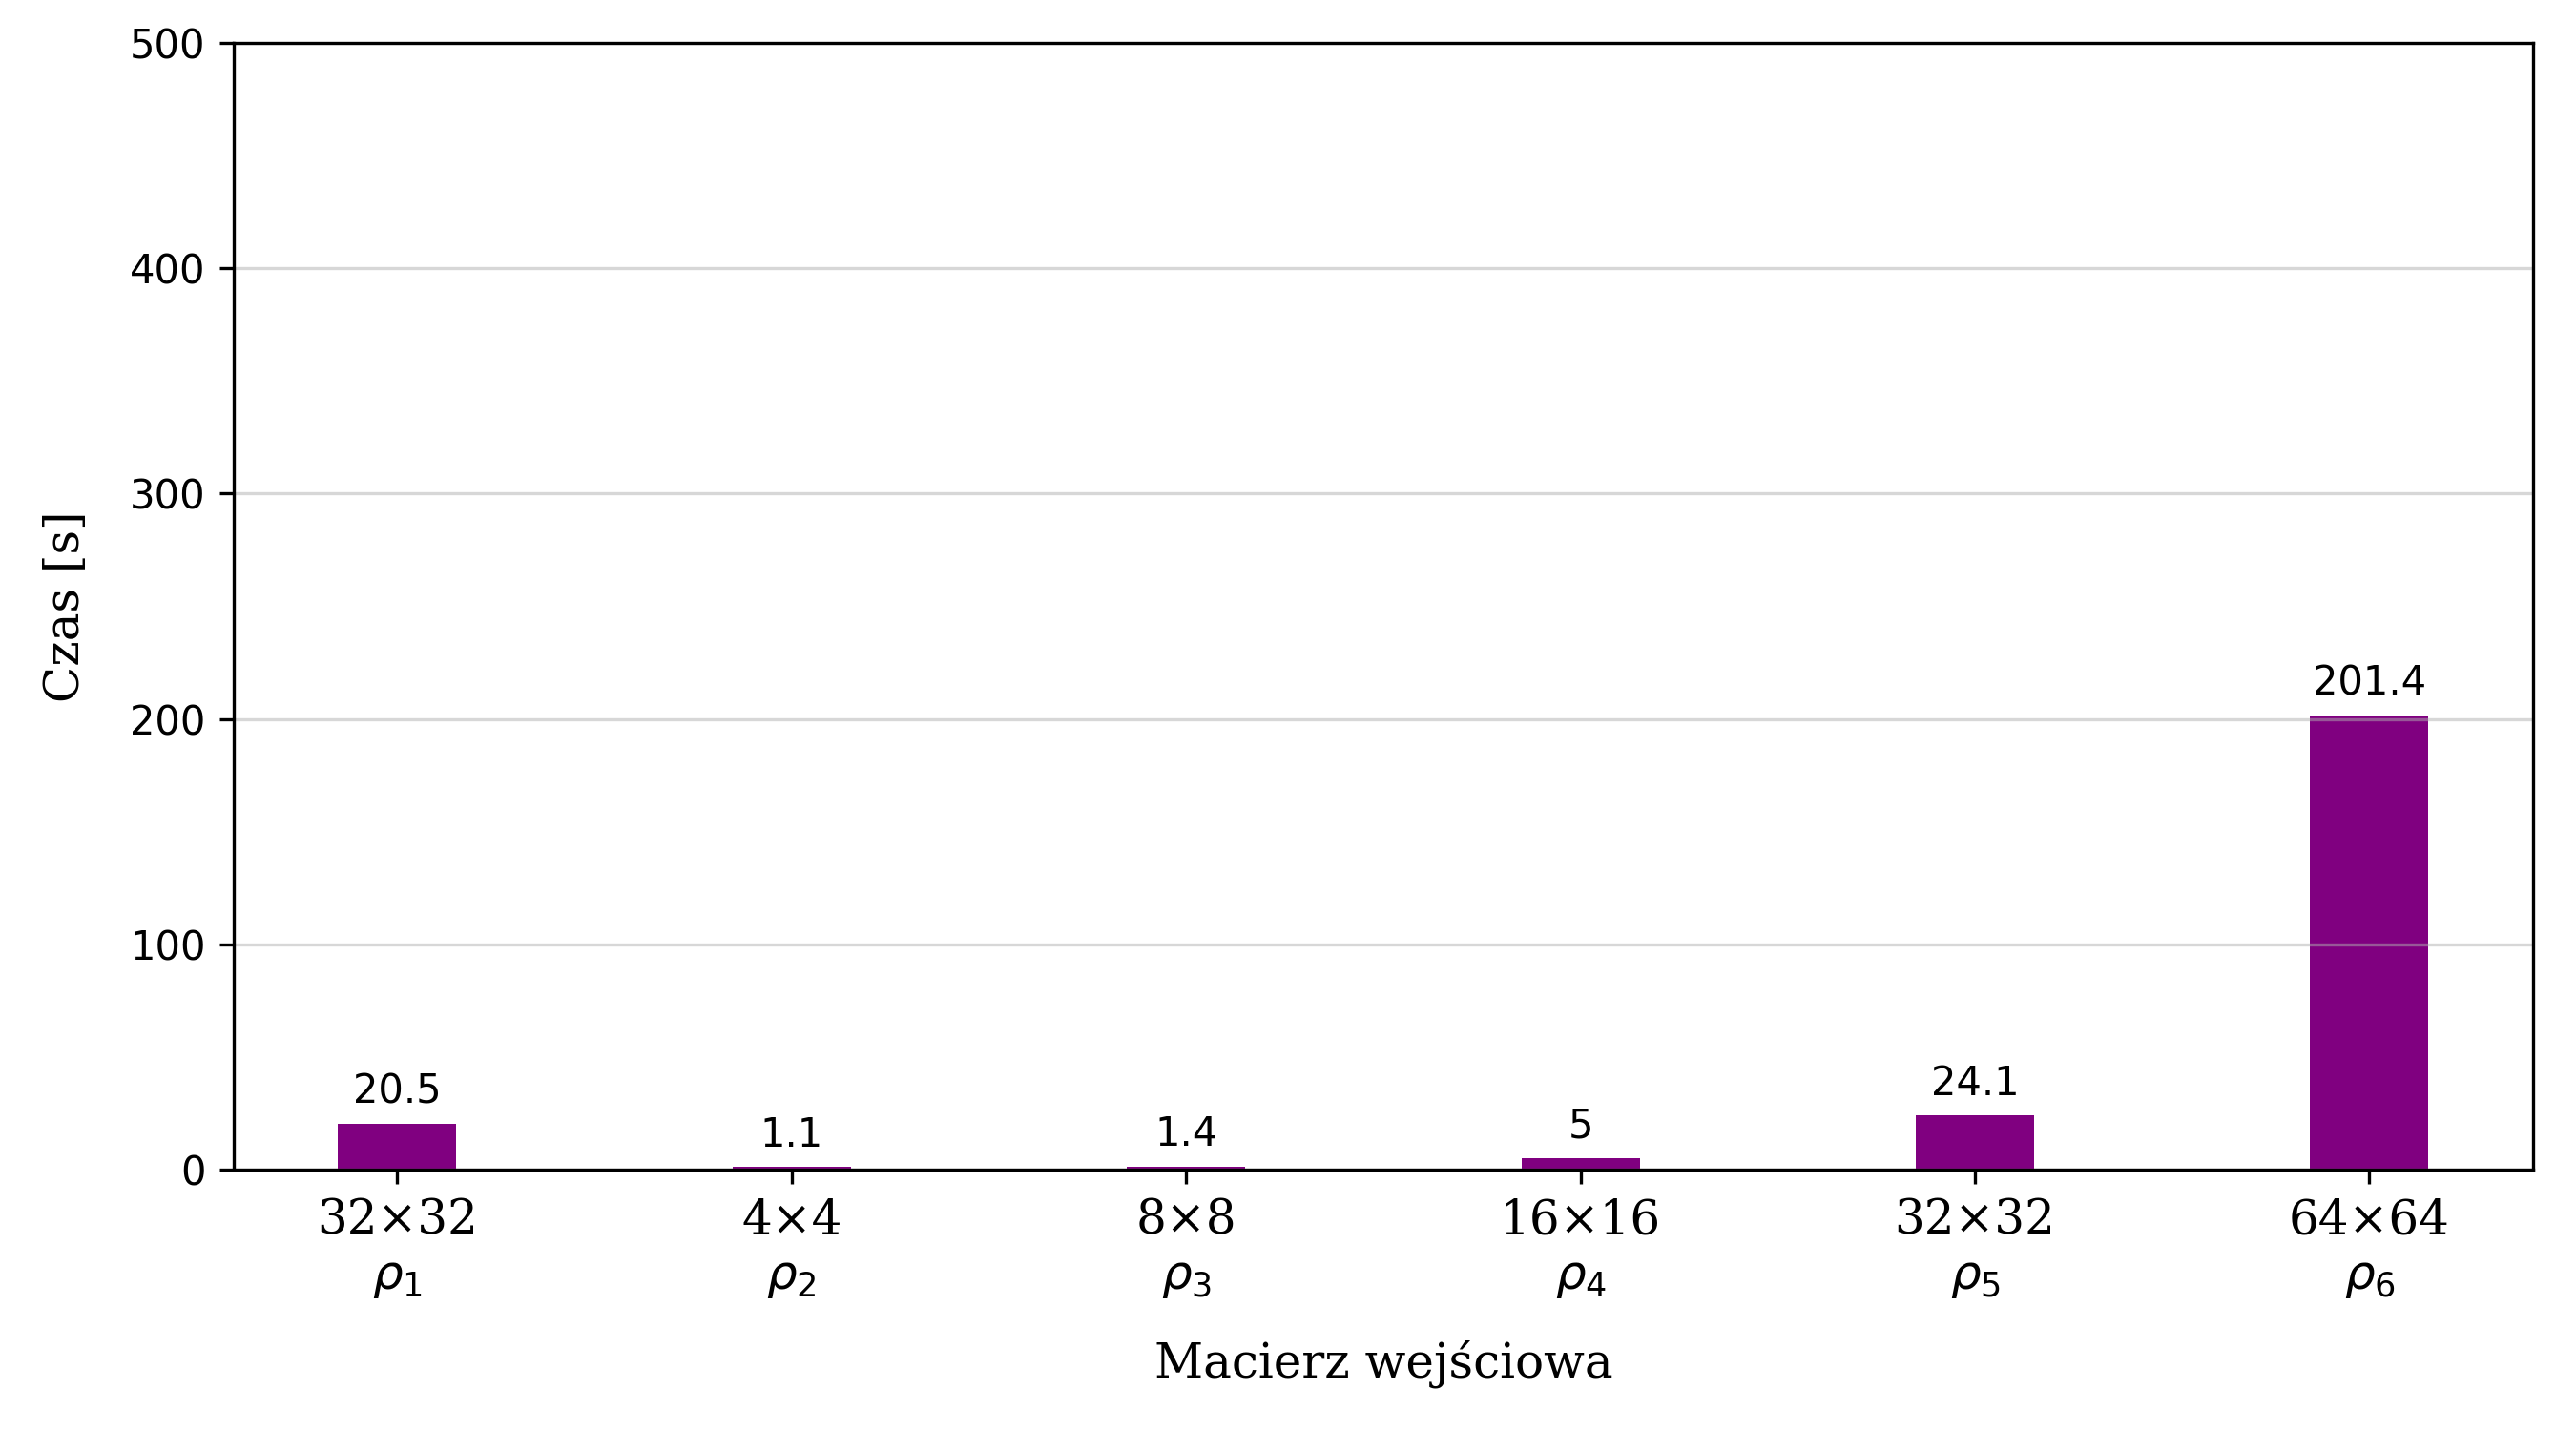
\includegraphics[width=1.0\textwidth]{"resources/rust_blas_perf_tests.png"}
      \caption{Wyniki testów wydajności implementacji w języku Rust z użyciem biblioteki OpenBLAS dla macierzy $\rho
      _{1}$ - $\rho_{6}$.}
      \label{rust-openblas-double-precision}
    \end{figure}

    Wyniki testów przeprowadzanych na implementacji korzystającej z biblioteki OpenBLAS
    poskutkowało znaczącym skróceniem czasu pracy względem oryginału. Wyniki te zaprezentowane
    zostały na rysunku \ref{rust-openblas-double-precision}. Największa różnica
    występuje dla małych macierzy, gdzie podobnie do wariantu nie korzystającego z OpenBLAS,
    przyspieszenie jest około pięciokrotne dla $\rho_{2}$, $\rho_{3}$ i ponad trzykrotne
    dla $\rho_{2}$. Dla macierzy $32\times32$ i $64\times64$ obliczenia zajęły około
    dwukrotnie mniej czasu. Pokazuje to jak znaczący wzrost wydajności można uzyskać przy
    pomocy wyspecjalizowanego kodu w języku Asemblera, który został wykorzystany w
    bibliotece OpenBLAS do stworzenia wyspecjalizowanych implementacji mnożenia
    macierzowego.

    \FloatBarrier

    \subsection{Pomiary z pojedynczą precyzją}
    Wszystkie testy wydajności z dla obliczeń wykorzystujących liczby zmiennoprzecinkowe
    pojedynczej precyzji były przeprowadzane w taki sam sposób jak odpowiadające testy z
    podwójną precyzją.

    \subsubsection{ Python i NumPy }
    \begin{figure}[ht]
      \centering
      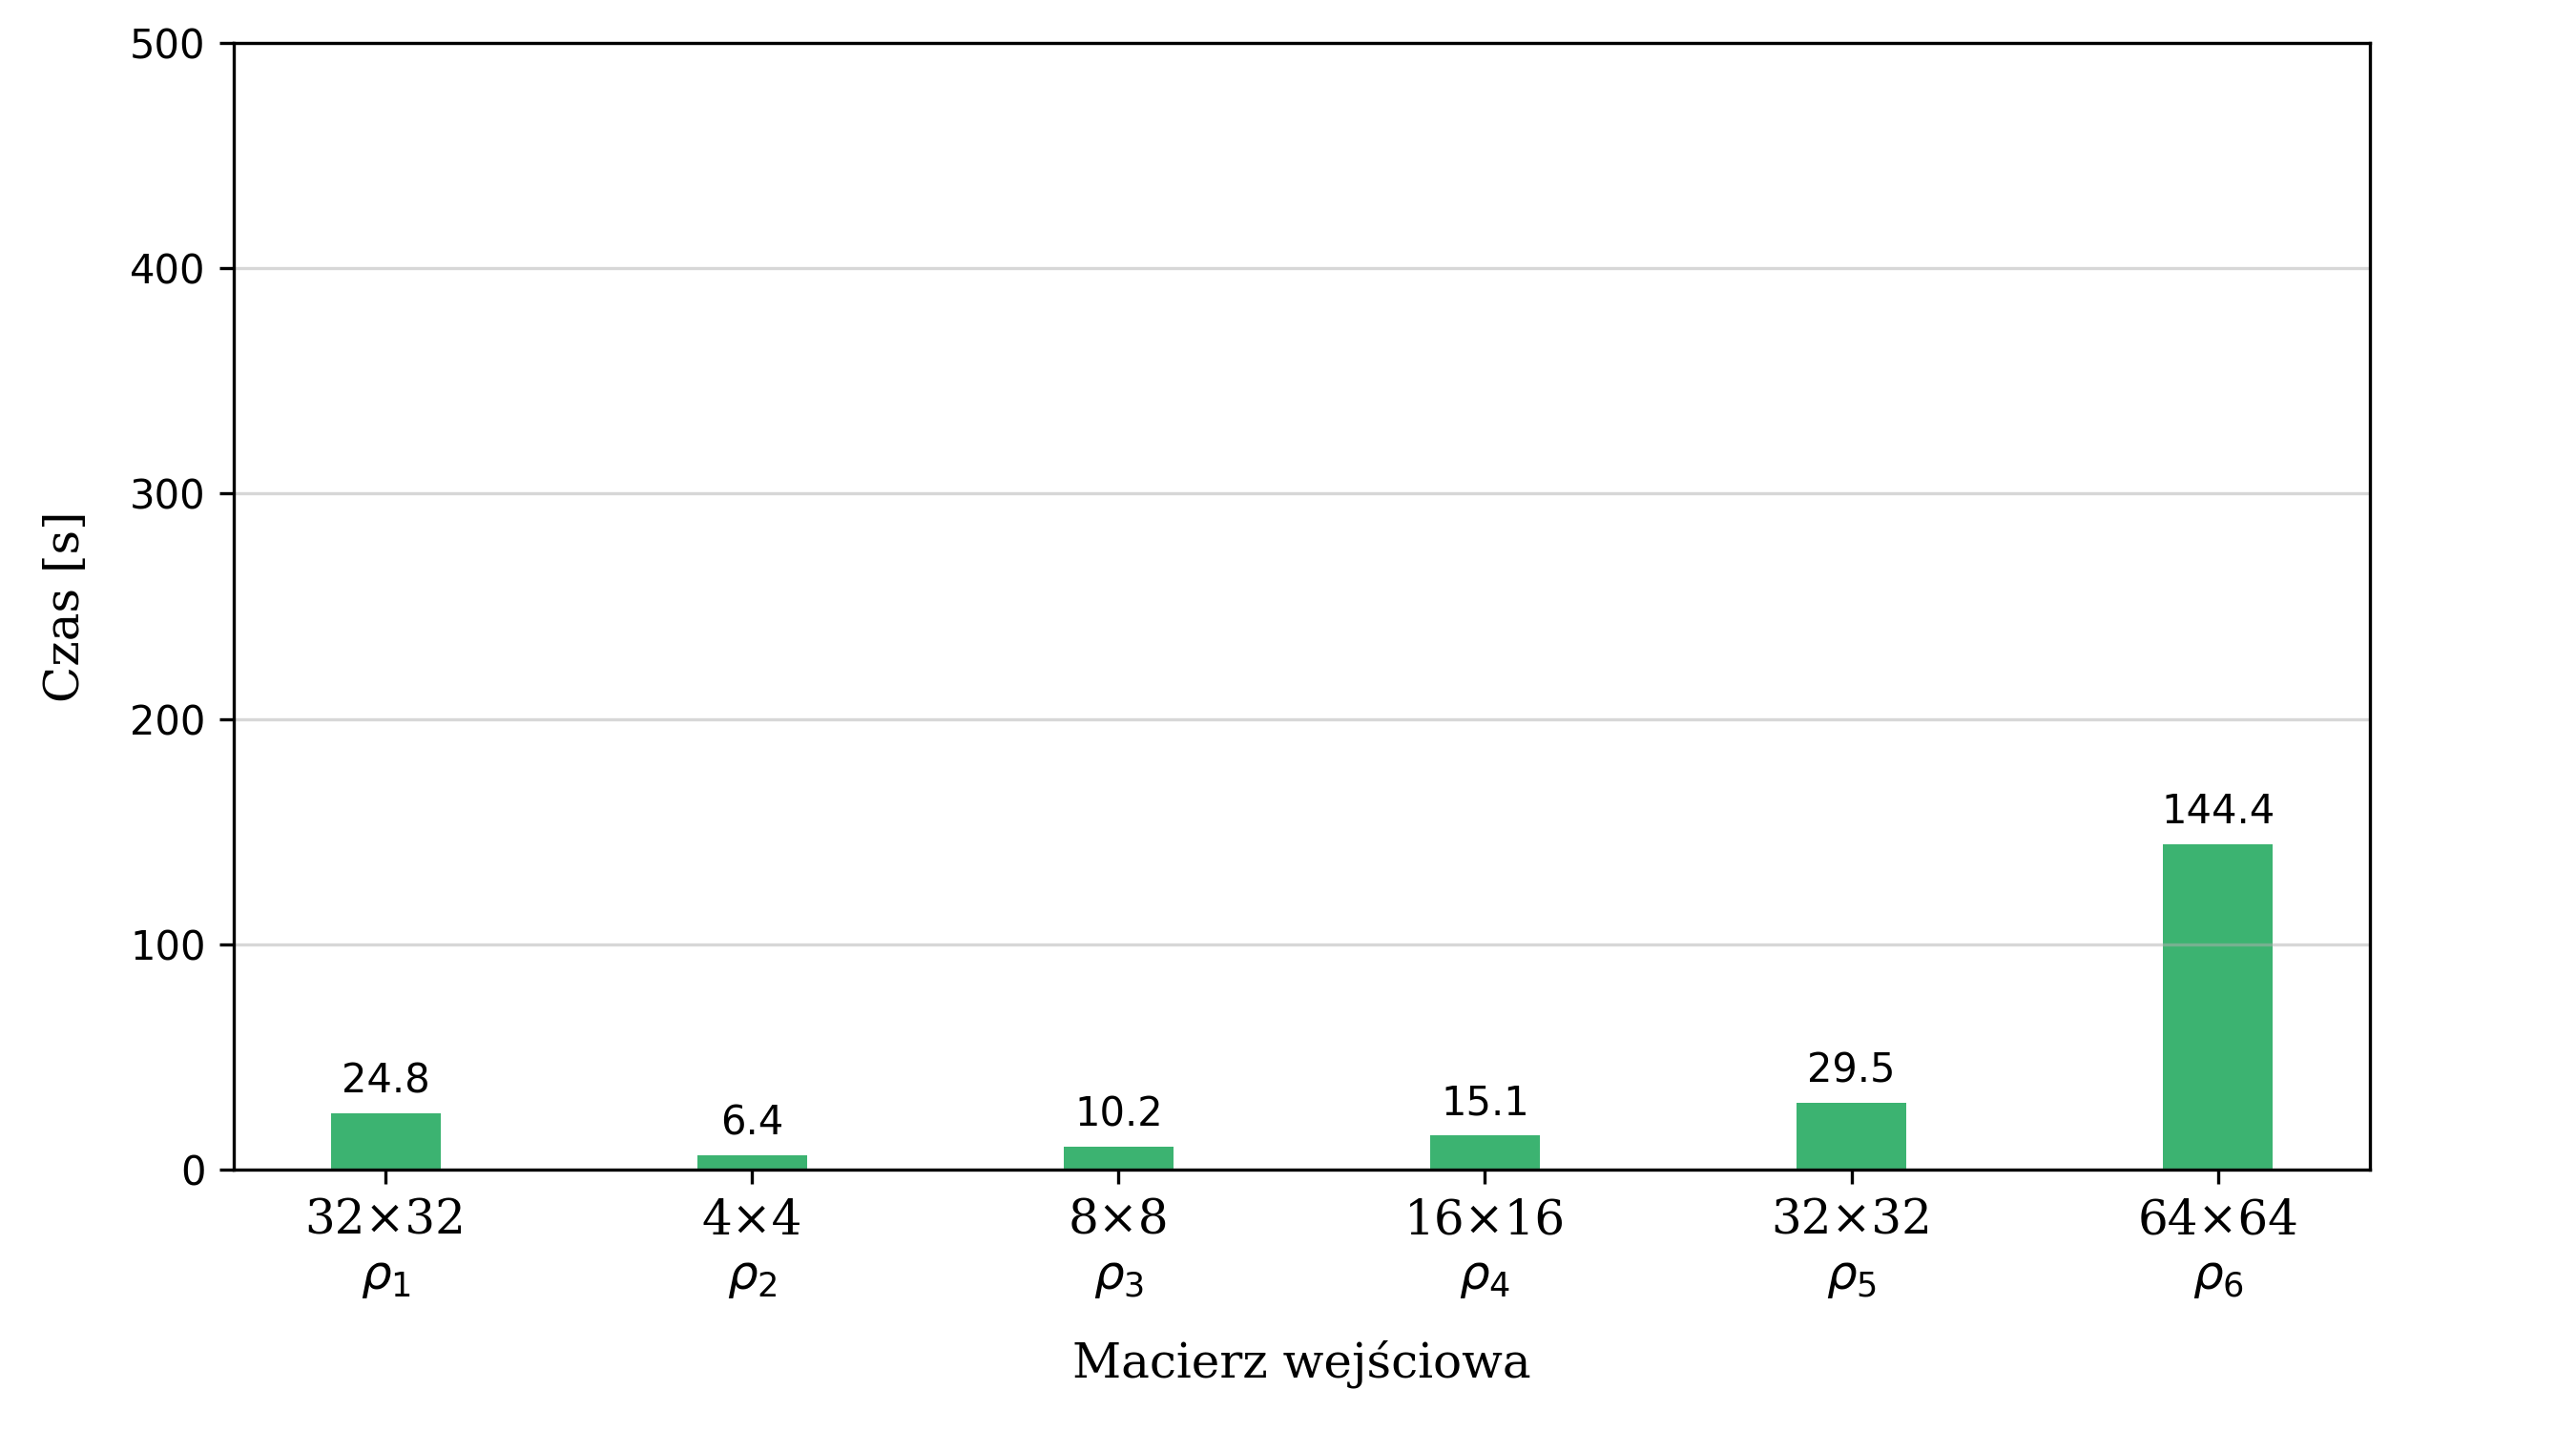
\includegraphics
      [width=1.0\textwidth]{"resources/python_and_numpy_single_tests.png"}
      \caption{Wyniki testów wydajności implementacji w języku Python z użyciem biblioteki NumPy dla macierzy $\rho
      _{1}$ - $\rho_{6}$ i obliczeniami pojedynczej precyzji.}
      \label{sp-numpy-perf}
    \end{figure}

    Na wykresie \ref{sp-numpy-perf} przedstawiłem wyniki wydajności dla implementacji
    napisanej w języku Python wykorzystującej bibliotekę NumPy do przeprowadzania
    obliczeń na macierzach liczb zespolonych pojedynczej precyzji. W przypadku mniejszych
    macierzy ($4\times4$, $8\times8$, $16\times16$) różnice w czasie pracy, względem
    wariantu opartego na liczbach podwójnej precyzji, są minimalne. Dzieje się tak
    prawdopodobnie dlatego, że macierze te są na tyle niewielkie (do 4KB) że mieszczą się
    w pamięci cache L1 procesora\footnote{Wykorzystywany tutaj Ryzen 9 7950X posiada
    $32\times16$KB cache L1}, więc wymnażanie ich jest procesem bardzo szybkim. W
    momencie kiedy docieramy do macierzy $32\times32$ wzrost wydajności staje się
    zauważalny, co również można wytłumaczyć odwołując się do pojemności pamięci cache procesora.
    Macierze podwójnej precyzji zajmują dokładnie 16KB ($32\times 32\times2\times 8$), natomiast
    dostęp do tej pamięci nie jest ekskluzywny dla jednego procesu, nie może on więc
    korzystać z całych 16KB. W efekcie część danych przebywa poza pamięcią cache.
    Natomiast macierze wykorzystujące liczby pojedynczej precyzji zajmują tylko 8KB. Można
    się więc spodziewać że większość czasu spędzają one w pamięciach L1 i L2, co pozwala
    przyspieszyć obliczenia. Dodatkowo mniejszy rozmiar liczb pojedynczej precyzji pozwala
    dwukrotnie zwiększyć przepustowość instrukcji SIMD, co prawdopodobnie odgrywa
    również bardzo istotną rolę, szczególnie w przypadku macierzy $64\times64$, dla
    których obliczenia przyspieszają znacznie bardziej niż w przypadku mniejszych
    macierzy.

    \FloatBarrier

    \subsubsection{ Python i NumPy z AOT }
    \begin{figure}[ht]
      \centering
      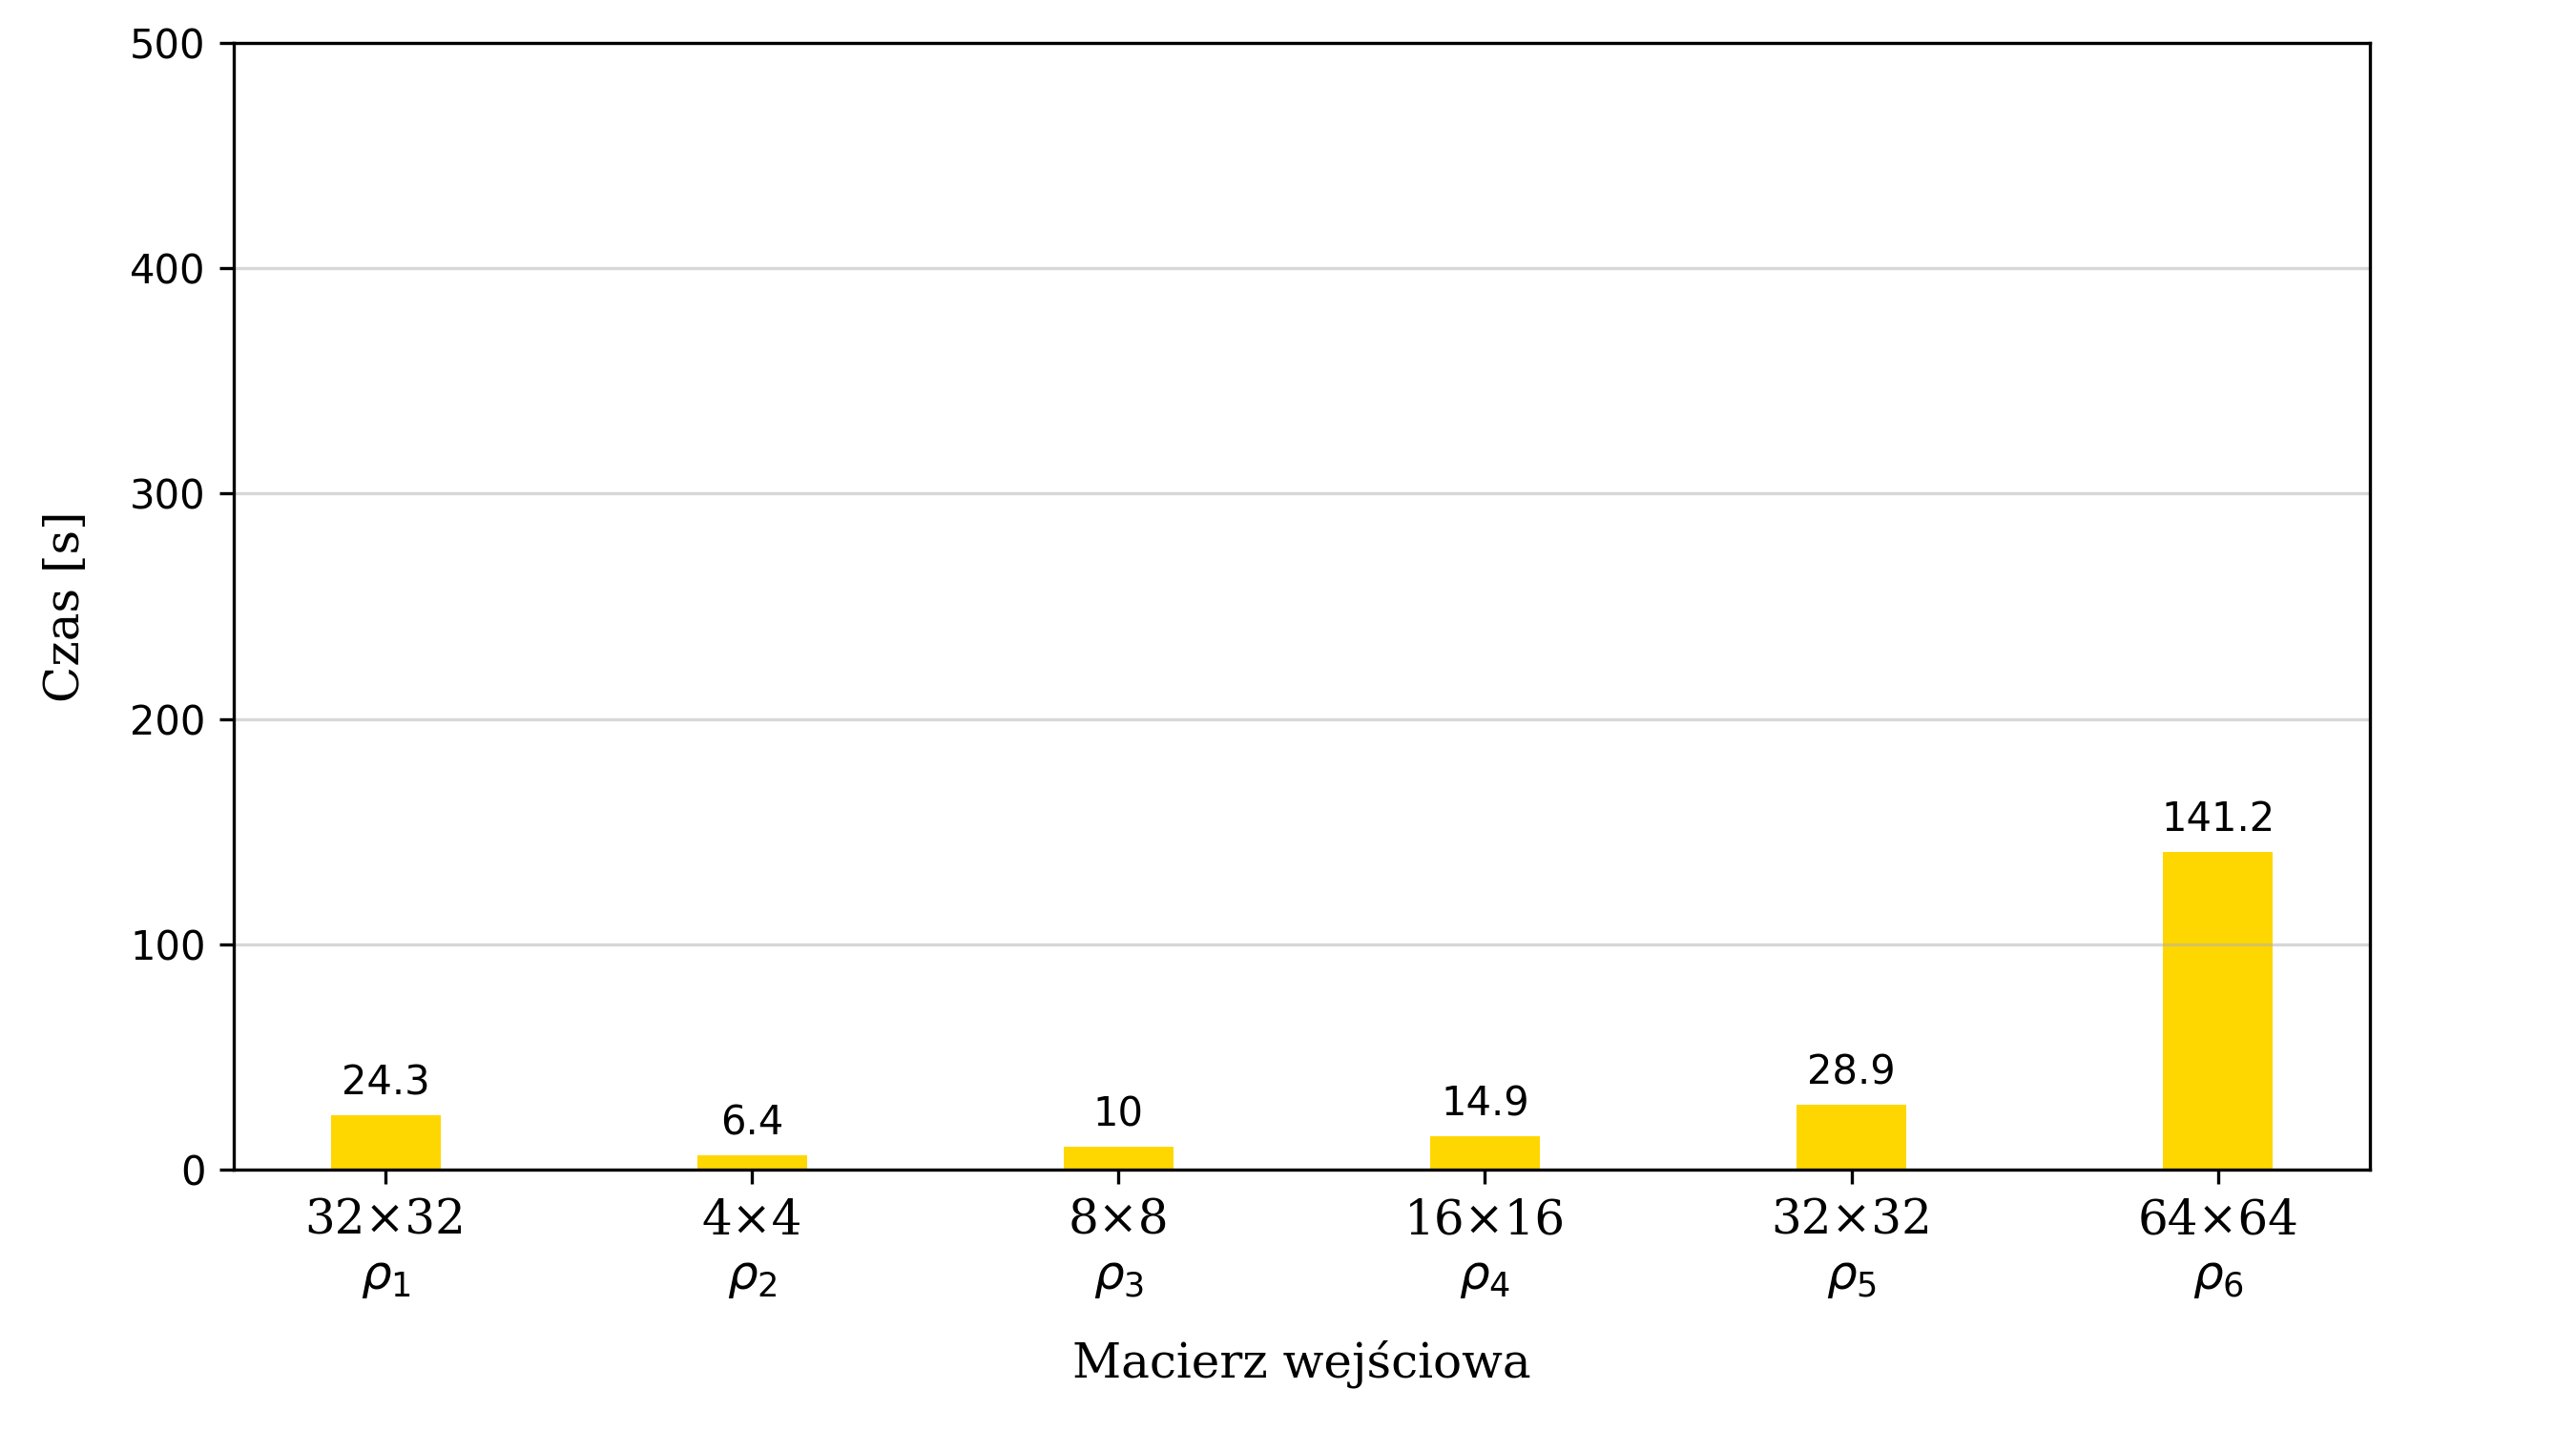
\includegraphics
      [width=1.0\textwidth]{"resources/python_and_numpy_and_aot_single_tests.png"}
      \caption{Wyniki testów wydajności implementacji w języku Python z użyciem biblioteki NumPy i pakietu Cython do kompilacji AOT dla macierzy $\rho
      _{1}$ - $\rho_{6}$ i obliczeniami pojedynczej precyzji.}
      \label{python-numpy-cython-single-precision}
    \end{figure}

    Wyniki dla wariantu pre-kompilowanego przy pomocy biblioteki Cython nie różnią się
    znacząco od wariantu nie pre-kompilowanego, podobnie jak w przypadku obliczeń podwójnej
    precyzji, zostały one zaprezentowane na rysunku
    \ref{python-numpy-cython-single-precision}. Podobnie jak w przypadku wyników dla obliczeń
    podwójnej precyzji, pre-kompilacja nie przynosi istotnych zysków wydajnościowych.

    \FloatBarrier

    \subsubsection{ Python i NumPy z JIT }
    \begin{figure}[ht]
      \centering
      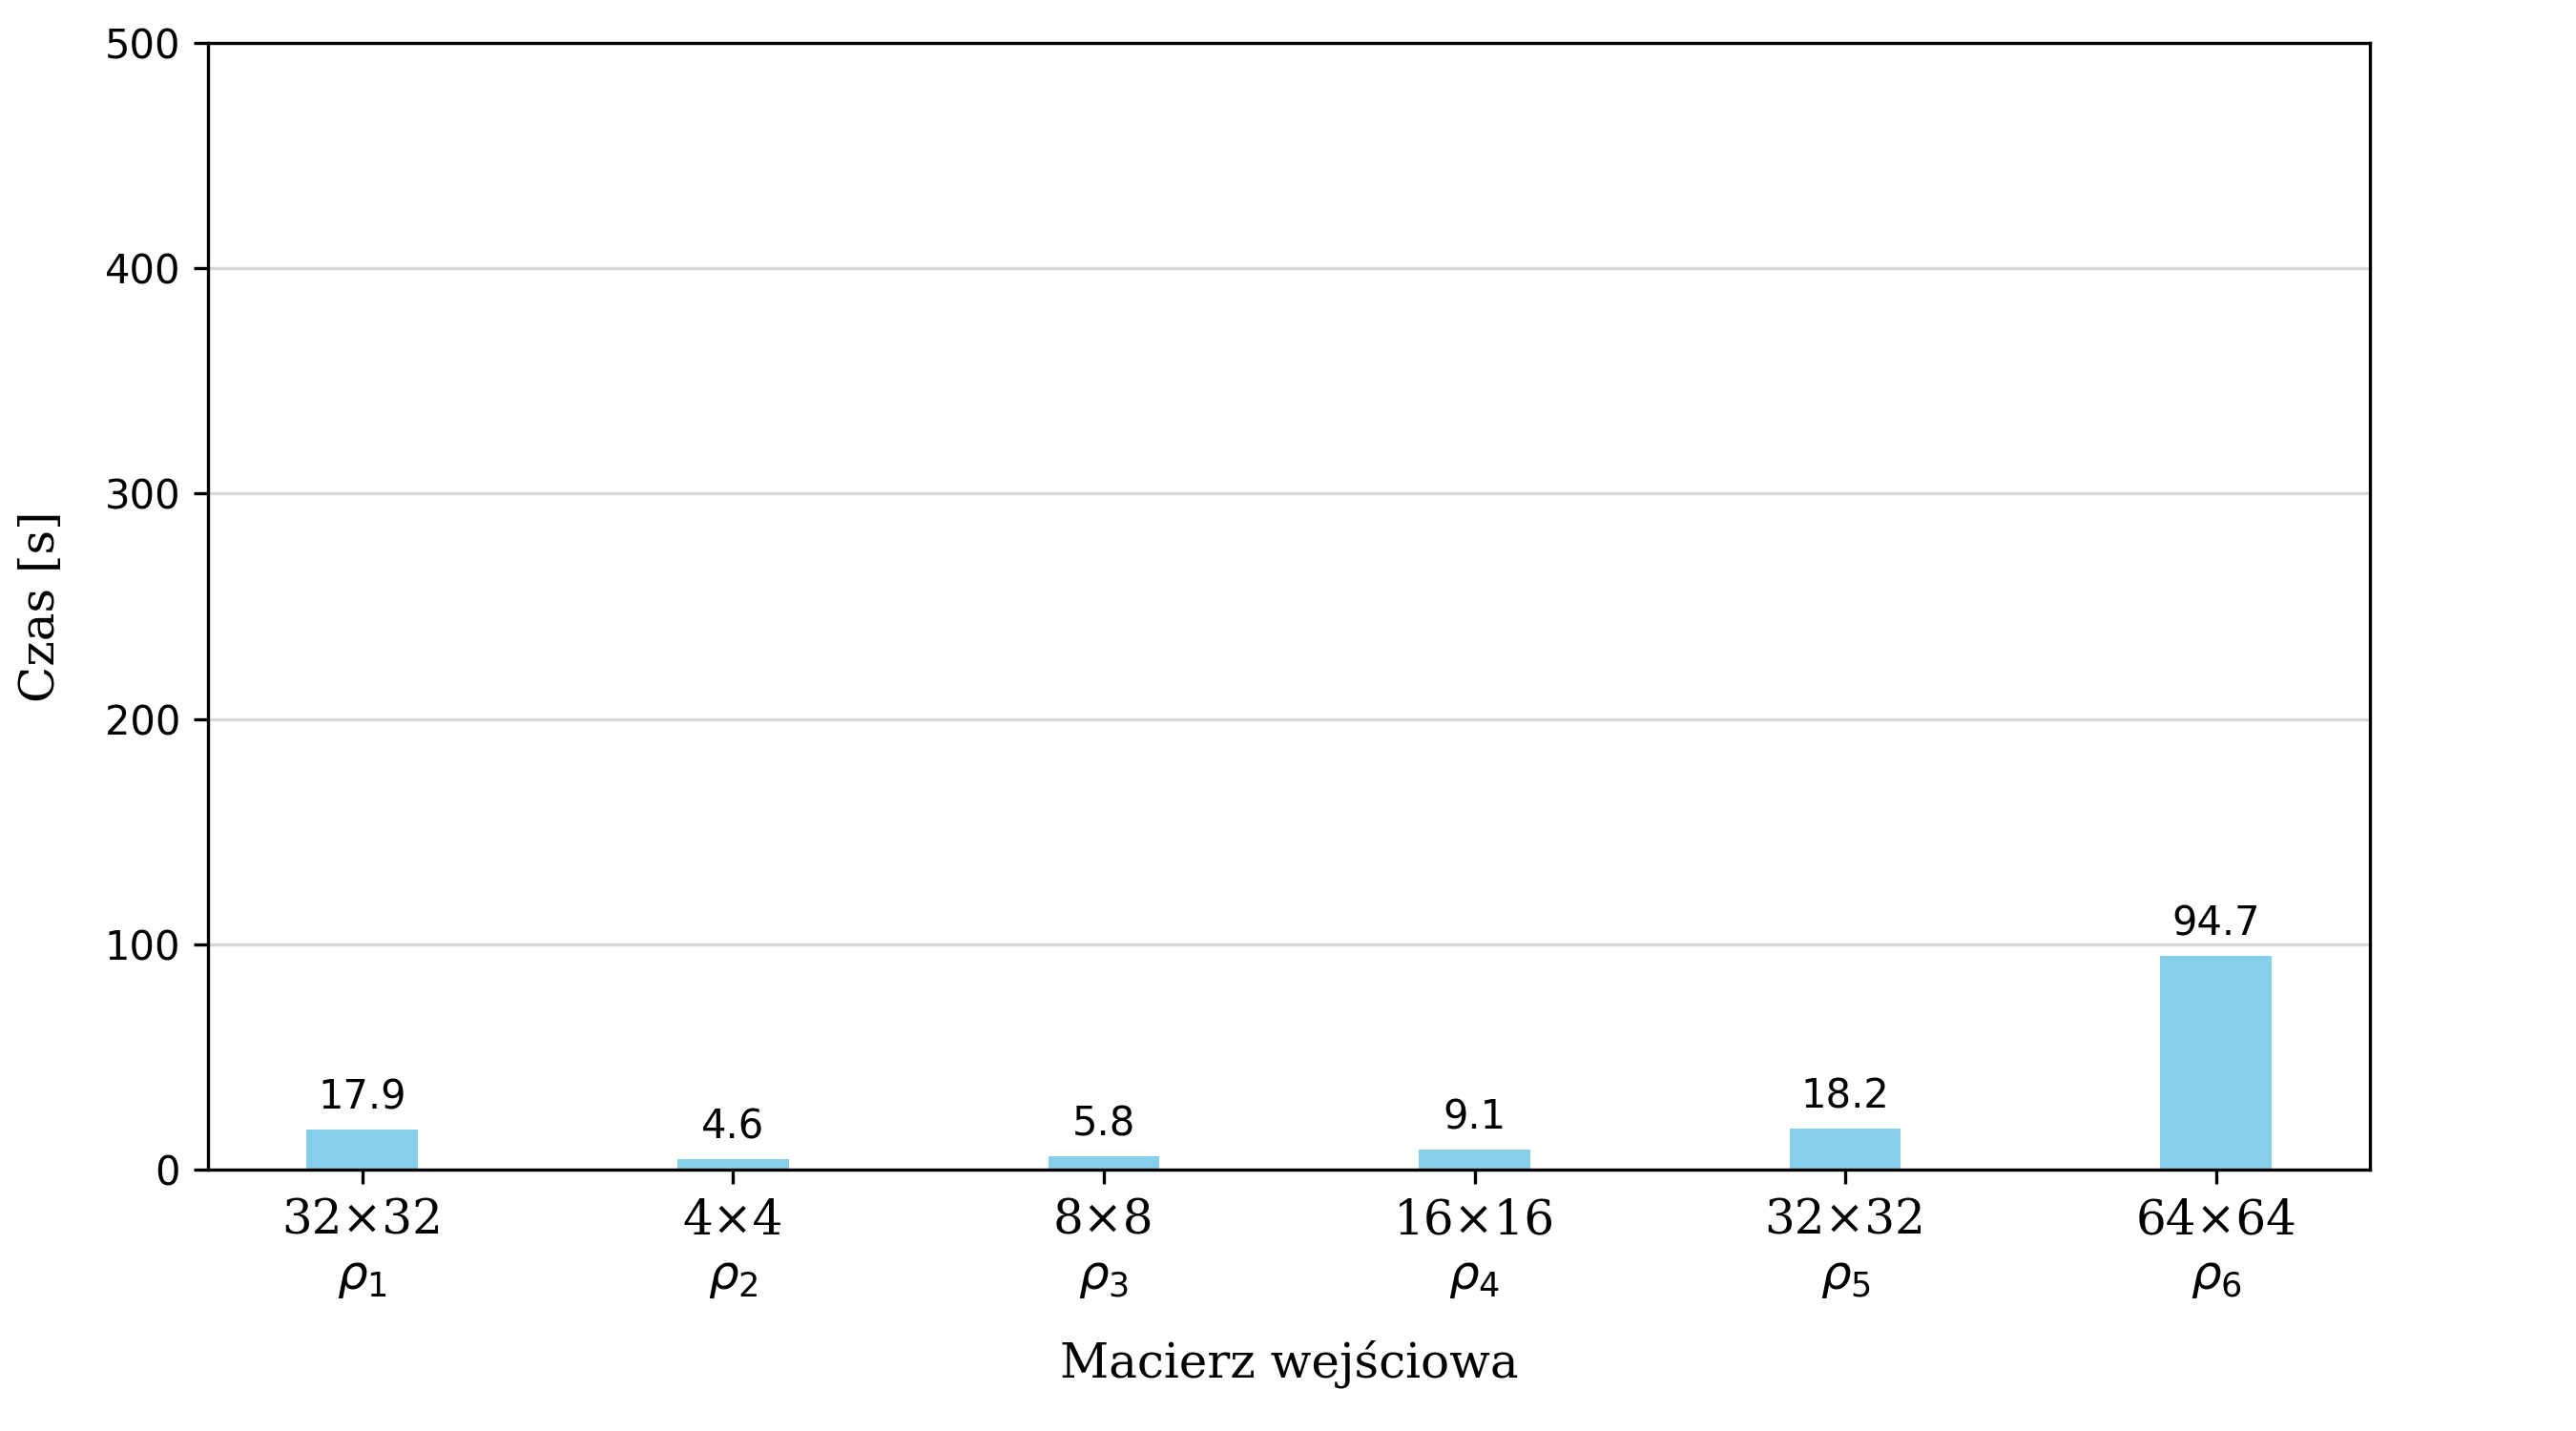
\includegraphics
      [width=1.0\textwidth]{"resources/python_and_numpy_and_jit_single_tests.png"}
      \caption{Wyniki testów wydajności implementacji w języku Python z użyciem biblioteki NumPy i pakietu Numba do kompilacji JIT dla macierzy $\rho
      _{1}$ - $\rho_{6}$ i obliczeniami pojedynczej precyzji.}
      \label{sp-numpy-jit-perf}
    \end{figure}

    W przypadku wariantu wykorzystującego kompilację JIT, zysk czasowy wynikający z redukcji
    precyzji obliczeń jest minimalny lub wręcz nie występuje. Wyjątkiem są tutaj wyniki
    dla macierzy $\rho_{1}$ w przypadku której czas pracy skrócił się o $4.7s$ (
    $\approx 21\%$).

    \FloatBarrier

    \subsubsection{ Rust i Ndaray}
    \begin{figure}[ht]
      \centering
      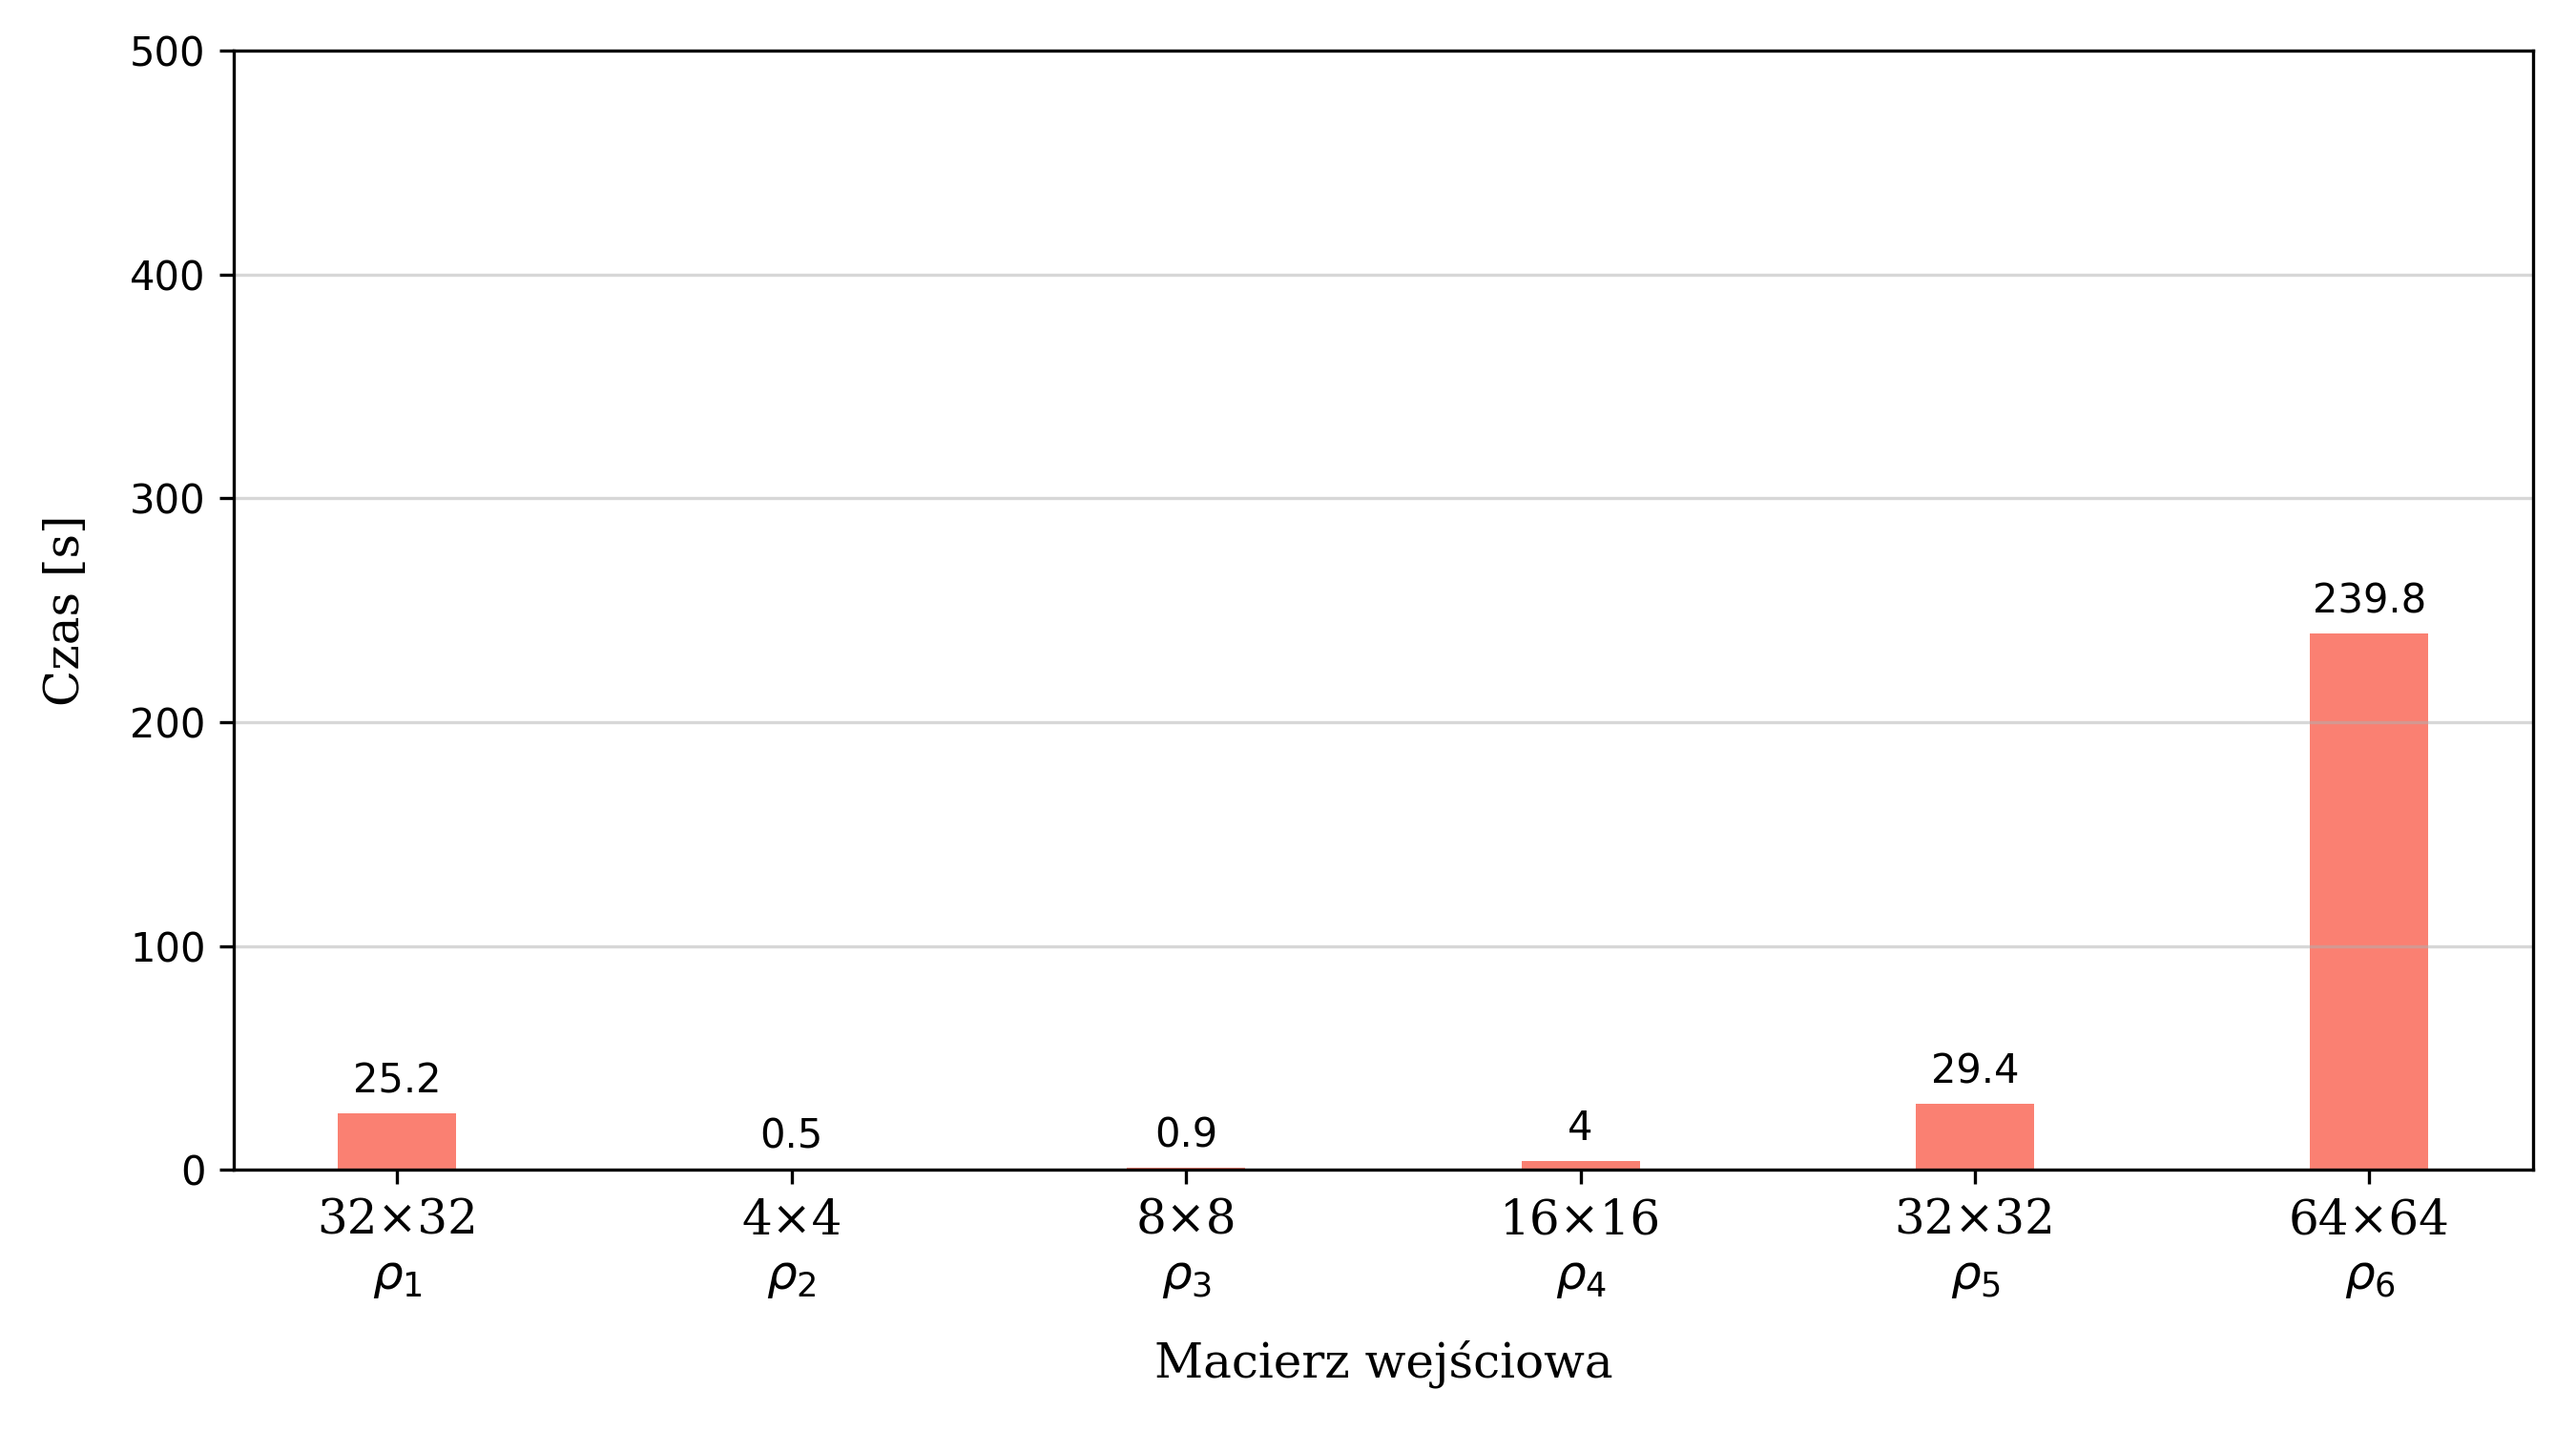
\includegraphics[width=1.0\textwidth]{"resources/rust_single_tests.png"}
      \caption{Wyniki testów wydajności implementacji w języku Rust z użyciem biblioteki Ndarray dla macierzy $\rho
      _{1}$ - $\rho_{6}$ i obliczeniami pojedynczej precyzji.}
      \label{sp-rust-perf}
    \end{figure}

    Implementacja w języku Rust wykorzystująca bibliotekę Ndarray prezentuje znaczną poprawę
    wydajności dla wszystkich wymiarów macierzy. Podczas obliczeń na małych macierzach, do
    $16\times16$ włącznie, uzyskuje ona najlepsze wyniki w zestawieniu, natomiast dla większych
    macierzy poprawa występuje, ale ciągle implementacja w języku Python z JIT daje
    lepsze efekty.

    \FloatBarrier

    \subsubsection{ Rust i Ndaray z OpenBLAS }
    \begin{figure}[ht]
      \centering
      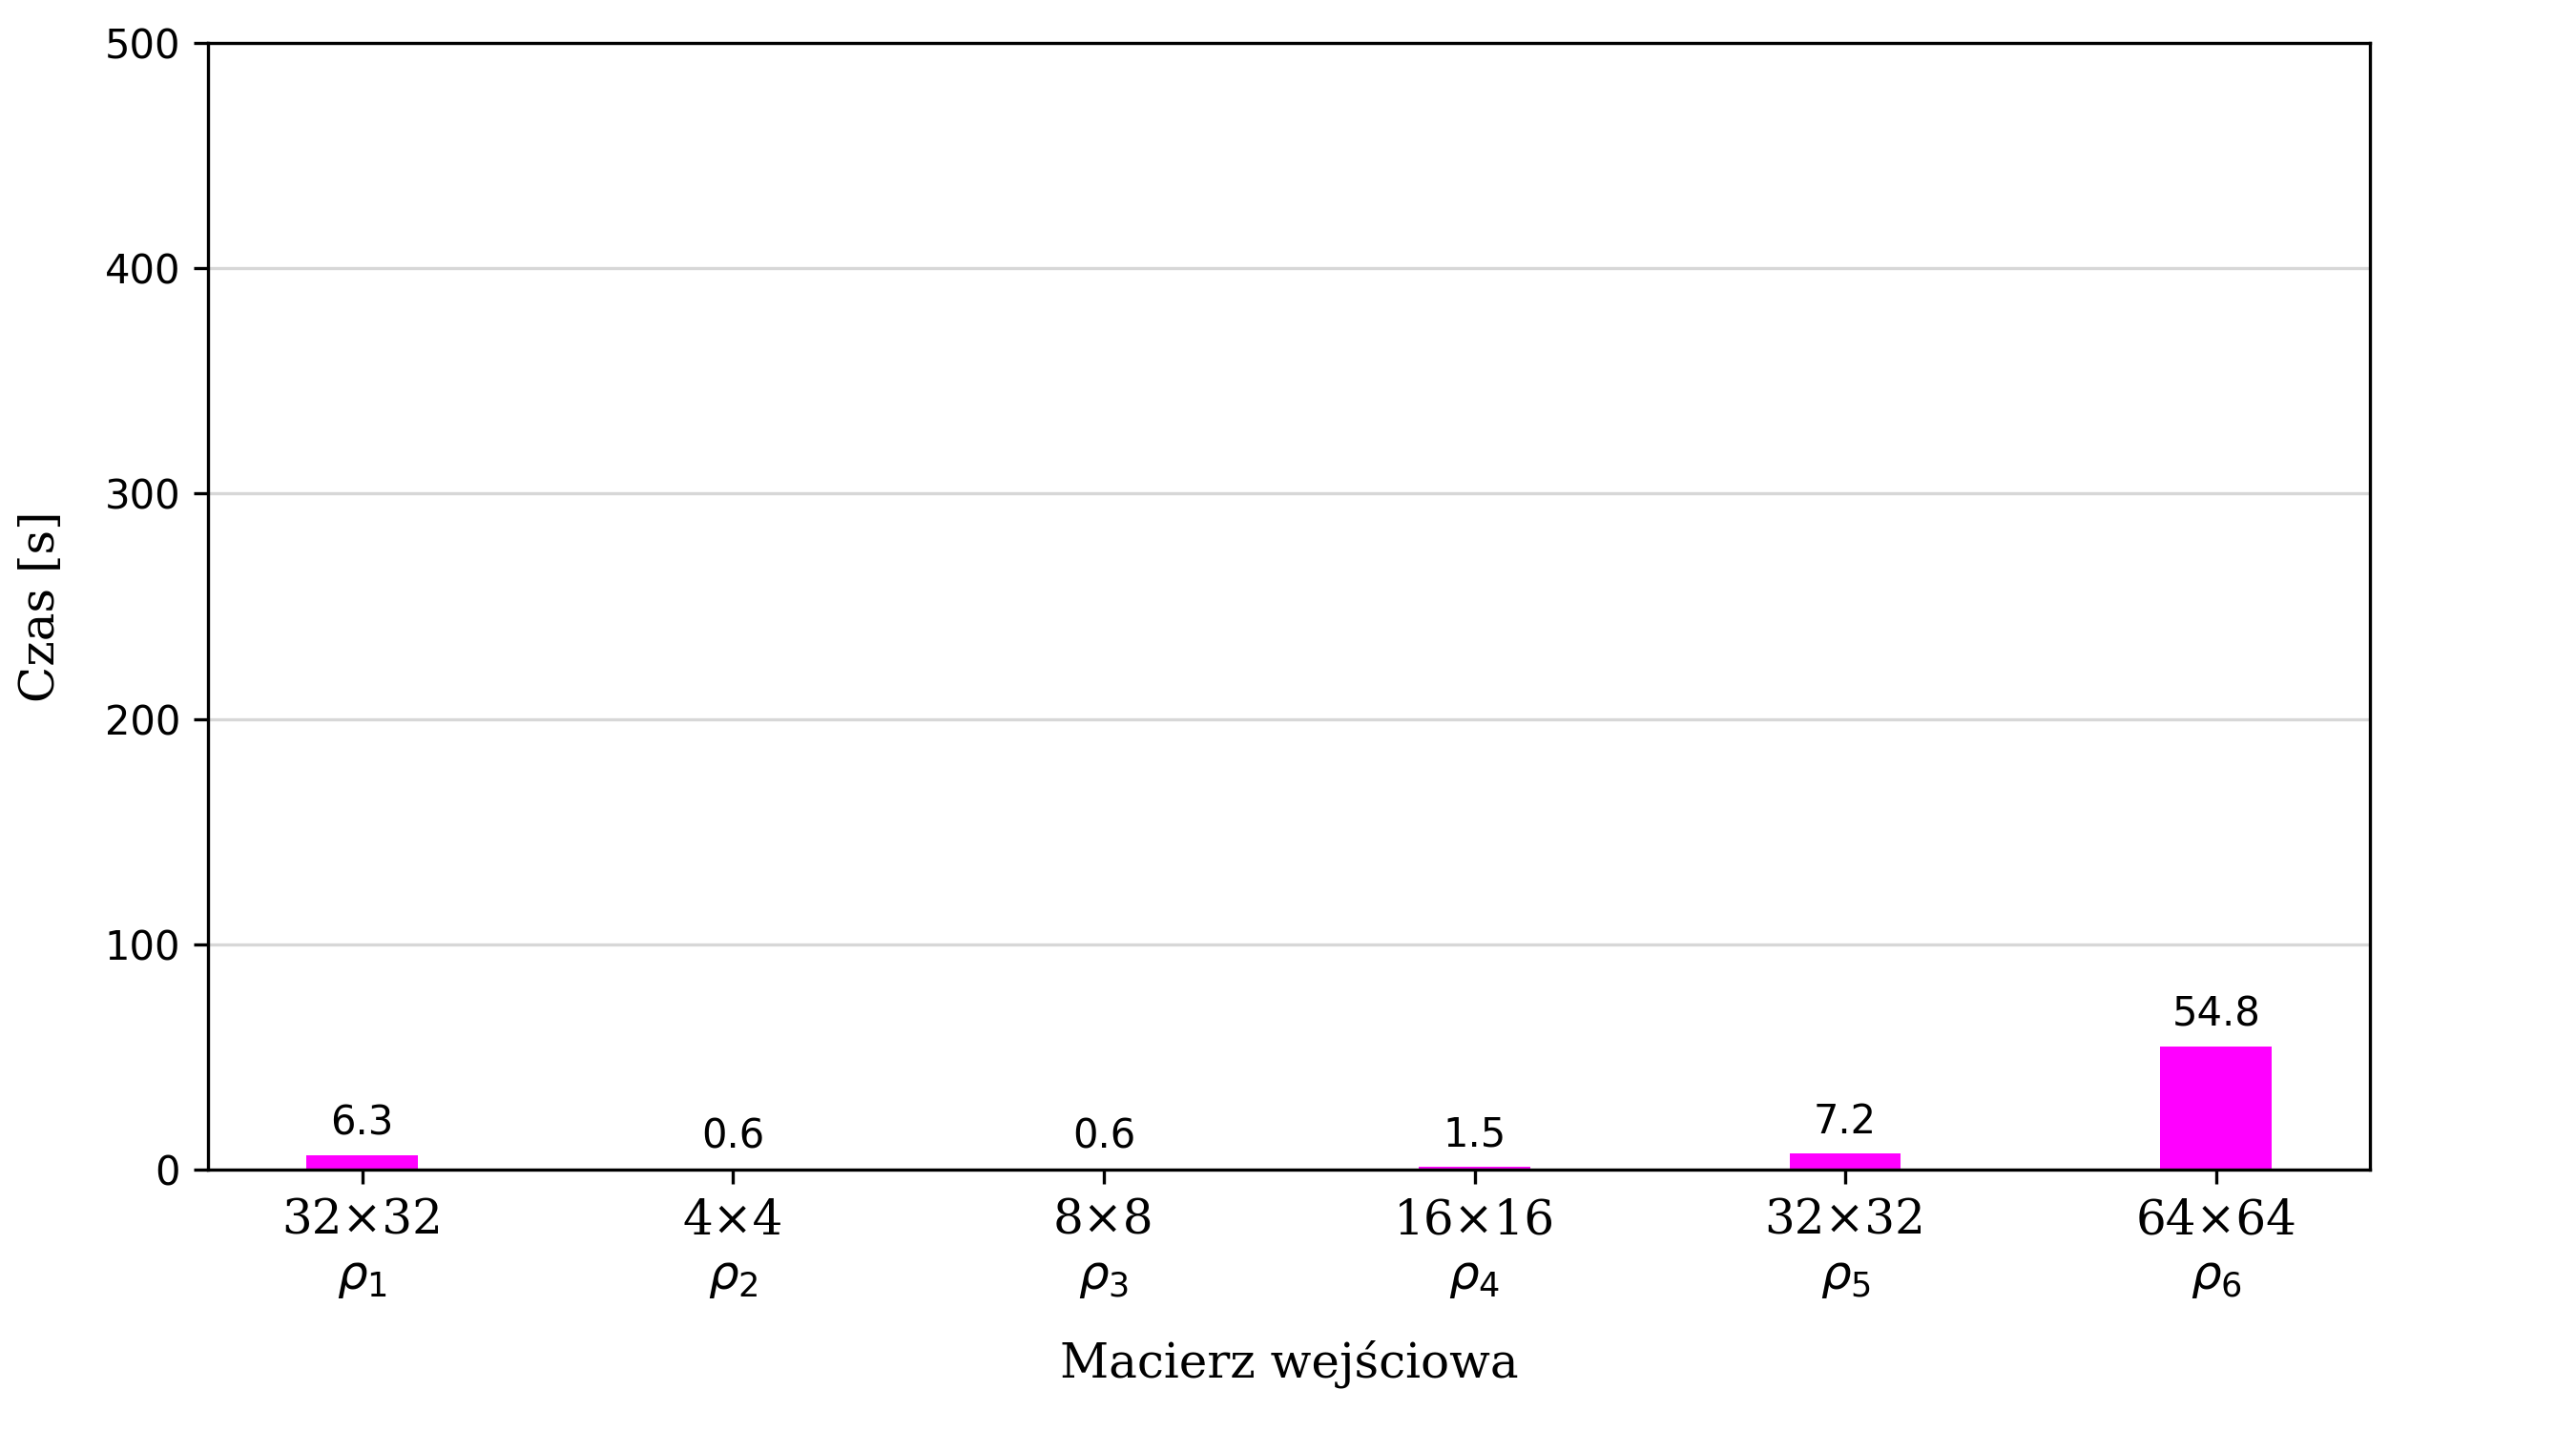
\includegraphics[width=1.0\textwidth]{"resources/rust_blas_single_tests.png"}
      \caption{Wyniki testów wydajności implementacji w języku Rust z użyciem biblioteki Ndarray dla macierzy $\rho
      _{1}$ - $\rho_{6}$ i obliczeniami pojedynczej precyzji.}
      \label{sp-rust-blas-perf}
    \end{figure}

    Zestawienie języka Rust i biblioteki Ndaray z pakietem OpenBLAS i liczbami
    zmiennoprzecinkowymi pojedynczej precyzji poskutkowało uzyskaniem znaczącej poprawy
    wyników wydajności, które zostały przedstawione na rysunku \ref{sp-rust-blas-perf}.
    W przypadku macierzy $4\times4$ i $8\times8$ wydajność jest bardzo zbliżona do
    wariantu nie korzystającego z OpenBLAS, natomiast wraz ze wzrostem rozmiaru macierzy,
    skrócenie czasu pracy staje się coraz bardziej widoczne. Względem oryginału,
    obliczenia dla macierzy:
    \begin{itemize}
      \item $\rho_{1}$ trwają $\approx 5.8\times$ krócej,

      \item $\rho_{5}$ trwają $\approx 6.4\times$ krócej,

      \item $\rho_{6}$ trwają $\approx 7.4\times$ krócej,
    \end{itemize}
    Biorąc pod zyski wydajności, wynikające z obniżenia precyzji obliczeń, dla pozostałych
    implementacji, tak istotne skrócenie czasu pracy jest zaskakujące. Z tego względu powtórnie
    upewniłem się, że praca programu kończy się uzyskaniem odpowiednich wyników
    liczbowych i nie wykryłem żadnych nieprawidłowości.

    \FloatBarrier

    \subsection{Zestawienia dla macierzy}
    W tej sekcji prezentuję wyniki tych samych pomiarów co w sekcjach 4.3 i 4.4 zestawiając
    je ze sobą względem macierzy wykorzystanej do testów.

    Oznaczenie `(F64)' przy nazwie implementacji oznacza obliczenia z podwójną precyzją,
    analogicznie `(F32)' oznacza obliczenia z pojedynczą precyzją. `Oryginał' to kod implementacji
    autorstwa dr hab. Marcin Wieśniak, prof. UG, natomiast pozycja podpisana `Oryginał (zablokowany)'
    to ten sam kod ale z zablokowaną ilością wątków obliczeniowych.

    \subsubsection{Macierz \texorpdfstring{$\rho_{1}$ $(32\times32)$}{rho1 32x32}}
    \begin{figure}[ht]
      \centering
      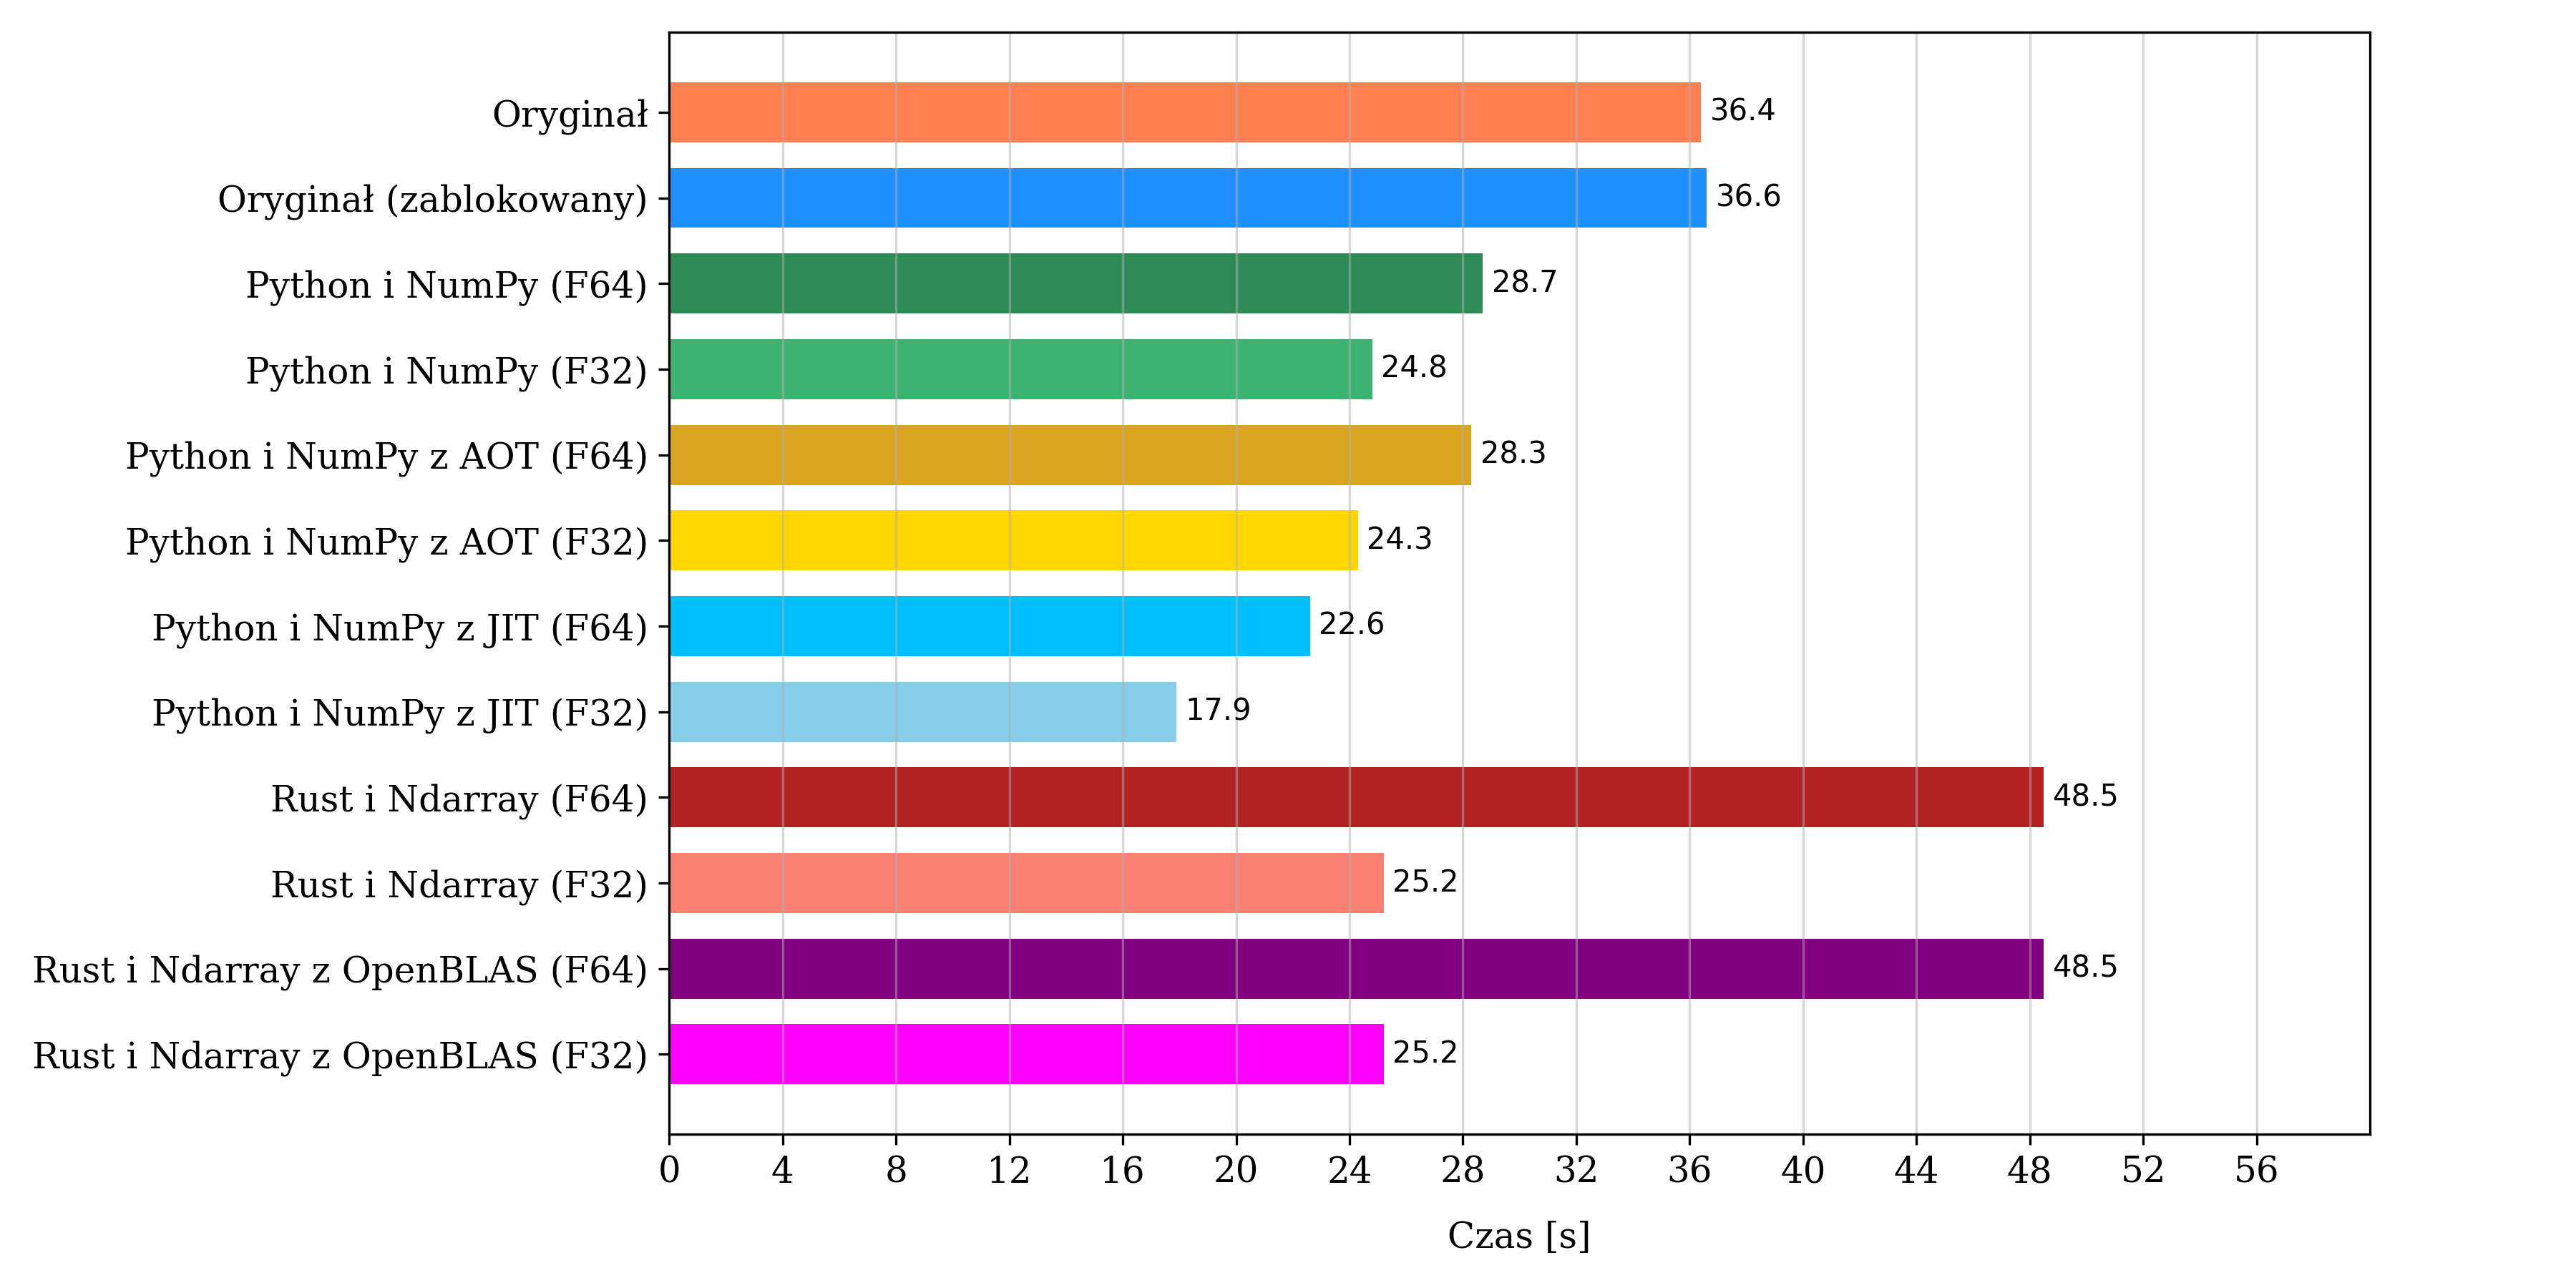
\includegraphics[width=1.0\textwidth]{"resources/rho_1_matrix_comparison.png"}
      \caption{Zestawienie wyników testów wydajności wszystkich implementacji dla macierzy $\rho
      _{1}$.}
      \label{matrix-comparison-rho-1-plot}
    \end{figure}

    Na rysunku \ref{matrix-comparison-rho-1-plot} przedstawione zostało zestawienie
    wyników wydajności dla testów przeprowadzanych przy pomocy macierzy $\rho_{1}$. Najkrótszy
    czas pracy w zestawieniu, $17.9s$, uzyskała implementacja napisana w języku Python z
    użyciem biblioteki NumPy z kompilacją JIT wykonująca obliczenia pojedynczej precyzji.
    Niewiele ustępuje jej wariant pracujący na liczbach podwójnej precyzji z wynikiem
    $22 .6s$.

    \FloatBarrier

    \subsubsection{Macierz \texorpdfstring{$\rho_{2}$ $(4\times4)$}{rho2 4x4}}
    \begin{figure}[ht]
      \centering
      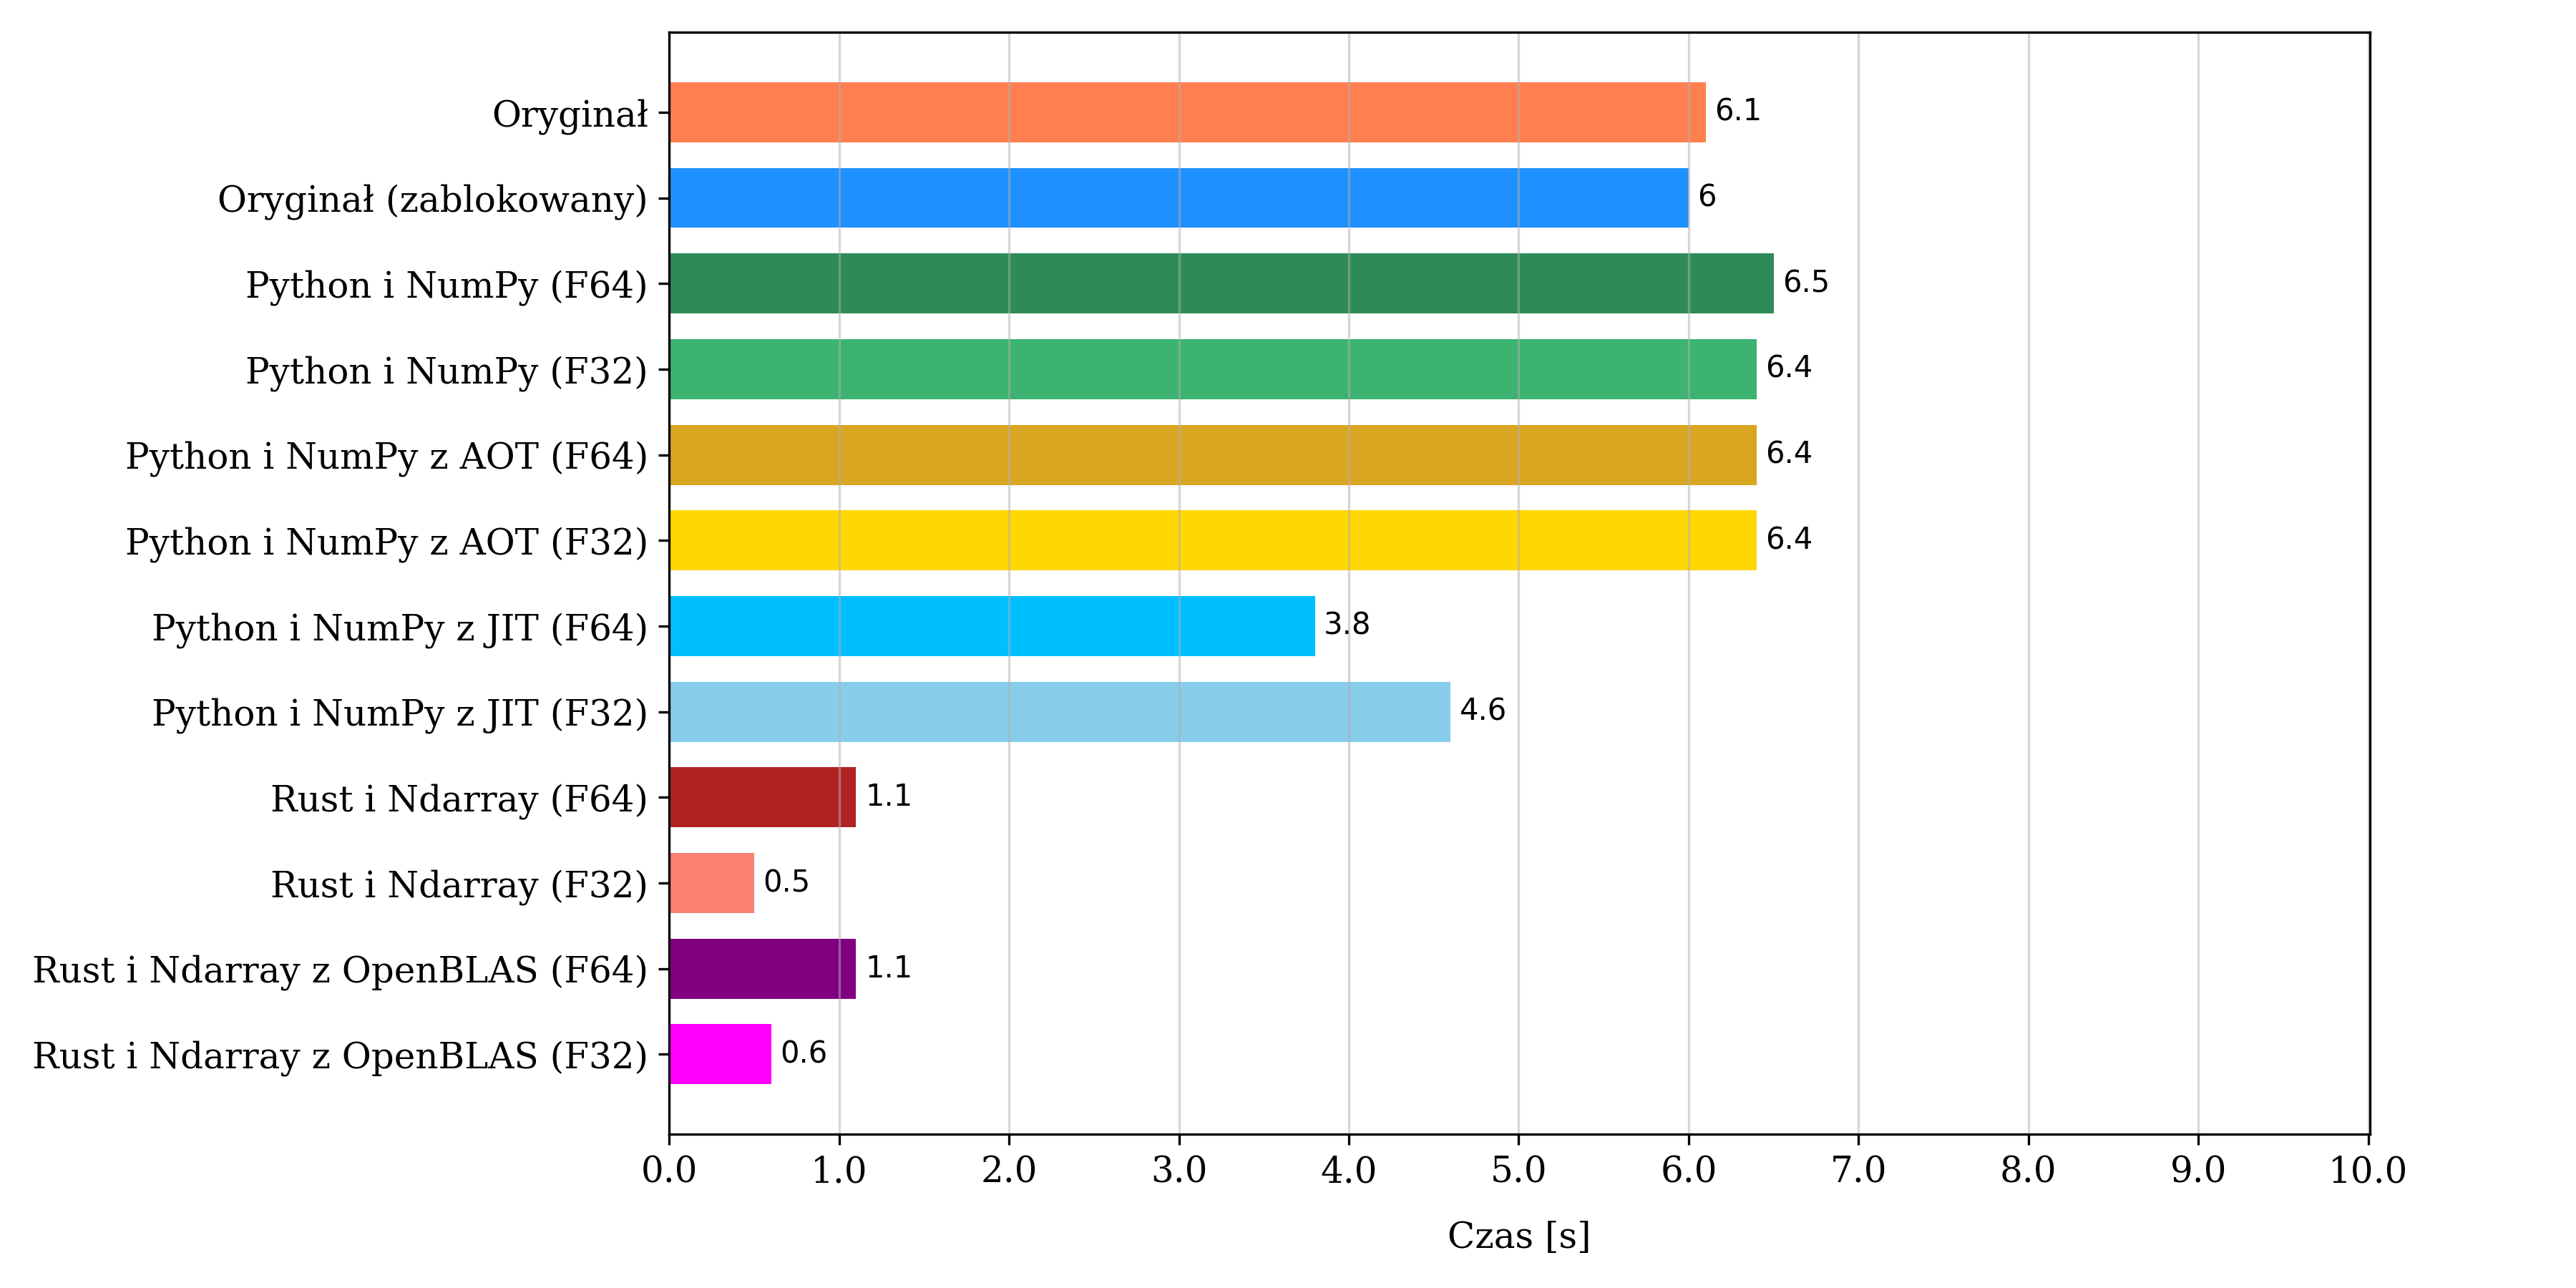
\includegraphics[width=1.0\textwidth]{"resources/rho_2_matrix_comparison.png"}
      \caption{Zestawienie wyników testów wydajności wszystkich implementacji dla macierzy $\rho
      _{2}$.}
      \label{matrix-comparison-rho-2-plot}
    \end{figure}

    Na rysunku \ref{matrix-comparison-rho-2-plot} przedstawione zostało zestawienie
    wyników wydajności dla testów przeprowadzanych przy pomocy macierzy $\rho_{2}$. Najkrótszy
    czas pracy w zestawieniu, $0.5s$, uzyskała implementacja napisana w języku Rust wykonująca
    obliczenia pojedynczej precyzji. Bardzo zbliżony wynik uzyskał wariant korzystający
    z biblioteki OpenBLAS$0.6s$.

    Z pośród implementacji w języku Python najlepiej sprawował się wariant z JIT (F64),
    natomiast jego czas pracy był około $7.6\times$ dłuższy.

    \FloatBarrier

    \subsubsection{Macierz \texorpdfstring{$\rho_{3}$ $(8\times8)$}{rho3 8x8}}
    \begin{figure}[ht]
      \centering
      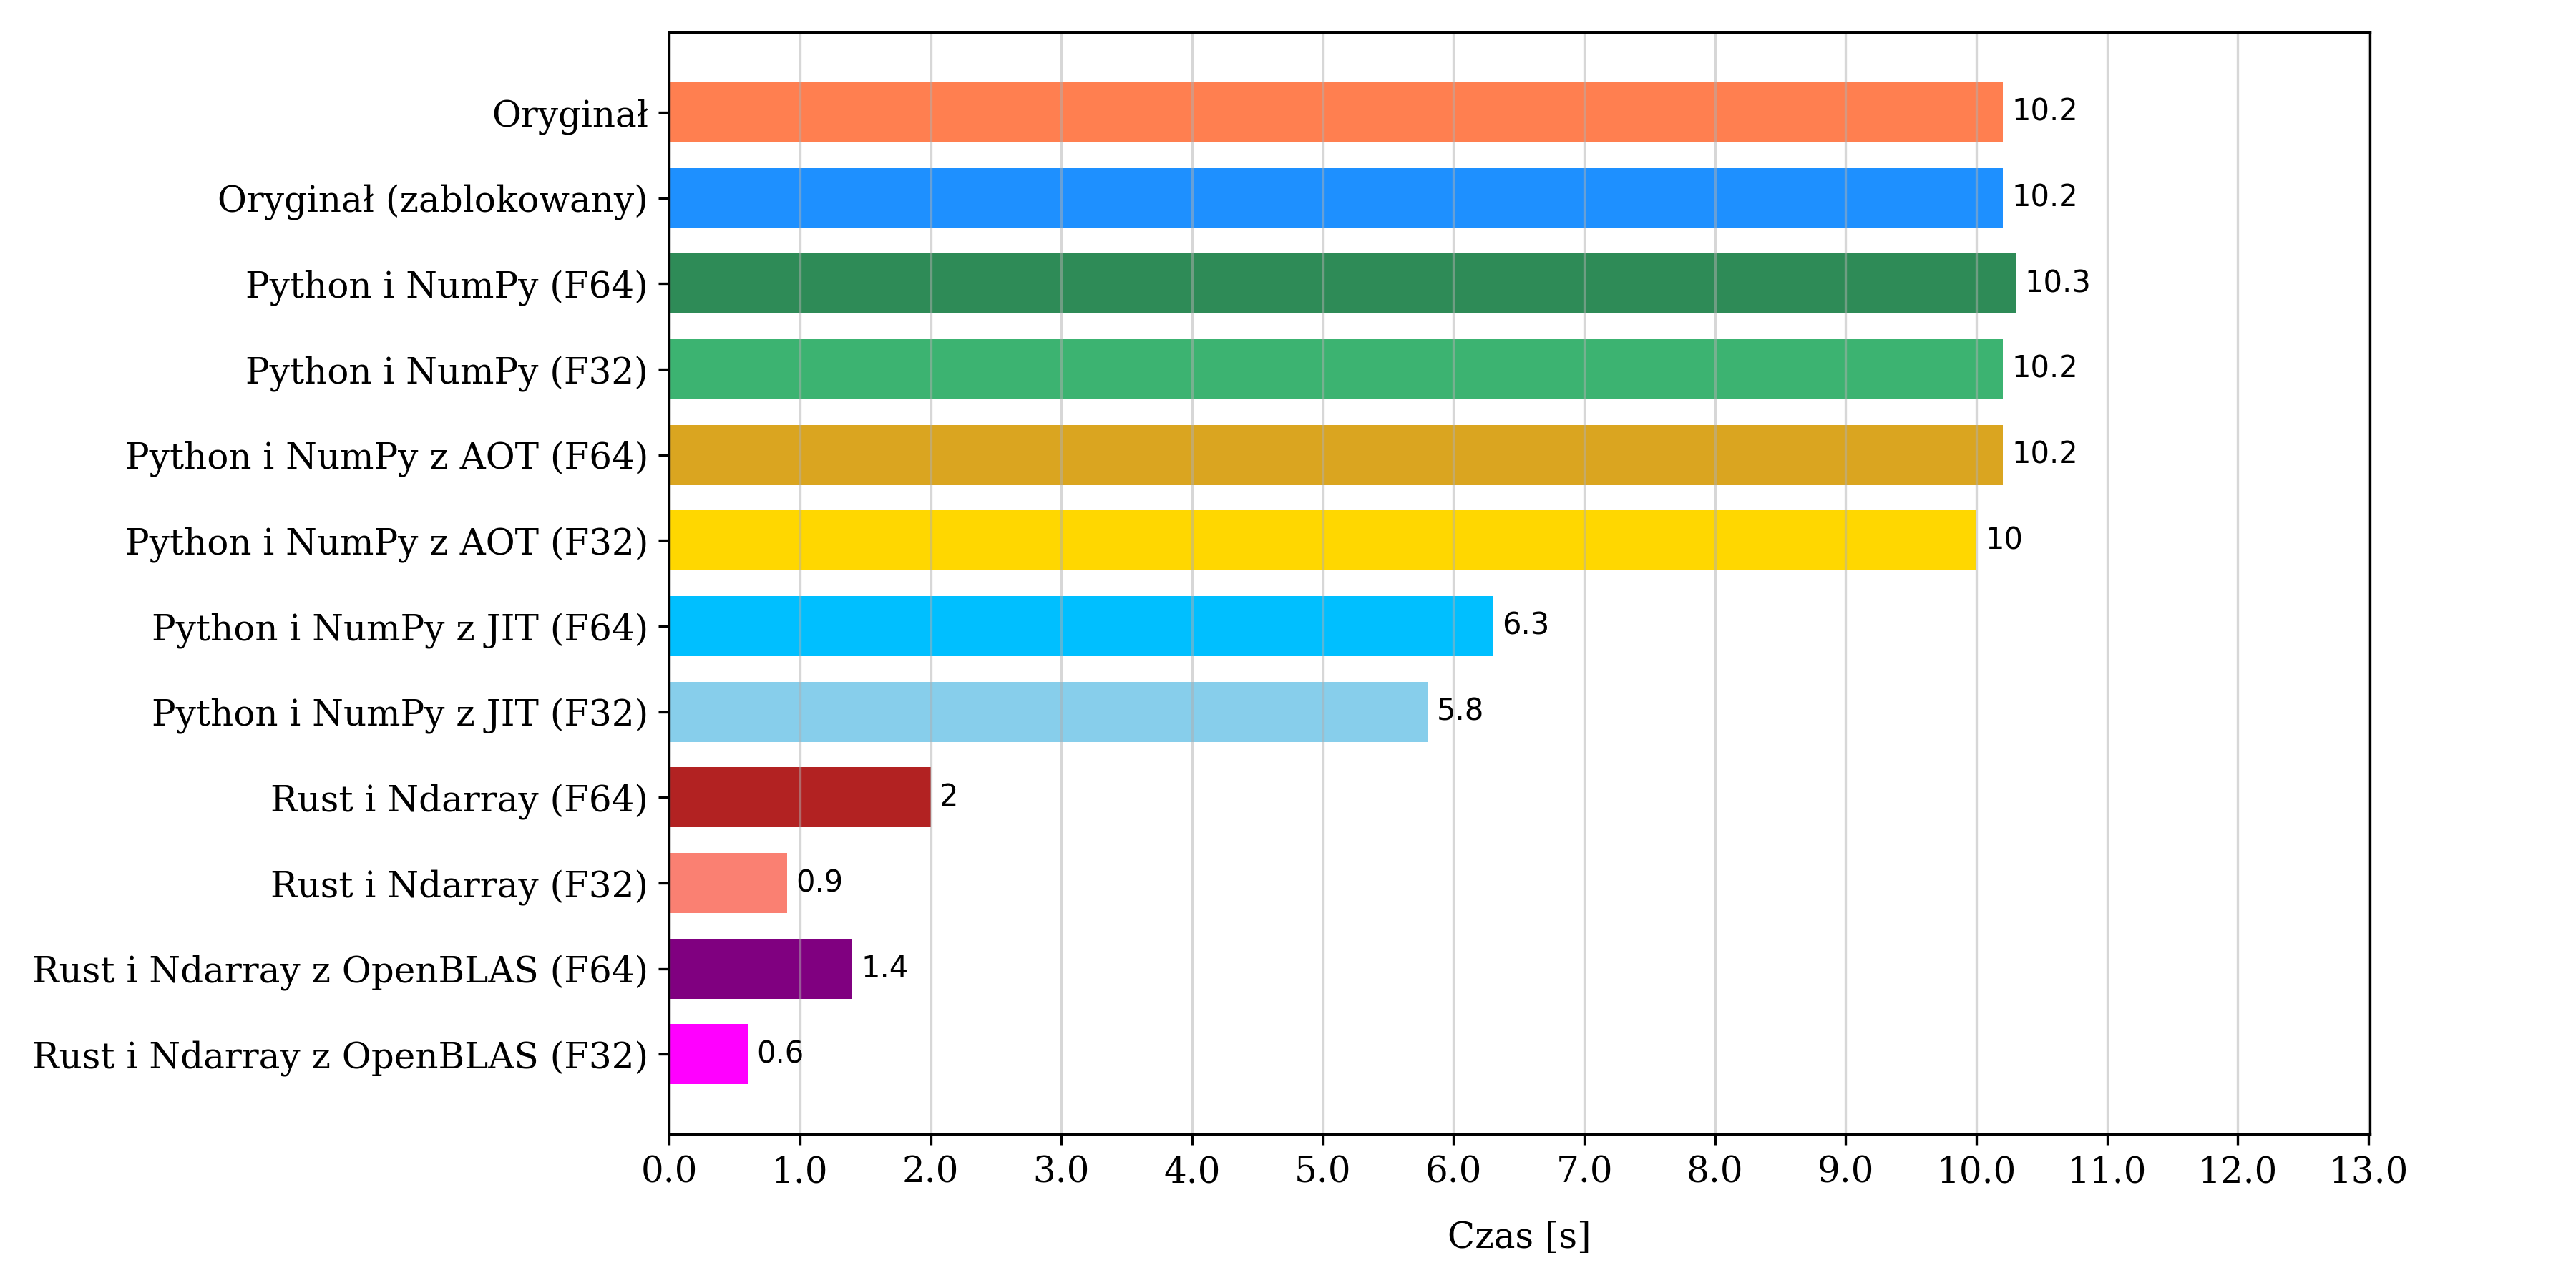
\includegraphics[width=1.0\textwidth]{"resources/rho_3_matrix_comparison.png"}
      \caption{Zestawienie wyników testów wydajności wszystkich implementacji dla macierzy $\rho
      _{3}$.}
      \label{matrix-comparison-rho-3-plot}
    \end{figure}
    Na rysunku \ref{matrix-comparison-rho-3-plot} przedstawione zostało zestawienie wyników
    wydajności dla testów przeprowadzanych przy pomocy macierzy $\rho_{3}$. Najkrótszy
    czas pracy w zestawieniu, $0.6s$, uzyskała implementacja napisana w języku Rust z
    OpenBLAS wykonująca obliczenia pojedynczej precyzji. Bardzo zbliżony wynik uzyskał wariant
    który nie korzystał z OpenBLAS ($0.9s$).

    \FloatBarrier

    \subsubsection{Macierz \texorpdfstring{$\rho_{4}$ $(16\times16)$}{rho4 16x16}}
    \begin{figure}[ht]
      \centering
      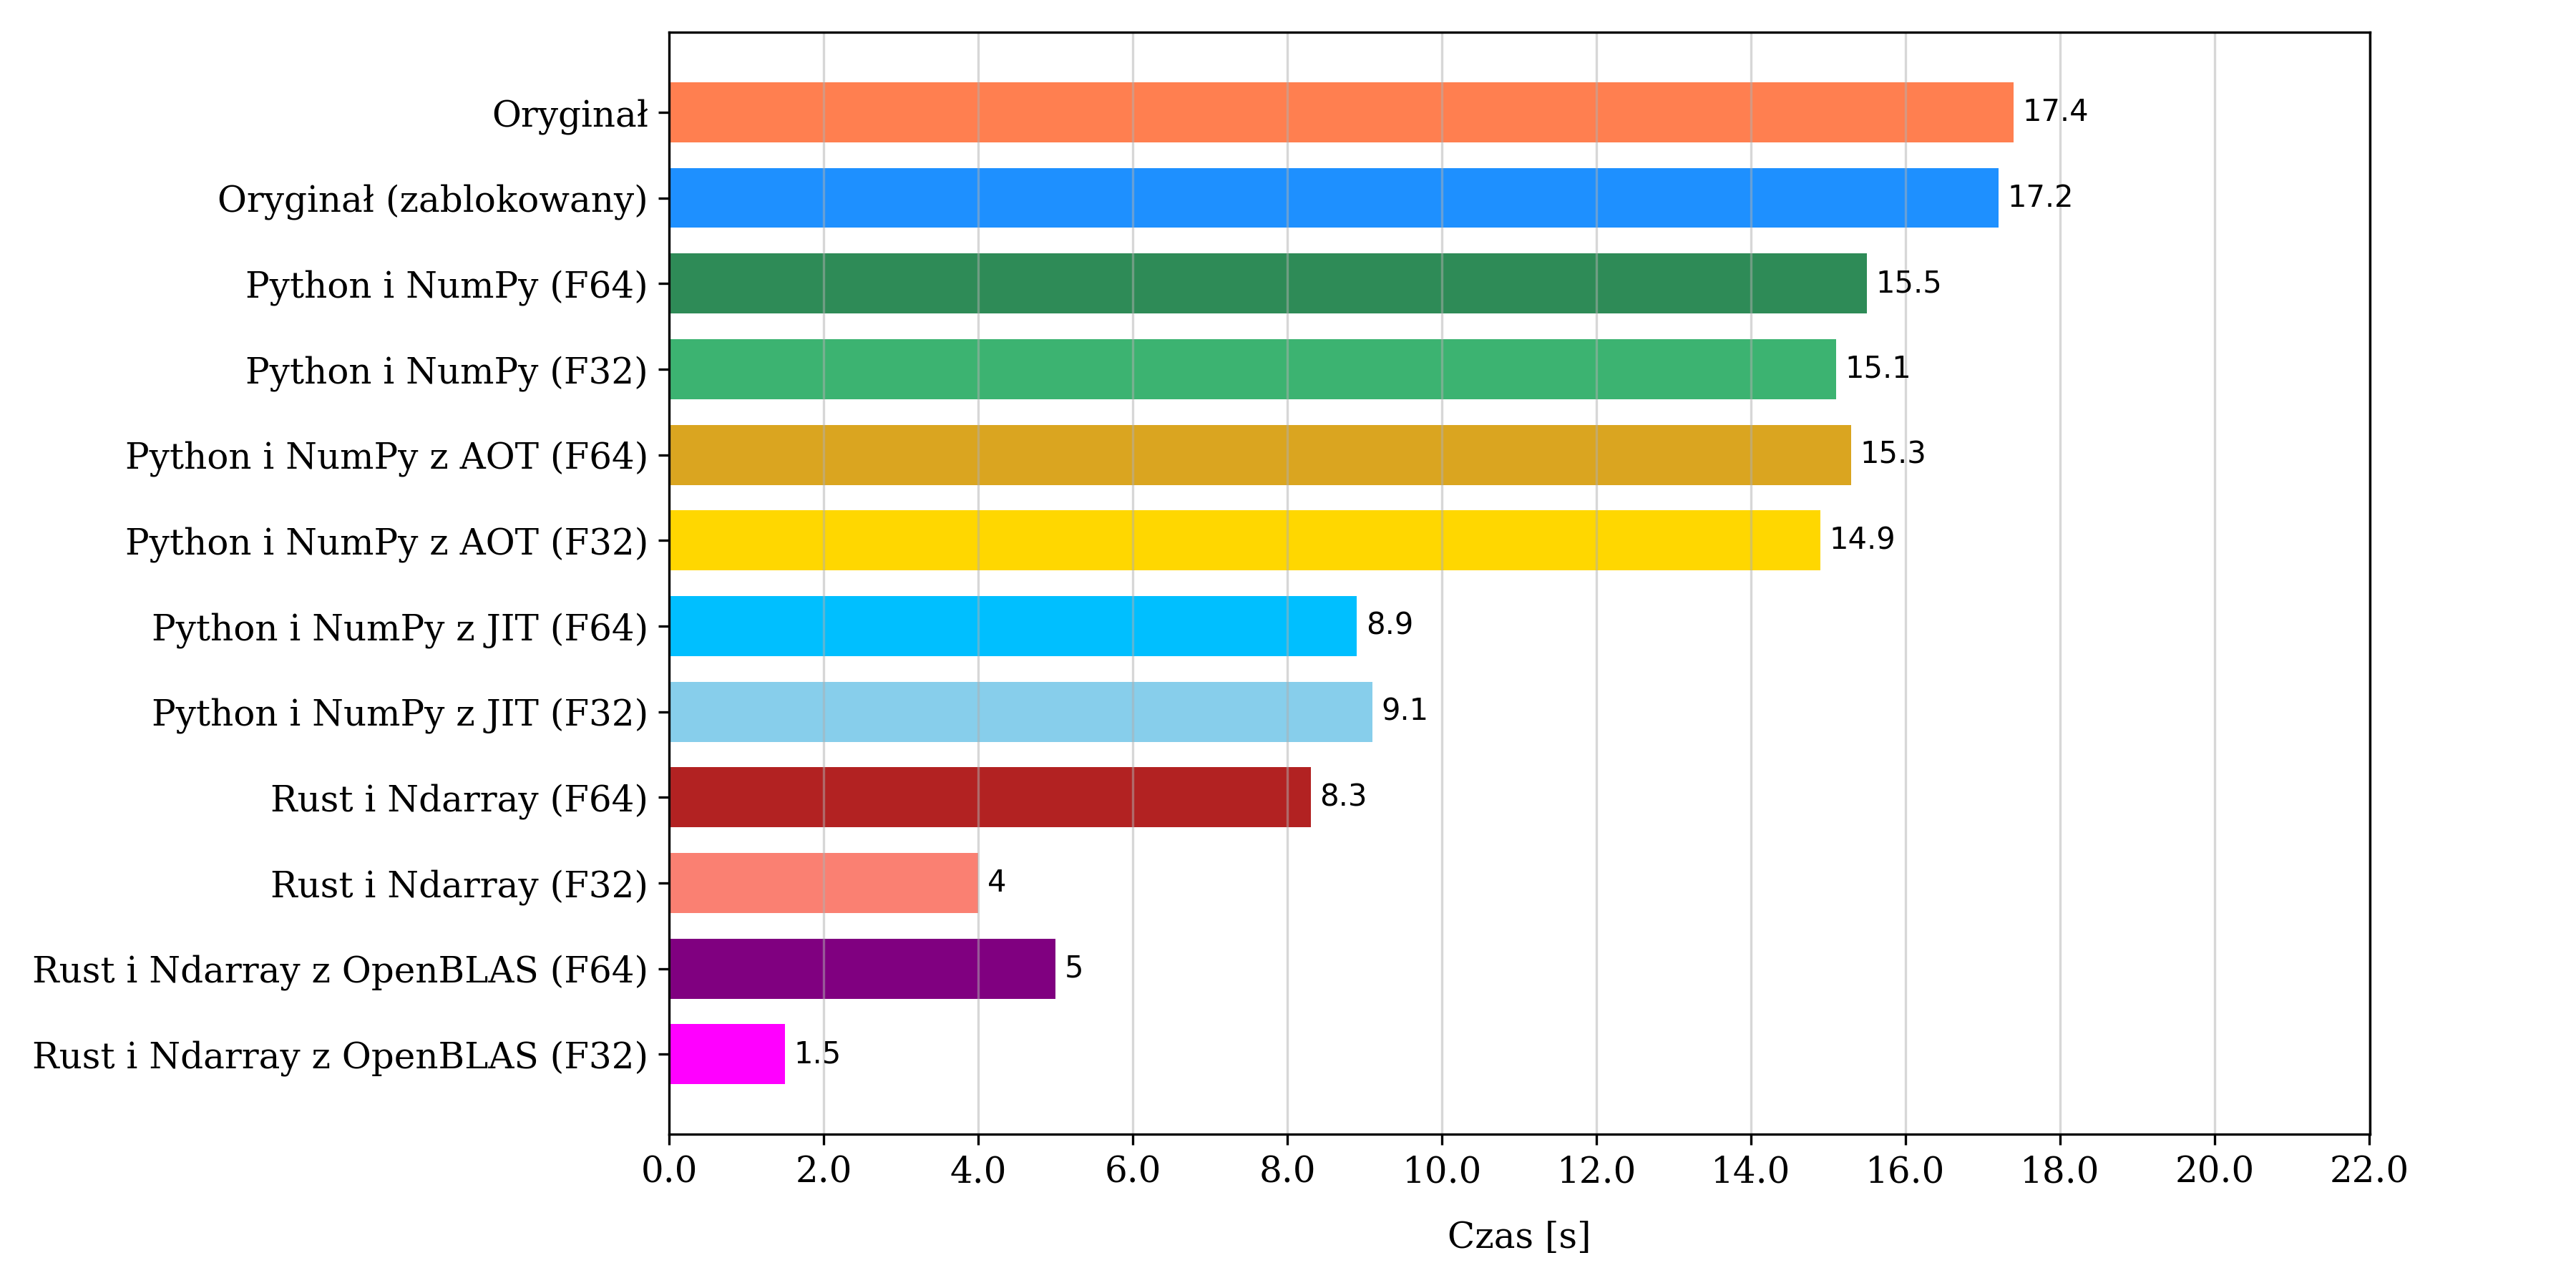
\includegraphics[width=1.0\textwidth]{"resources/rho_4_matrix_comparison.png"}
      \caption{Zestawienie wyników testów wydajności wszystkich implementacji dla macierzy $\rho
      _{4}$.}
      \label{matrix-comparison-rho-4-plot}
    \end{figure}
    Na rysunku \ref{matrix-comparison-rho-4-plot} przedstawione zostało zestawienie
    wyników wydajności dla testów przeprowadzanych przy pomocy macierzy $\rho_{4}$. Najkrótszy
    czas pracy w zestawieniu, $1.5s$, uzyskała implementacja napisana w języku Rust z OpenBLAS
    wykonująca obliczenia pojedynczej precyzji. Bardzo zbliżony wynik uzyskał wariant
    który nie korzystał z OpenBLAS ($4s$).

    \FloatBarrier

    \subsubsection{Macierz \texorpdfstring{$\rho_{5}$ $(32\times32)$}{rho5 32x32}}
    \begin{figure}[ht]
      \centering
      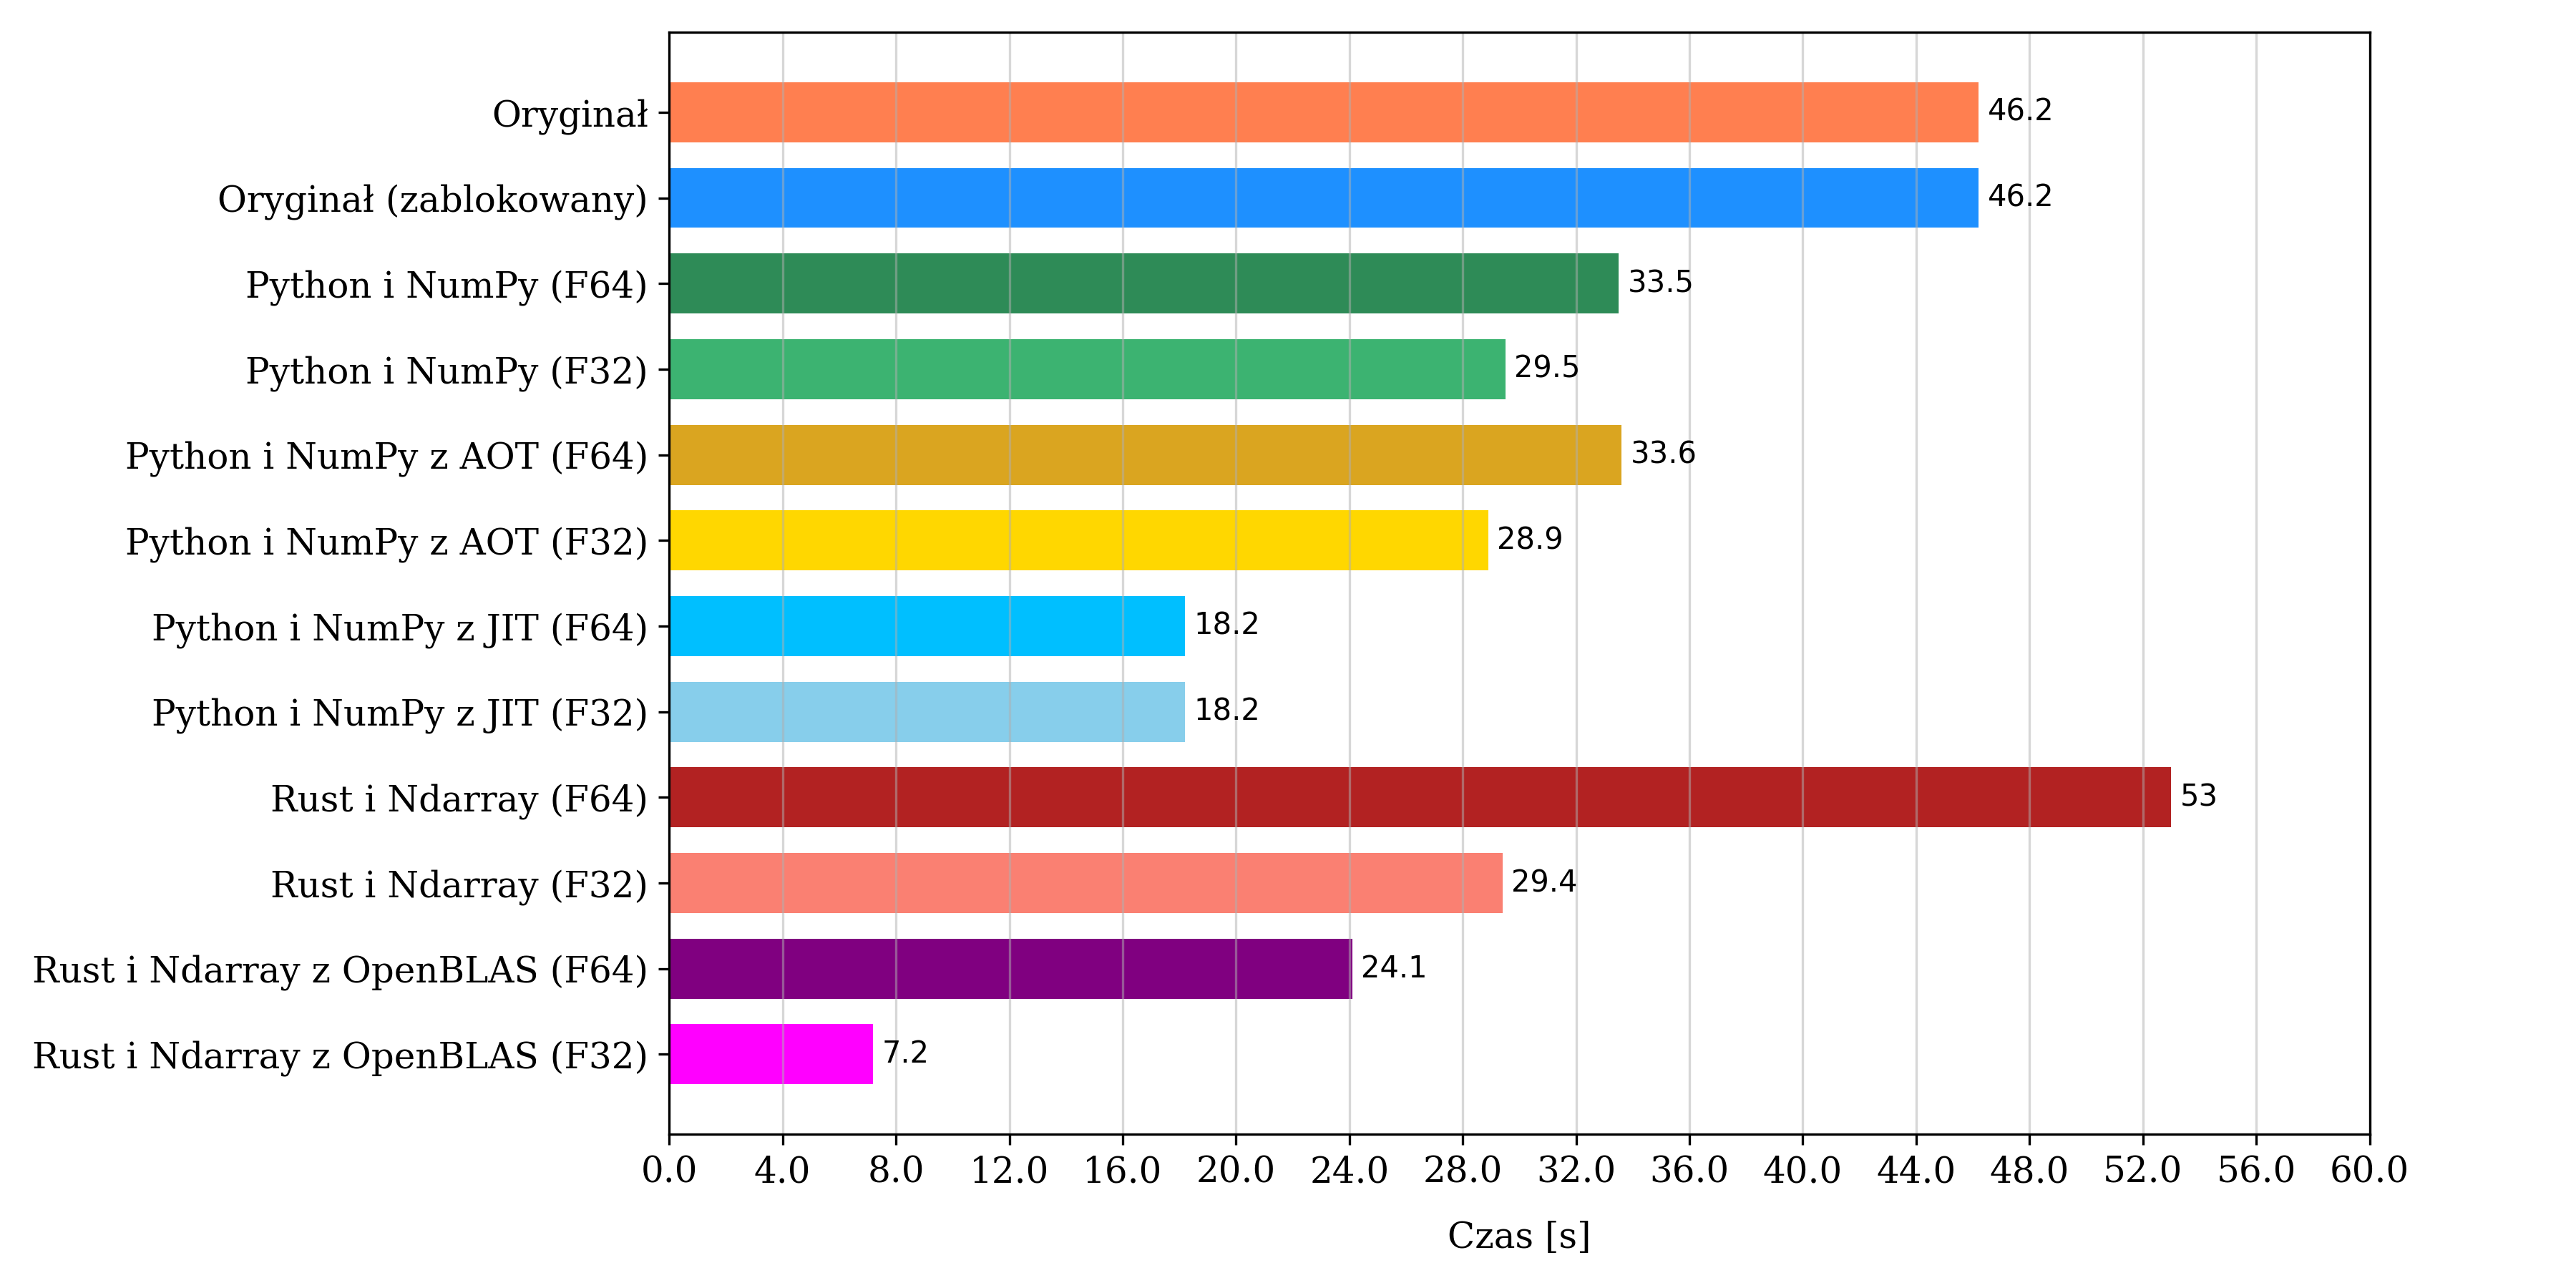
\includegraphics[width=1.0\textwidth]{"resources/rho_5_matrix_comparison.png"}
      \caption{Zestawienie wyników testów wydajności wszystkich implementacji dla macierzy $\rho
      _{5}$.}
      \label{matrix-comparison-rho-5-plot}
    \end{figure}
    Na rysunku \ref{matrix-comparison-rho-5-plot} przedstawione zostało zestawienie wyników
    wydajności dla testów przeprowadzanych przy pomocy macierzy $\rho_{5}$. Najkrótszy
    czas pracy w zestawieniu, $7.2s$, uzyskała implementacja napisana w języku Rust z
    OpenBLAS wykonująca obliczenia pojedynczej precyzji. Następny najniższy wynik wynosił
    $18.2s$ i był osiągany przez wariant w języku Python korzystający z JIT, niezależnie
    od precyzji obliczeń.

    \subsubsection{Macierz \texorpdfstring{$\rho_{6}$ $(64\times64)$}{rho6 64x64}}
    \begin{figure}[ht]
      \centering
      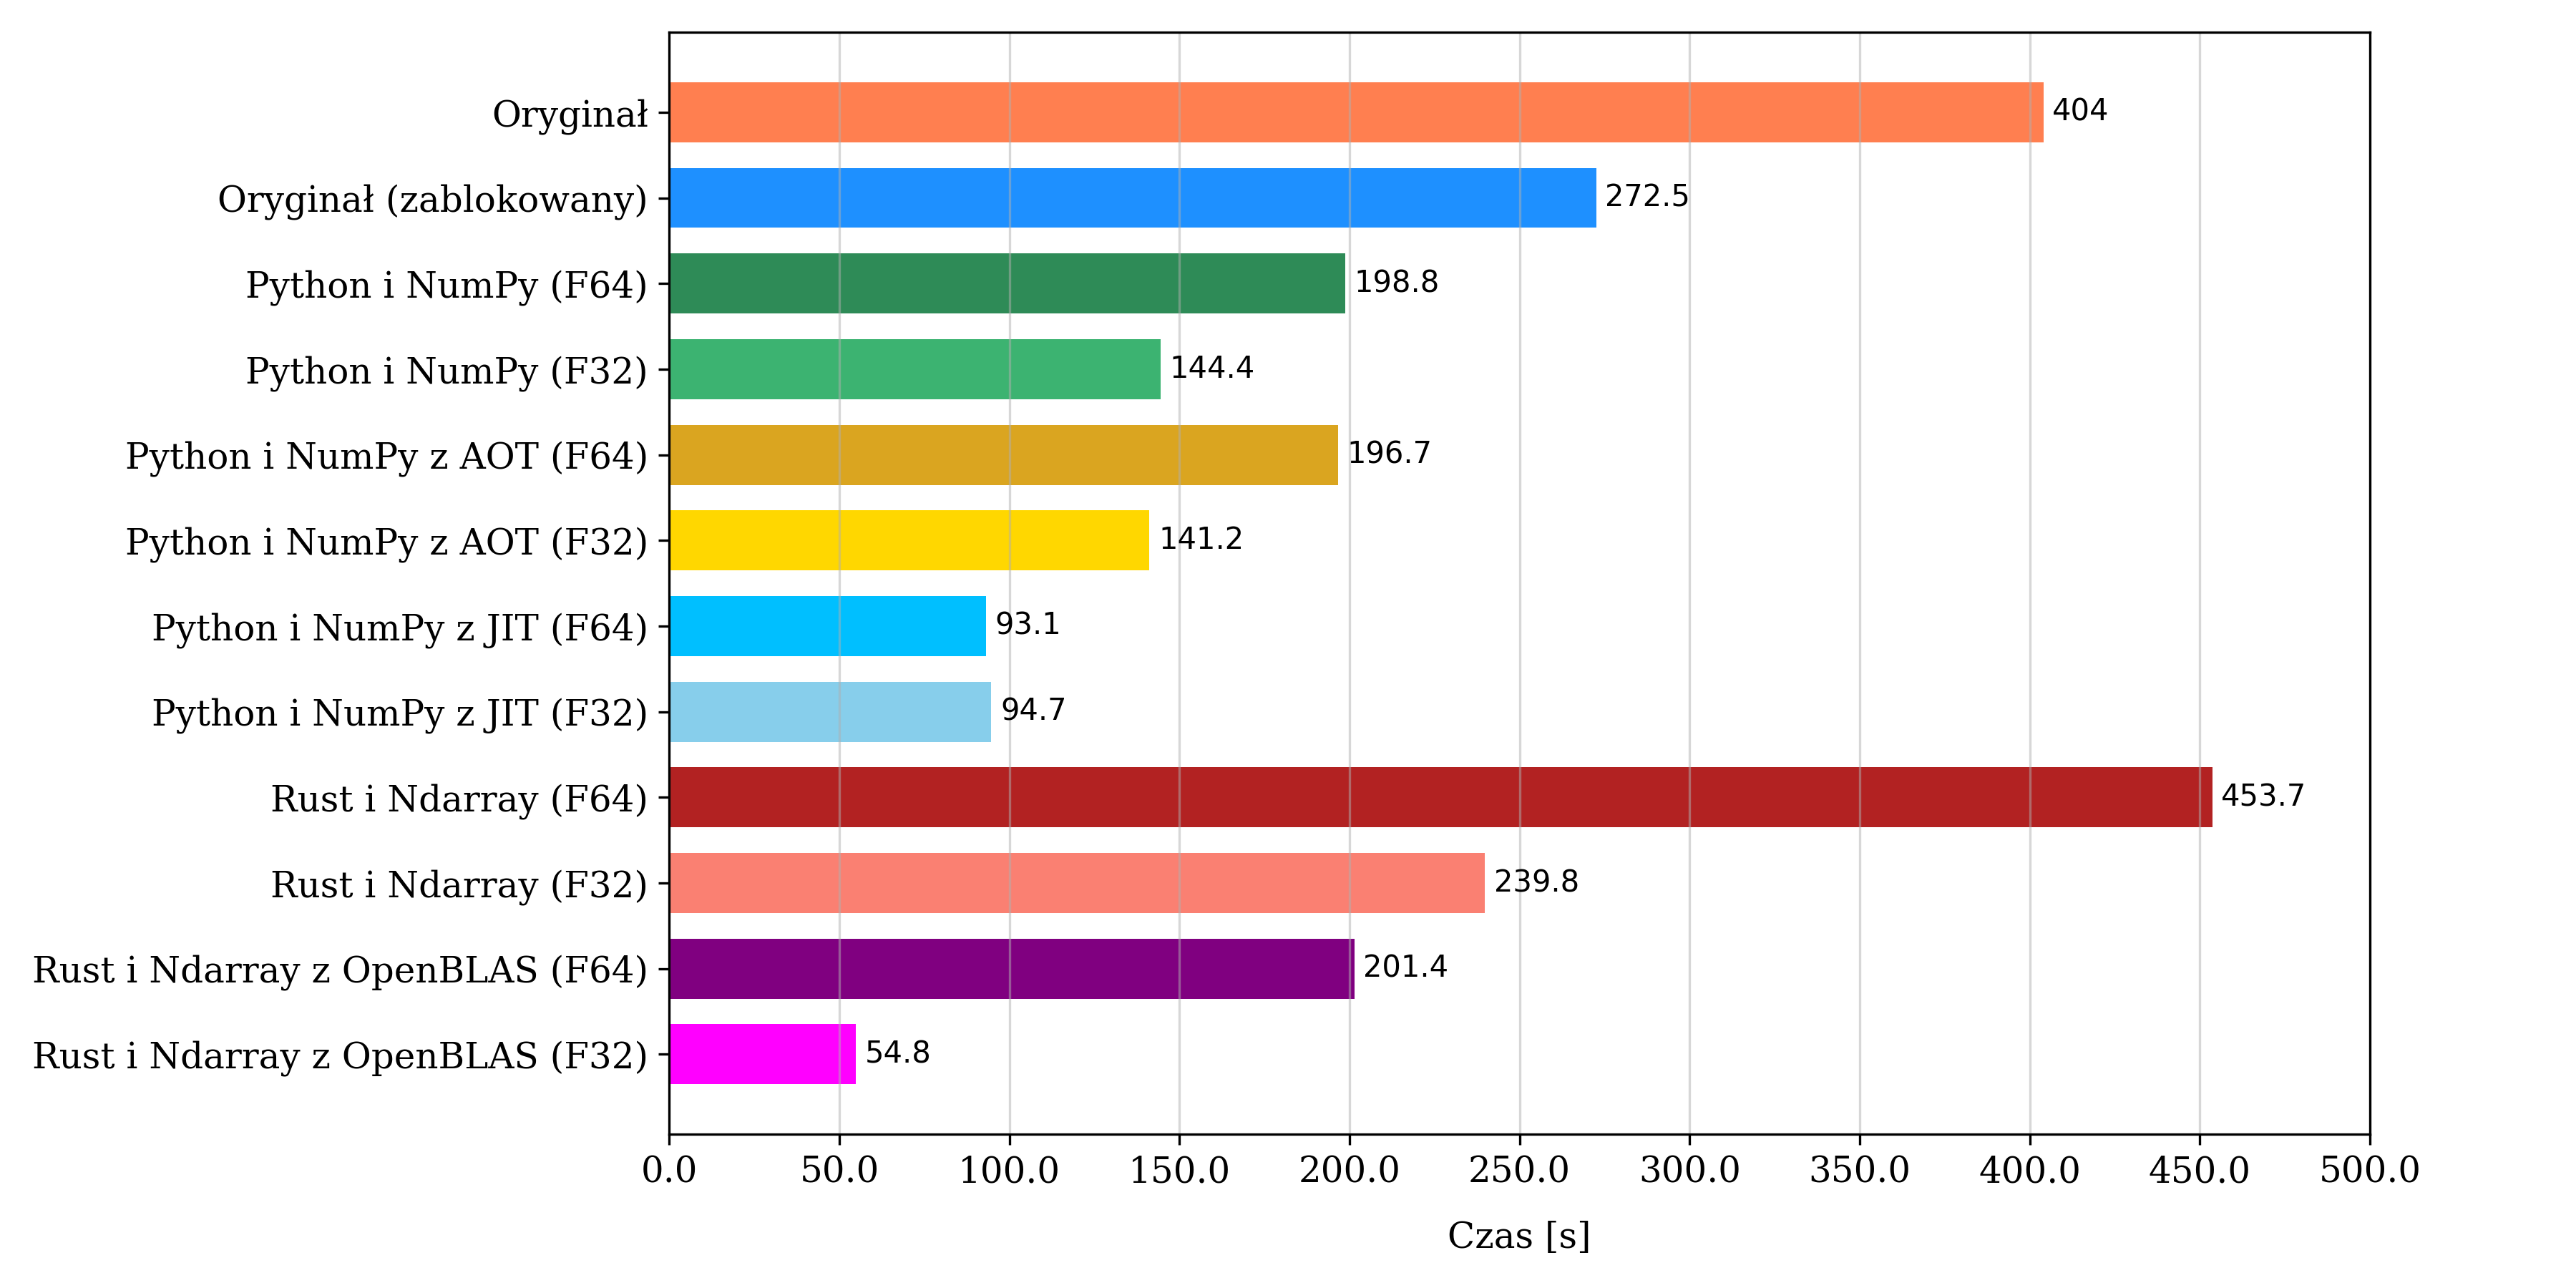
\includegraphics[width=1.0\textwidth]{"resources/rho_6_matrix_comparison.png"}
      \caption{Zestawienie wyników testów wydajności wszystkich implementacji dla macierzy $\rho
      _{6}$.}
      \label{matrix-comparison-rho-6-plot}
    \end{figure}
    Na rysunku \ref{matrix-comparison-rho-6-plot} przedstawione zostało zestawienie
    wyników wydajności dla testów przeprowadzanych przy pomocy macierzy $\rho_{6}$. Najkrótszy
    czas pracy w zestawieniu, $54.8s$, uzyskała implementacja napisana w języku Rust z OpenBLAS
    wykonująca obliczenia pojedynczej precyzji. Następny najniższy wynik wynosił $93.1s$
    i był osiągany przez wariant w języku Python korzystający z JIT przy obliczeniach
    podwójnej precyzji. Kod wykonujący obliczenia pojedynczej precyzji wypadł nieznacznie
    gorzej.

    \FloatBarrier

    \subsection{Pomiary dla wielu zadań}


    \section{Dyskusja}


    Praca ta miała na celu eksplorację dostępnych metod maksymalizacji wydajności
    algorytmu QGA. Udało mi się w jej ramach zbadać skuteczność wykorzystania dziesięciu
    wariantów programu, w tym dwóch implementacji w różnych językach programowania. Algorytm
    QGA został z powodzeniem wielokrotnie zaimplementowany, a wszystkie stworzone
    implementacje pozwalały uzyskać oczekiwane wyniki liczbowe.

    Przeprowadziłem również liczne testy wydajności dla różnych danych wejściowych dla
    wszystkich wariantów programu, co pozwoliło mi ustalić które metody okazały się najbardziej
    skuteczne. W przypadku dwóch wariantów programu, udało się się uzyskać znaczącą poprawę
    wydajności. Są nimi:
    \begin{enumerate}
      \item Python i NumPy z JIT

      \item Rust i Ndarray z OpenBLAS
    \end{enumerate}
    Z zastrzeżeniem, że w przypadku wariantu 1. dotyczy to zarówno obliczeń podwójnej
    jak i pojedynczej precyzji, natomiast w przypadku 2. znacząca poprawa występowała dla
    obliczeń pojedynczej precyzji.

    Ponadto, stworzony przeze mnie kod został zamieszczony w trzech repozytoriach:
    \begin{enumerate}
      \item cssfinder\cite{CSSFinder_New},

      \item cssfinder\_backend\_numpy\cite{CSSFinder_New_Numpy},

      \item cssfinder\_backend\_rust\cite{CSSFinder_New_Rust},
    \end{enumerate}

    Dla każdego z tych repozytorium istnieje odpowiadający pakiet menadżera pakietów pip
    zamieszczony na serwerze PyPI. Pozwala to w bardzo prosty sposób rozpocząć korzystanie
    z programu poprzez instalację następujących pakietów:
    \begin{enumerate}
      \item cssfinder\cite{CSSFinder_New_PyPI},

      \item cssfinder\_backend\_numpy\cite{CSSFinder_New_Numpy_PyPI},

      \item cssfinder\_backend\_rust\cite{CSSFinder_New_Rust_PyPI},
    \end{enumerate}

    Pakiety są kompatybilne z systemami Linux, MacOS i Windows. Wymagają interpretera języka
    Python w wersji 3.8 lub nowszej.
  \end{sloppypar}
  \newpage
  \begin{sloppypar}
    \medskip


    \printbibliography
    [heading=bibintoc, title={Odwołania}]
  \end{sloppypar}
\end{document}